
\subsection{Comparison of Decompositions}
Time for some plots!
Running example: $g(x_1, x_2) = x_1 + 2 x_2 + x_1 x_2$, with polynomial coefficients: $a_0 = 0$, $a_1 = 1$, $a_2 = 2$, $a_{11} = 0$, $a_{22} = 0$, $a_{12} = 1$ and $\rho = 0$.
Under independent inputs, the fANOVA components are given by:
\begin{align*}
y_{\emptyset} &= 0, \\
y_1(x_1) &= x_1\\
y_2(x_2) &= 2x_2\\
y_{12}(x_1, x_2) &= x_1x_2,
\end{align*}
visualized in \autoref{fig:main_effects_ex1} and \autoref{fig:contour_ex1}. One could vary the magnitude of the coefficients and obtain steeper, flatter, twisted (?) slopes for the main effects and also a steeper of flatter or twisted surface for the interaction term.
% Input: MVN, centred, independent
\begin{figure}[htpb]
    \centering
    \begin{minipage}[t]{0.49\textwidth}
        \centering
        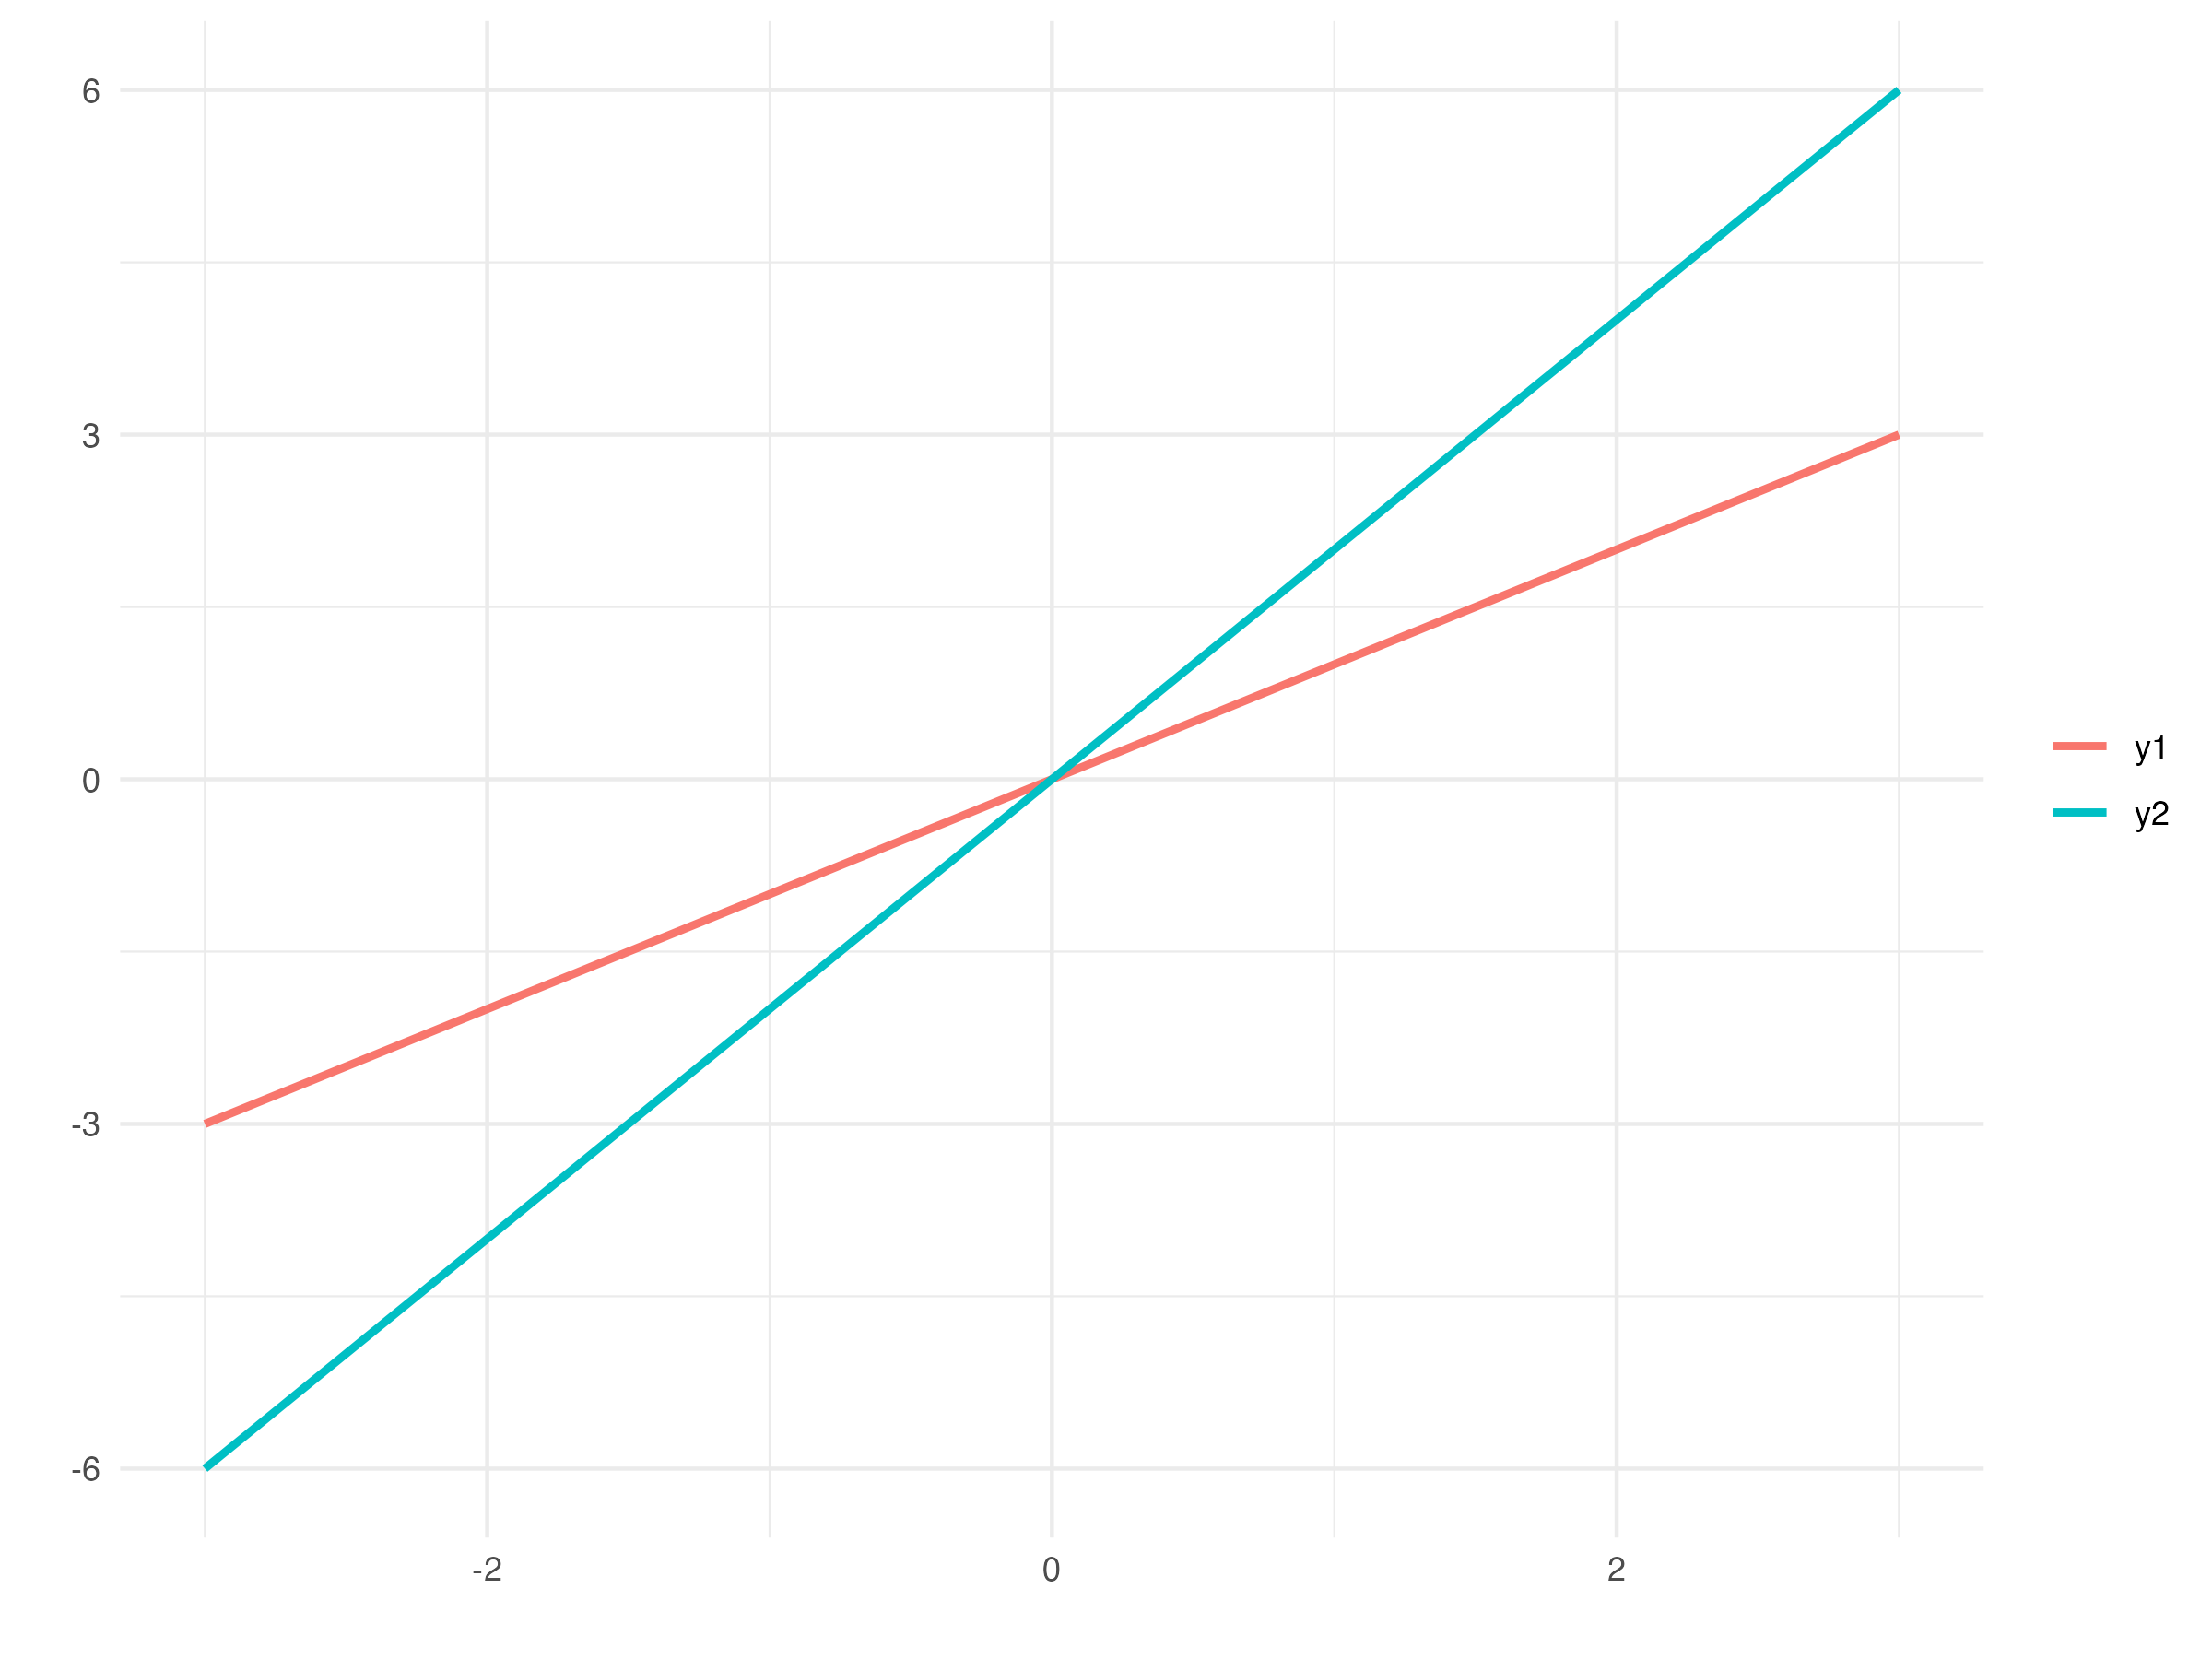
\includegraphics[width=\textwidth]{images/p_main_effect_ex1.png}
        \caption{Main terms as calculated via classical fANOVA for $g(x) = x_1 + 2 x_2 + x_1 x_2$.}
        \label{fig:main_effects_ex1}
    \end{minipage}%
    \hfill
    \begin{minipage}[t]{0.49\textwidth}
        \centering
        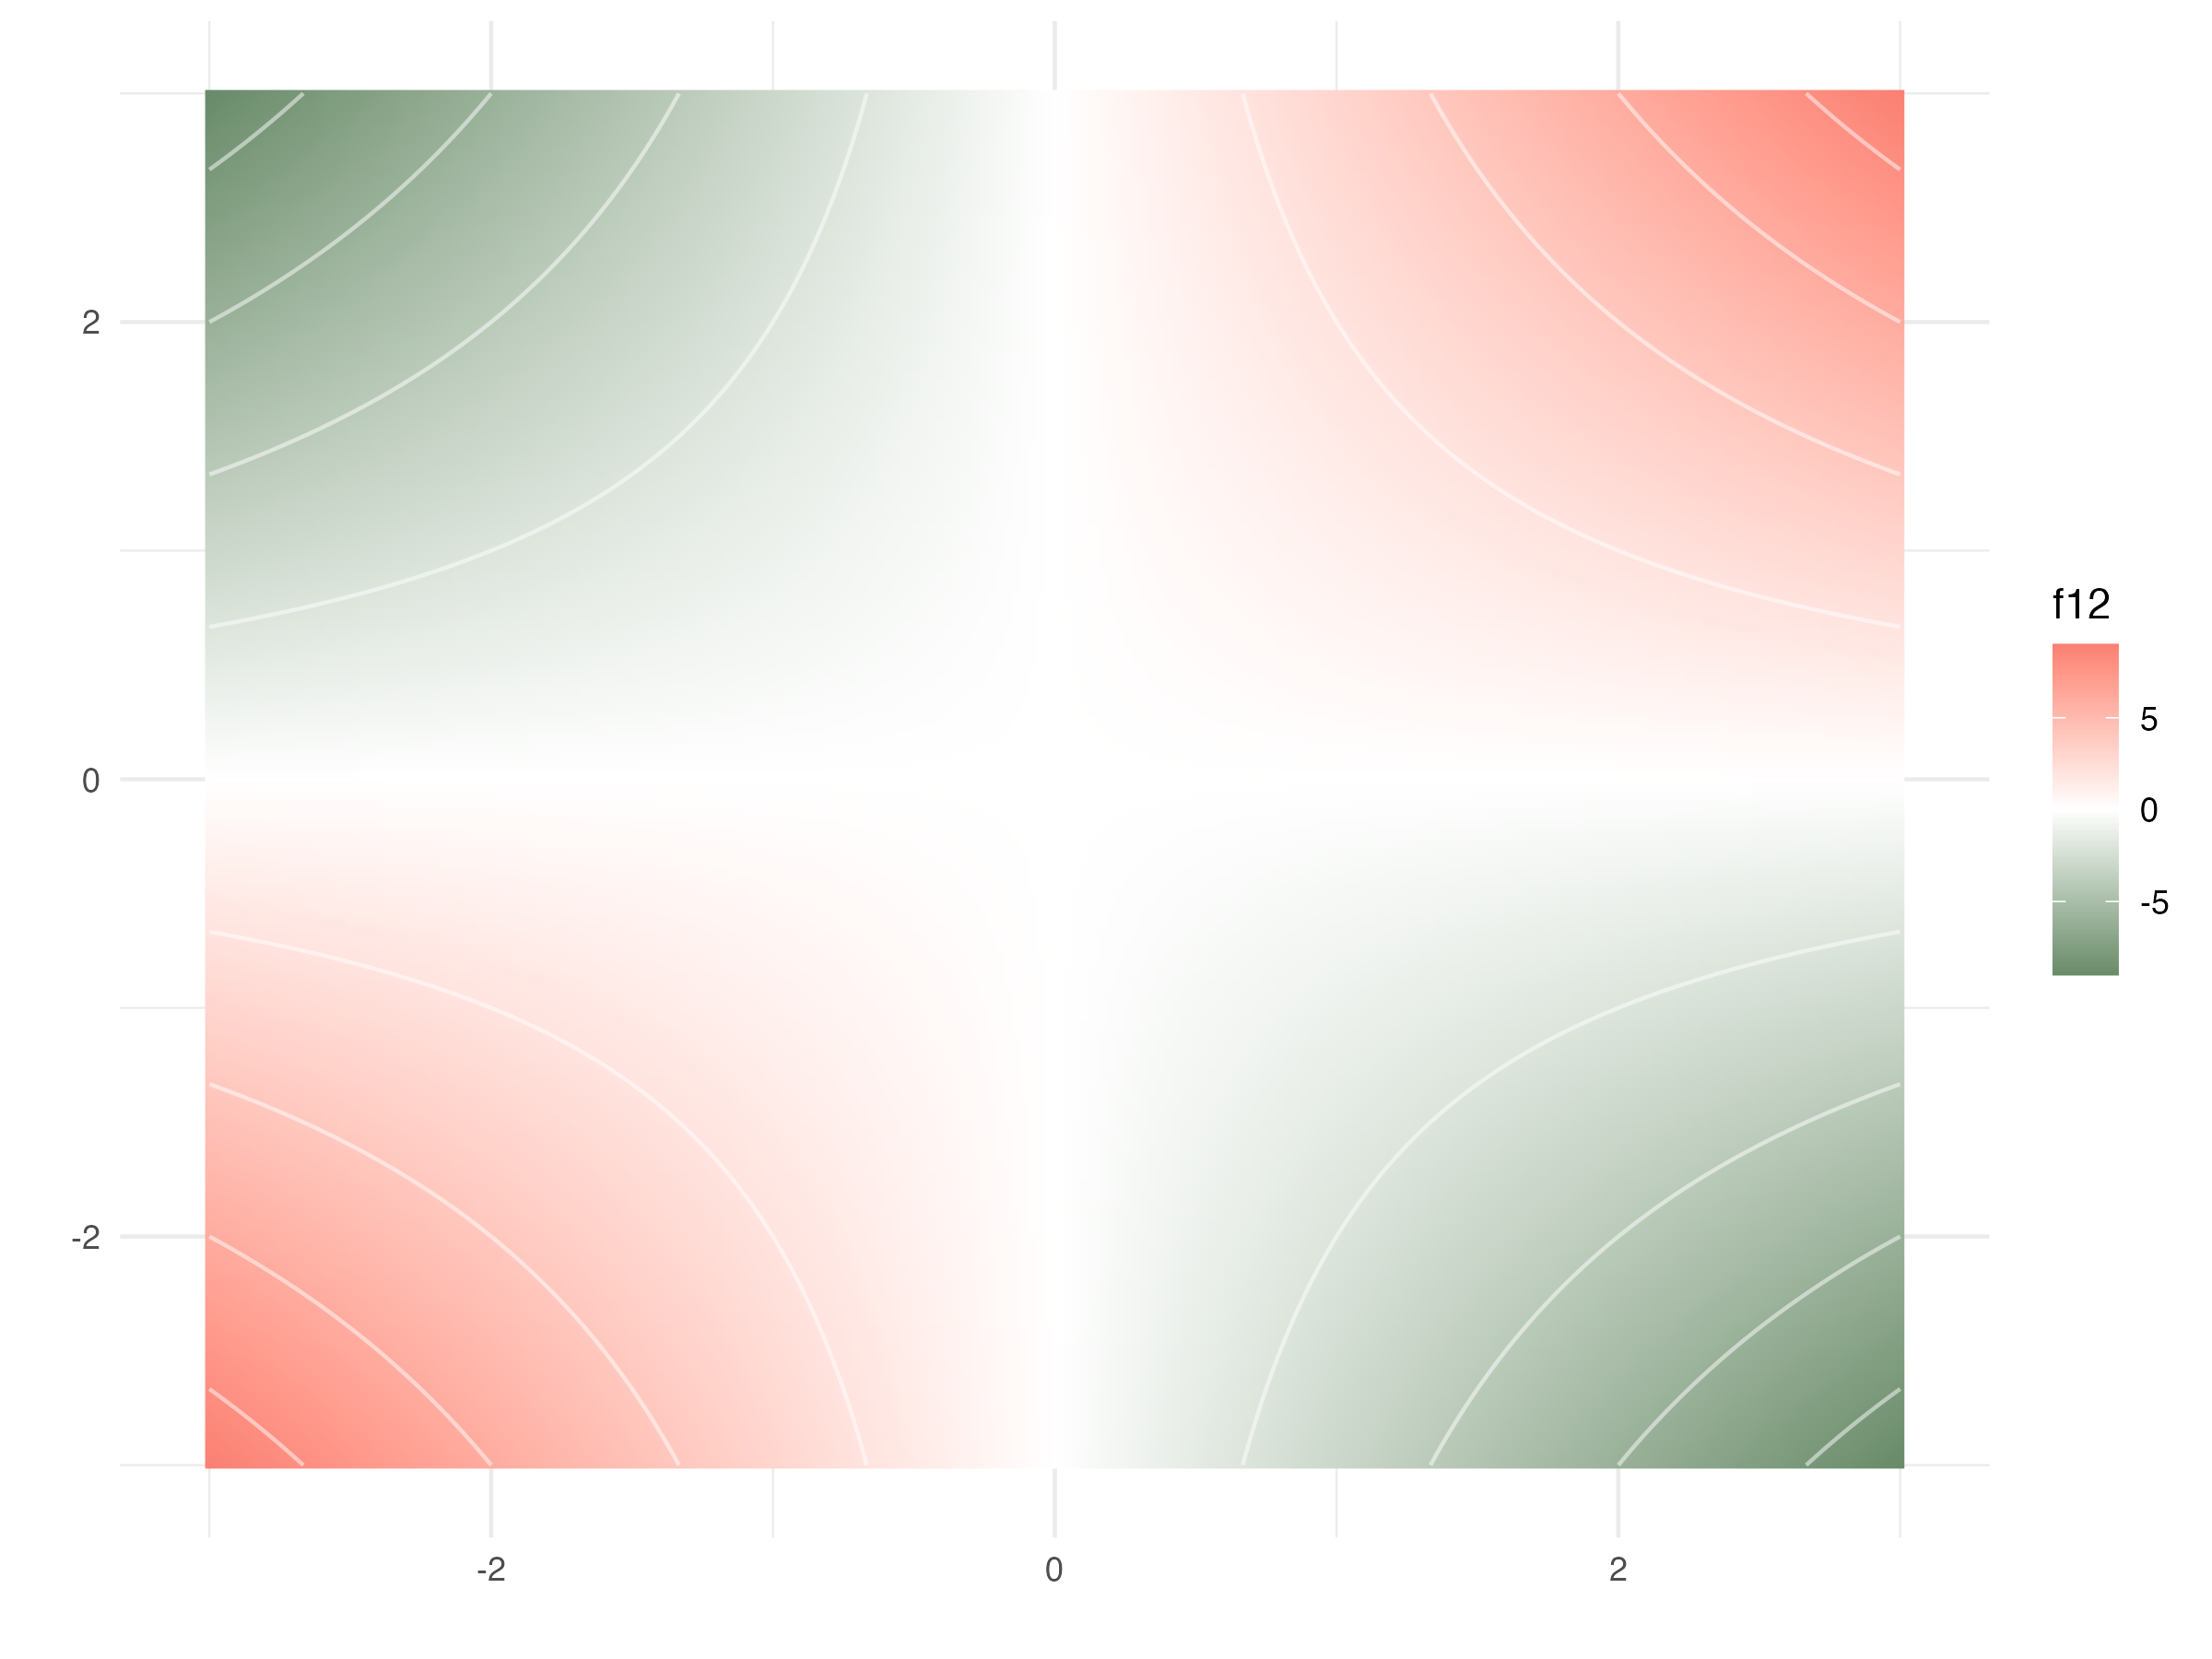
\includegraphics[width=\textwidth]{images/p_contour_ex1.png}
        \caption{Contour plot of $g(x) = x_1 + 2 x_2 + x_1 x_2$.}
        \label{fig:contour_ex1}
    \end{minipage}
\end{figure}

Running example: $g(x_1, x_2) = x_1 + 2 x_2 + x_1 x_2$, with polynomial coefficients: $a_0 = 0$, $a_1 = 1$, $a_2 = 2$, $a_{11} = 0$, $a_{22} = 0$, $a_{12} = 1$ and $\rho = 0.5$.
In attempt to compute the fANOVA terms under dependent inputs, we calculated the following effects, which are in reality the components of the Hoeffding decomposition:

\begin{align*}
\tilde{y}_0 &= a + 0.5 \\[3pt]
\tilde{y}_1(x_1) &= x_1 + 0.5\,(2x_1 + x_1^2 - 1)
= x_1 + x_1 + 0.5x_1^2 - 0.5
= 2x_1 + 0.5x_1^2 - 0.5 \\[3pt]
\tilde{y}_2(x_2) &= 2x_2 + 0.5\,(x_2 + x_2^2 - 1)
= 2x_2 + 0.5x_2 + 0.5x_2^2 - 0.5
= 2.5x_2 + 0.5x_2^2 - 0.5 \\[3pt]
\tilde{y}_{12}(x_1,x_2) &= x_1x_2 - 2(0.5)x_1 - (0.5)x_2 - (0.5)x_1^2 - (0.5)x_2^2 + 0.5 \\[3pt]
&= x_1x_2 - x_1 - 0.5x_2 - 0.5x_1^2 - 0.5x_2^2 + 0.5,
\end{align*}
which are visualized in \autoref{fig:hoeffding_rho05} and \autoref{fig:hoeffding_contour_rho05}.
\begin{figure}[htpb]
    \centering
    \begin{minipage}[t]{0.49\textwidth}
        \centering
        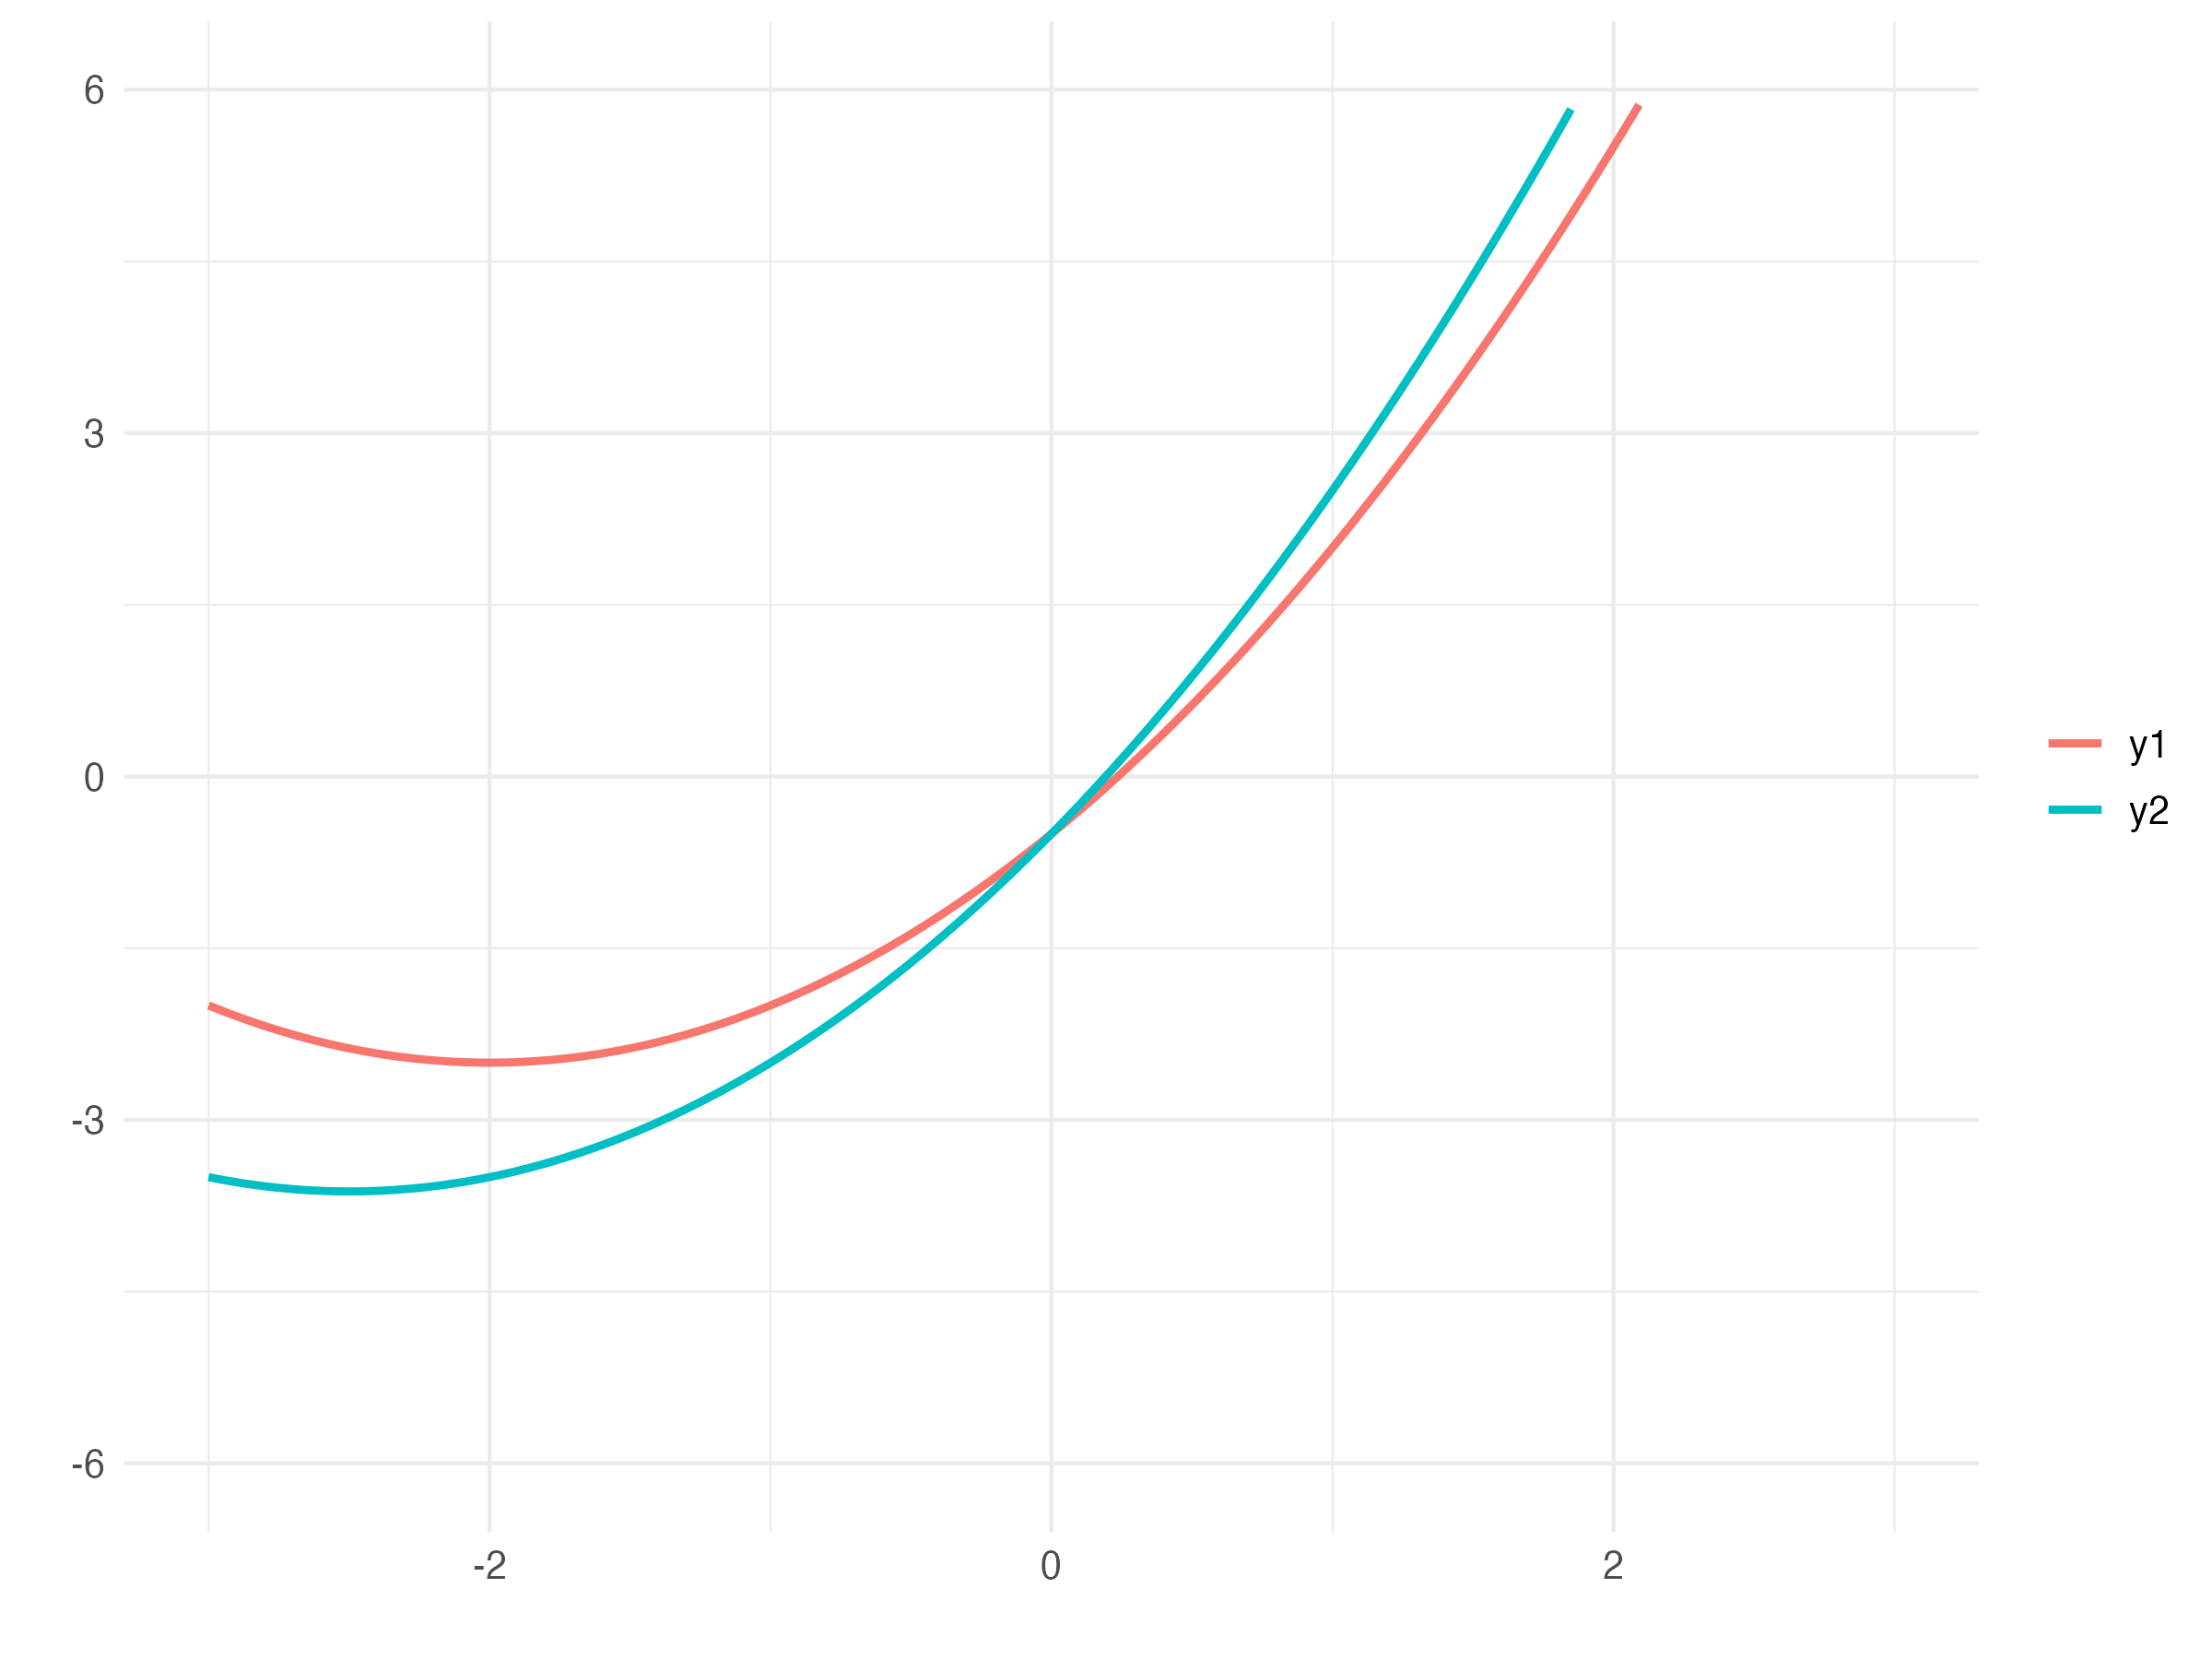
\includegraphics[width=\textwidth]{images/hoeffding_rho05.png}
        \caption{Hoeffding decomposition of $g(x) = x_1 + 2 x_2 + x_1 x_2$ with $\rho = 0.5$.}
        \label{fig:hoeffding_rho05}
    \end{minipage}%
    \hfill
    \begin{minipage}[t]{0.49\textwidth}
        \centering
        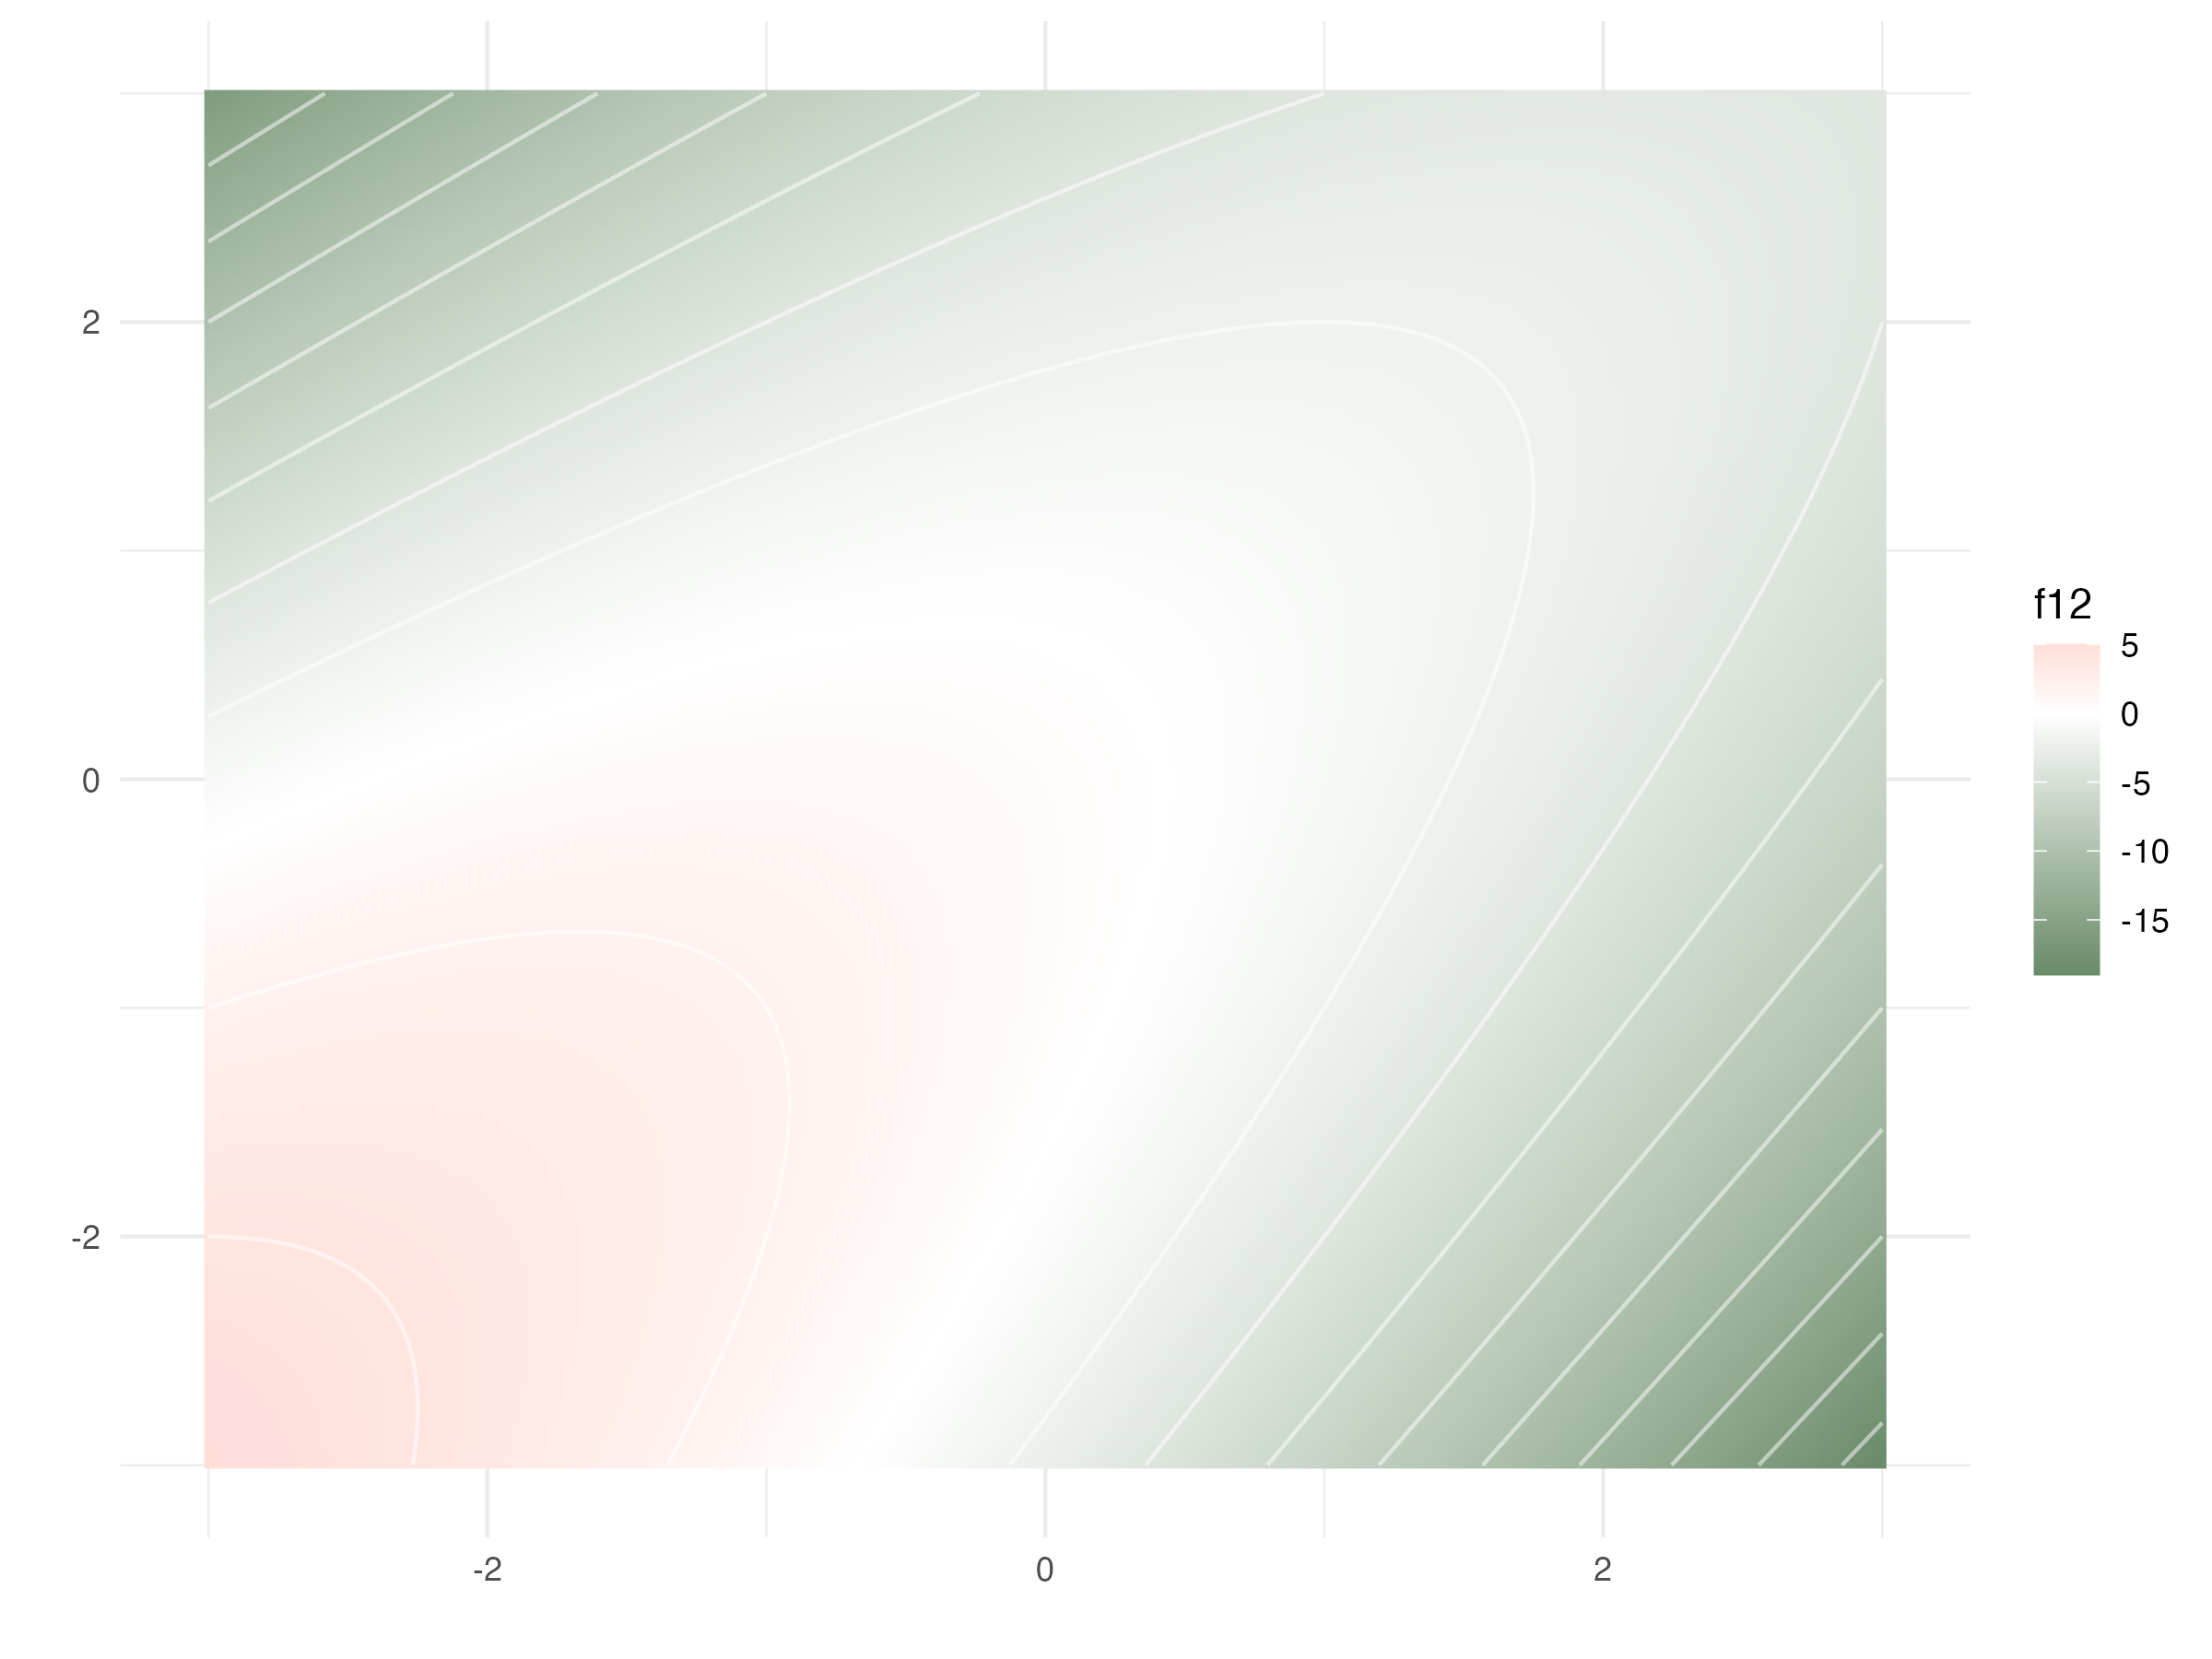
\includegraphics[width=\textwidth]{images/hoeffding_contour_rho05.png}
        \caption{Contour plot of $g(x) = x_1 + 2 x_2 + x_1 x_2$ with $\rho = 0.5$.}
        \label{fig:hoeffding_contour_rho05}
    \end{minipage}
\end{figure}
But the actualy fANOVA components are given by:
\begin{align*}
y_0 &= 0.5 \\[3pt]
y_1(x_1) &= x_1 + 0.4\,(x_1^2 - 1)
        = x_1 + 0.4x_1^2 - 0.4 \\[3pt]
y_2(x_2) &= 2x_2 + 0.4\,(x_2^2 - 1)
        = 2x_2 + 0.4x_2^2 - 0.4 \\[3pt]
y_{12}(x_1,x_2) 
&= -\Big( 0.4(x_1^2 + x_2^2) - x_1 x_2 - 0.3 \Big) \\[3pt]
&= -0.4x_1^2 - 0.4x_2^2 + x_1 x_2 + 0.3.
\end{align*}
These are visualized in \autoref{fig:dep_150_main} and \autoref{fig:dep_150_interact}.
% Input: MVN, dependent, rho = 0.5
\begin{figure}[htpb]
    \centering
    \begin{minipage}[t]{0.49\textwidth}
        \centering
        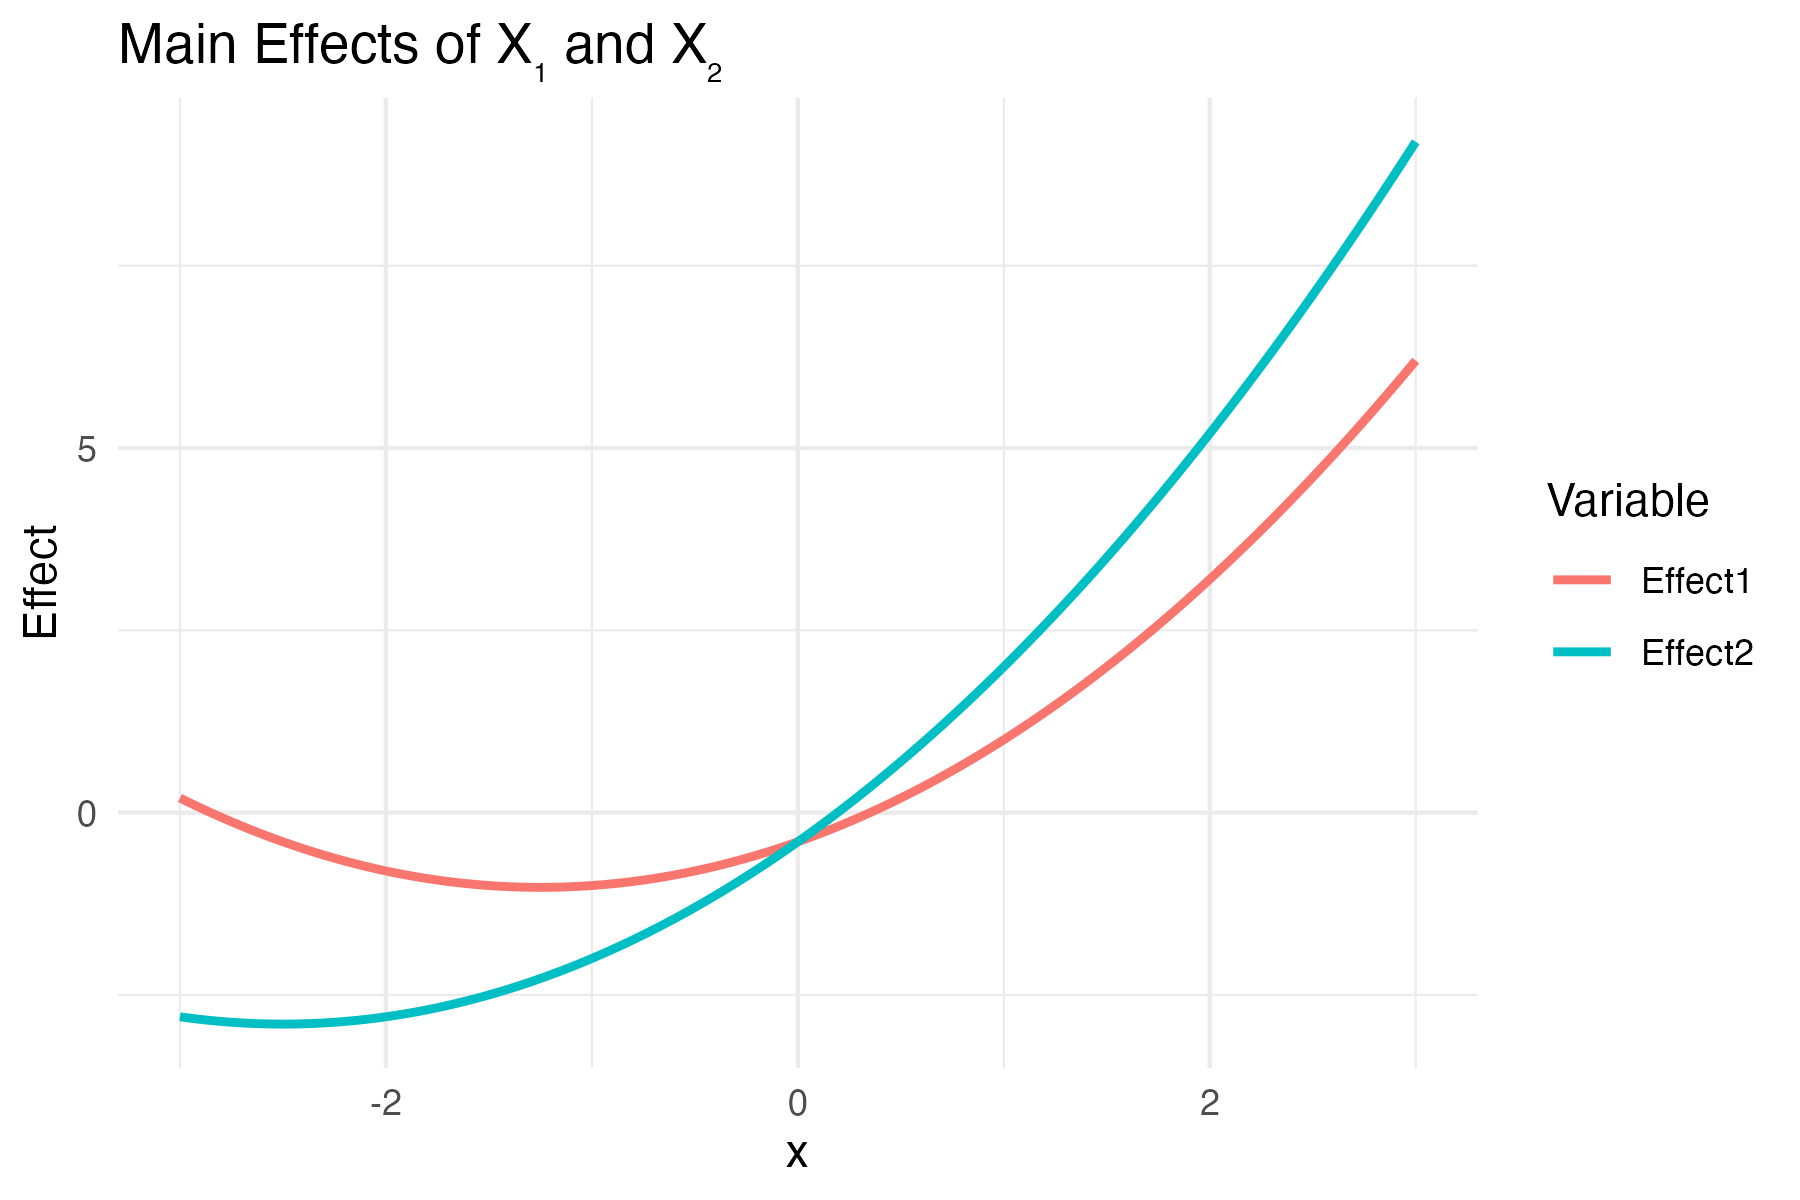
\includegraphics[width=\textwidth]{images/running_ex_a1p10_a2p20_a11p00_a22p00_a12p10_rhop05_main.png}
        \caption{Generalized main effects for $g(x) = x_1 + 2 x_2 + x_1 x_2$ with dependent inputs, $\rho = 0.5$.}
        \label{fig:dep_150_main}
    \end{minipage}%
    \hfill
    \begin{minipage}[t]{0.49\textwidth}
        \centering
        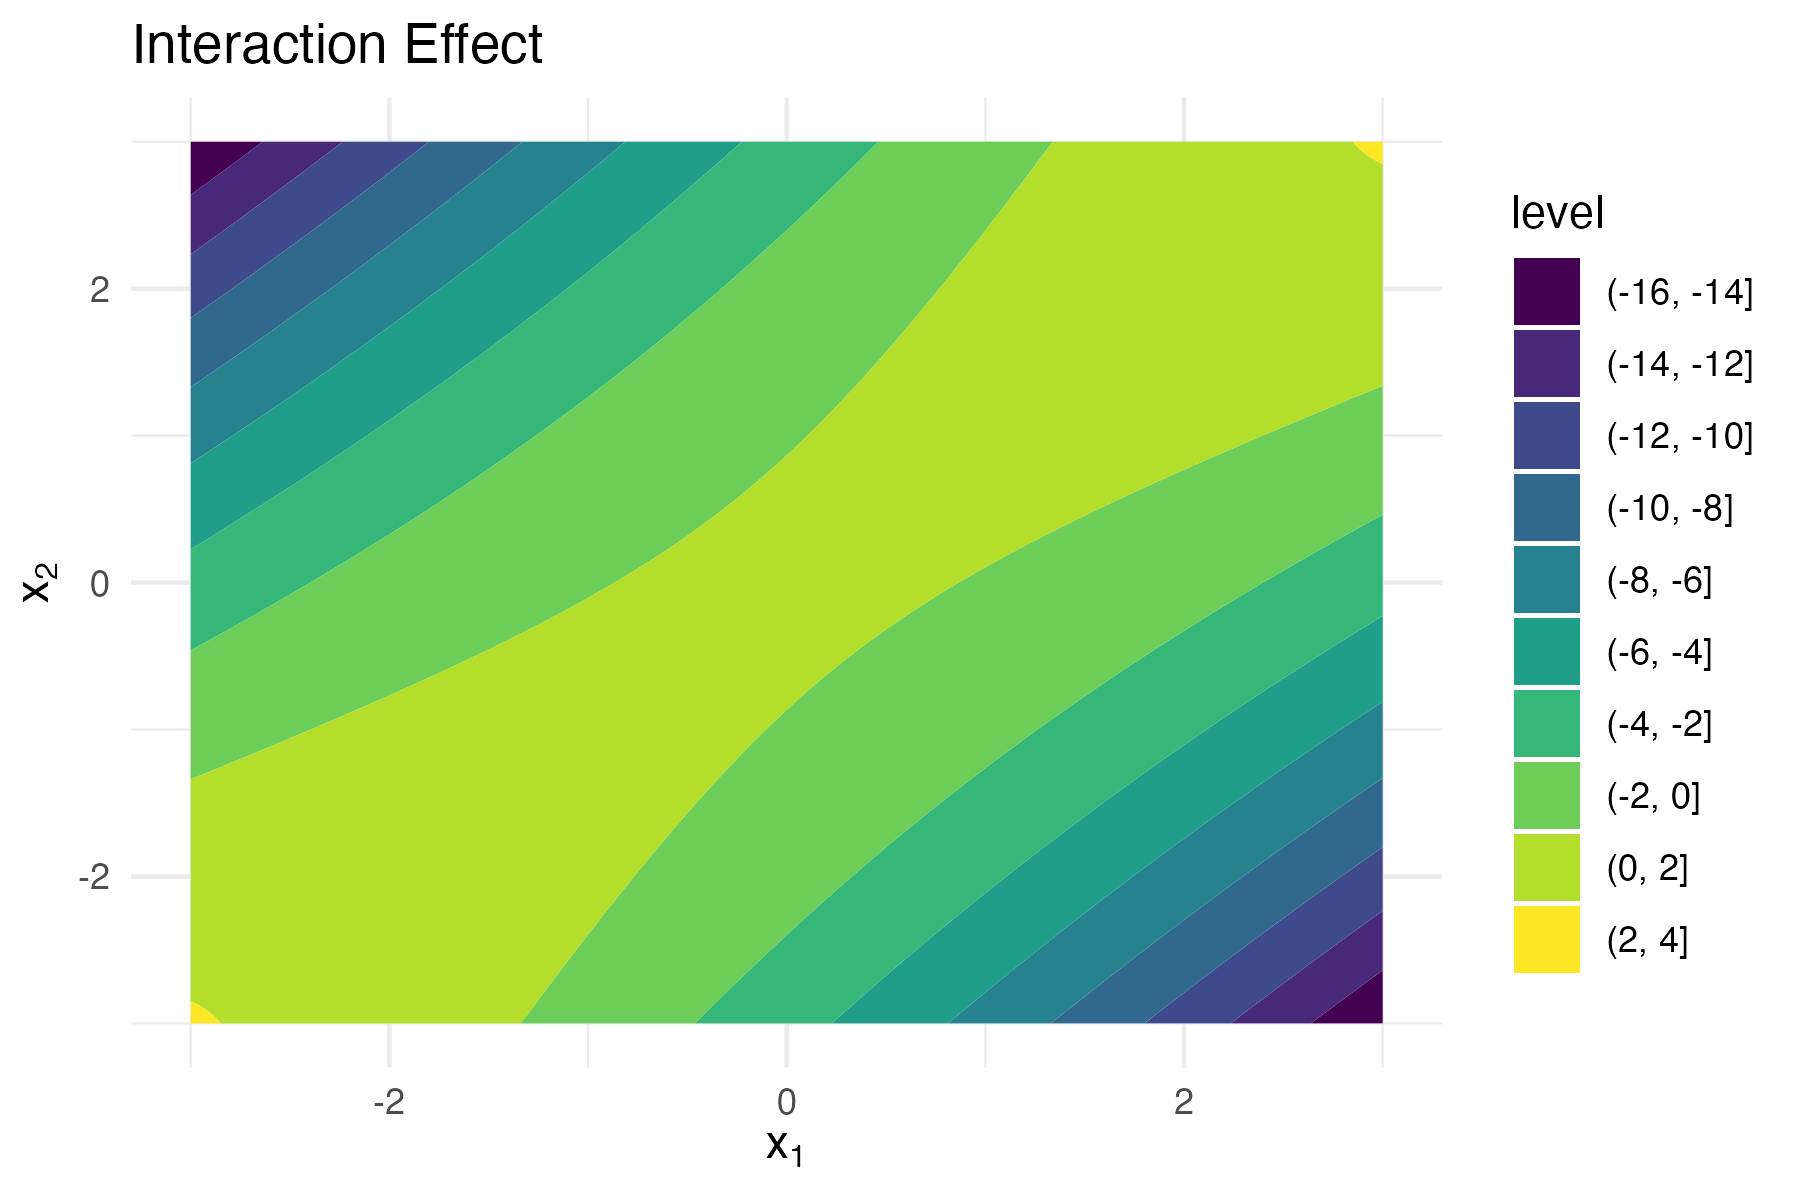
\includegraphics[width=\textwidth]{images/running_ex_a1p10_a2p20_a11p00_a22p00_a12p10_rhop05_interaction.png}
        \caption{Contour plot of generalized interaction term for $g(x) = x_1 + 2 x_2 + x_1 x_2$ with dependent inputs, $\rho = 0.5$.}
        \label{fig:dep_150_interact}
    \end{minipage}
\end{figure}
Interestingly, the parabolic form of the main effects is similar between Hoeffding and fANOVA, but the interaction effects diverge notably.\par
Our running example included linear effects of both input variables and the interaction term. For the remainder of this section, we will explore other representative scenarios, we can build within the scaffold of a bivariate two degree polynomial.

\subsection{Comparison of Functions}
\subsubsection*{Scenario: Linear}
First, we consider two-degree polynomials of the form:
$$g_1(x_1, x_2) = a_1 x_1 + a_2 x_2.$$
We are interested in examining how the fANOVA components change for different values of the coefficients $a_1$ and $a_2$. 
Since an interaction effect is absent in $g_1$, the fANOVA interaction term is also zero and varying $\rho$ or visualizing an interaction term is of no interest.
\begin{figure}[htpb]
    \centering
    \begin{minipage}[t]{0.49\textwidth}
        \centering
        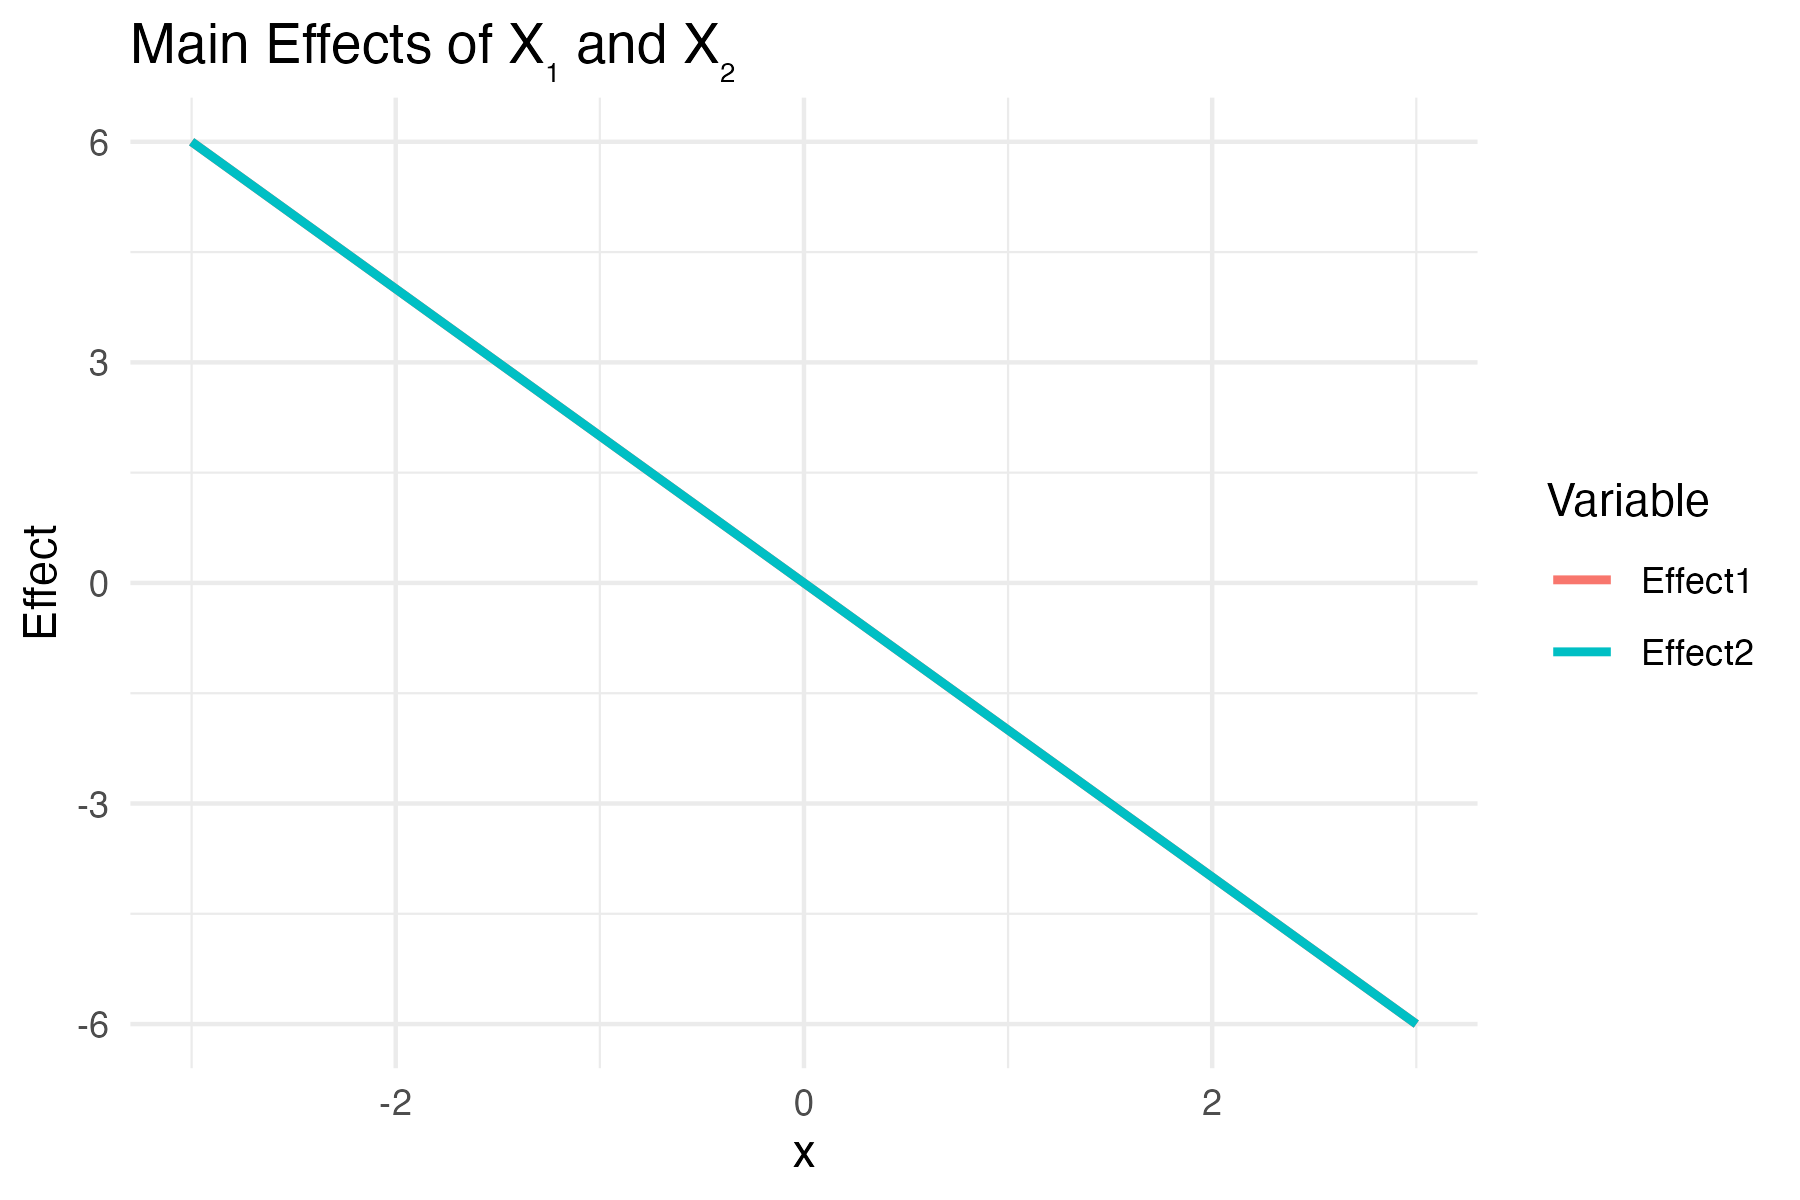
\includegraphics[width=\textwidth]{images/linear_a1m20_a2m20_a11p00_a22p00_a12p00_rhop00_main.png}
    \end{minipage}%
    \hfill
    \begin{minipage}[t]{0.49\textwidth}
        \centering
        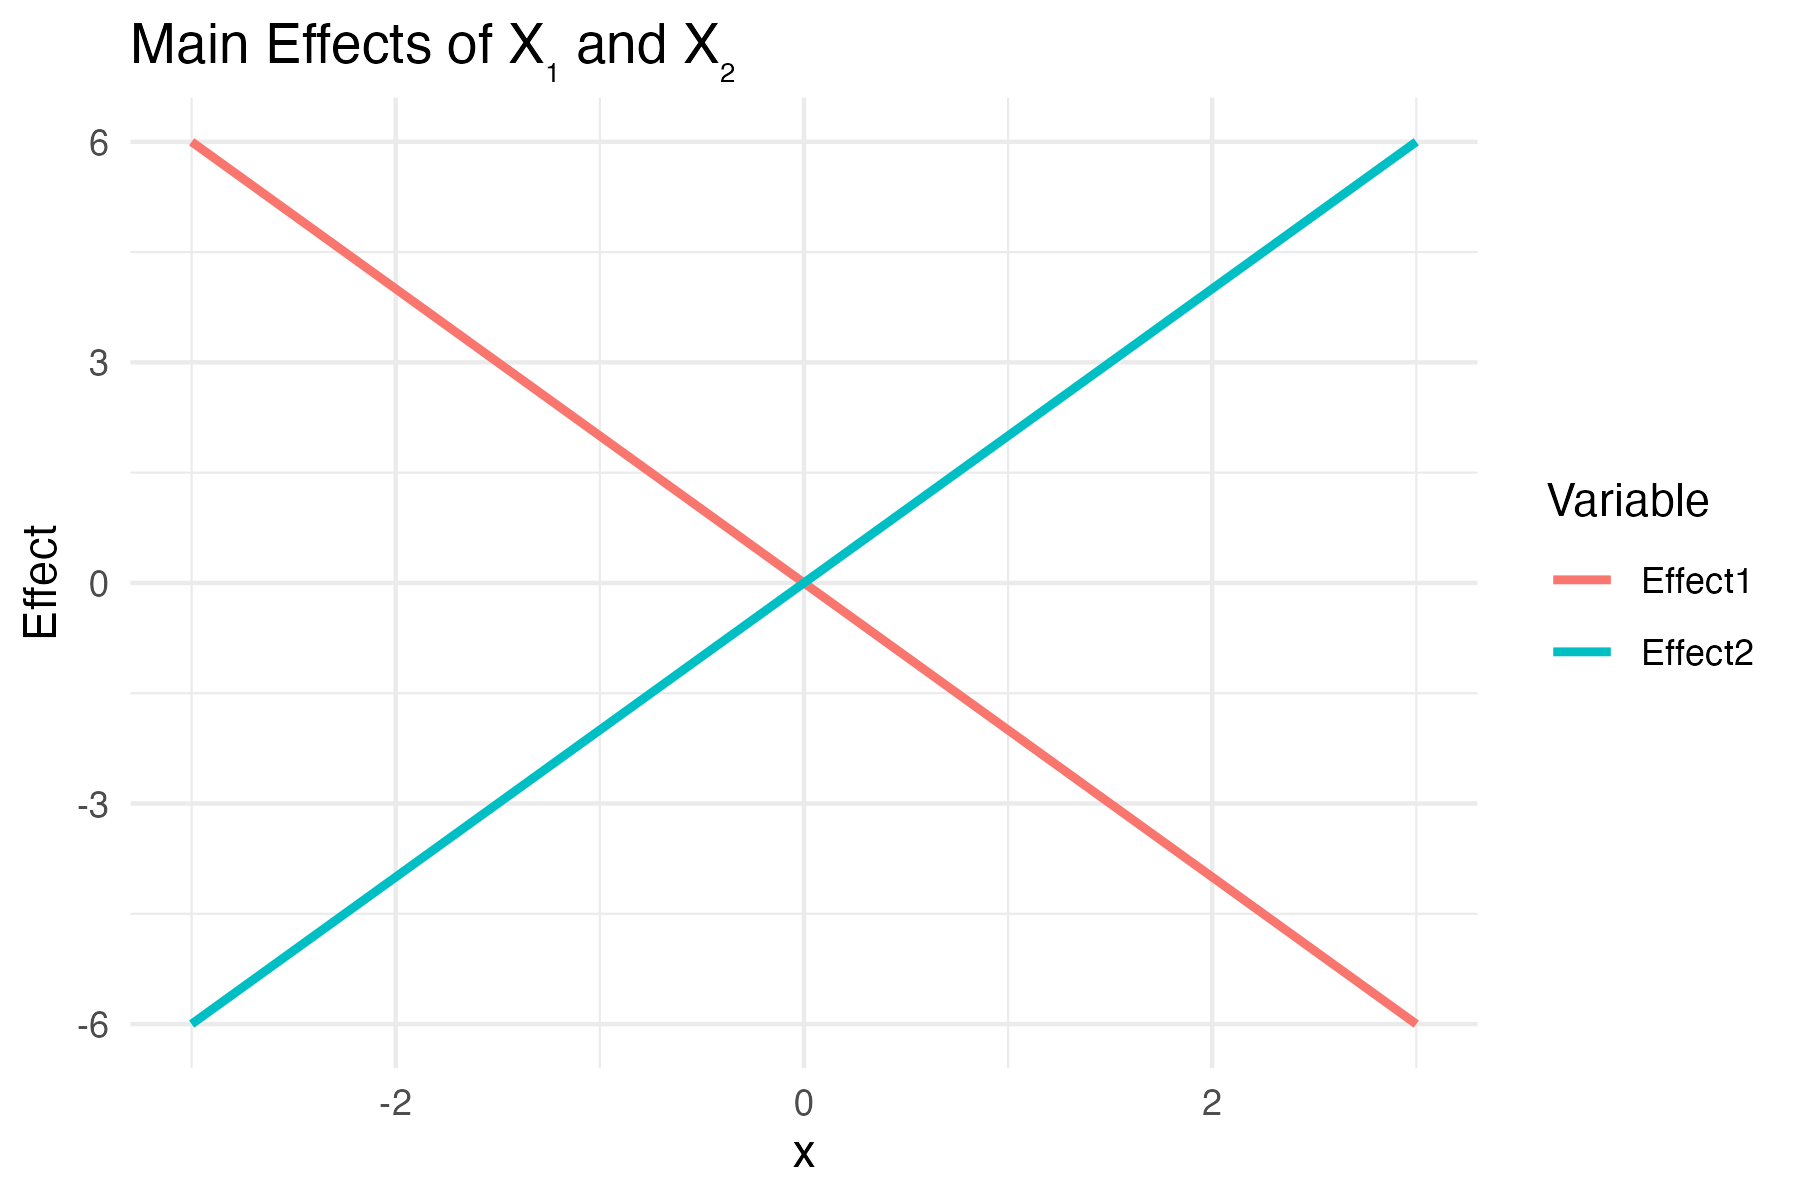
\includegraphics[width=\textwidth]{images/linear_a1m20_a2p20_a11p00_a22p00_a12p00_rhop00_main.png}
    \end{minipage}
    \caption{Main fANOVA components for linear terms with different coefficients.\textbf{ Left:} $y_1(x_1) = -2x_1$, $y_2(x_2) = -2x_2$.\textbf{ Right:} $y_1(x_1) = -2x_1$, $y_2(x_2) = 2x_2$.}
    \label{fig:linear_main_effects}
\end{figure}



\subsubsection*{Scenario: Quadratic}
Next we consider two-degree polynomials, which contain only quadratic terms; they take the form: $$g_2(x_1, x_2) = a_{11} x_1^2 + a_{22} x_2^2.$$
As for the linear scenario, we vary the coefficients $a_{11}$ and $a_{22}$, while the interaction term is absent. We observe the same ``symmetric'' pattern as in the linear case.
\begin{figure}[htpb]
    \centering
    \begin{minipage}[t]{0.49\textwidth}
        \centering
        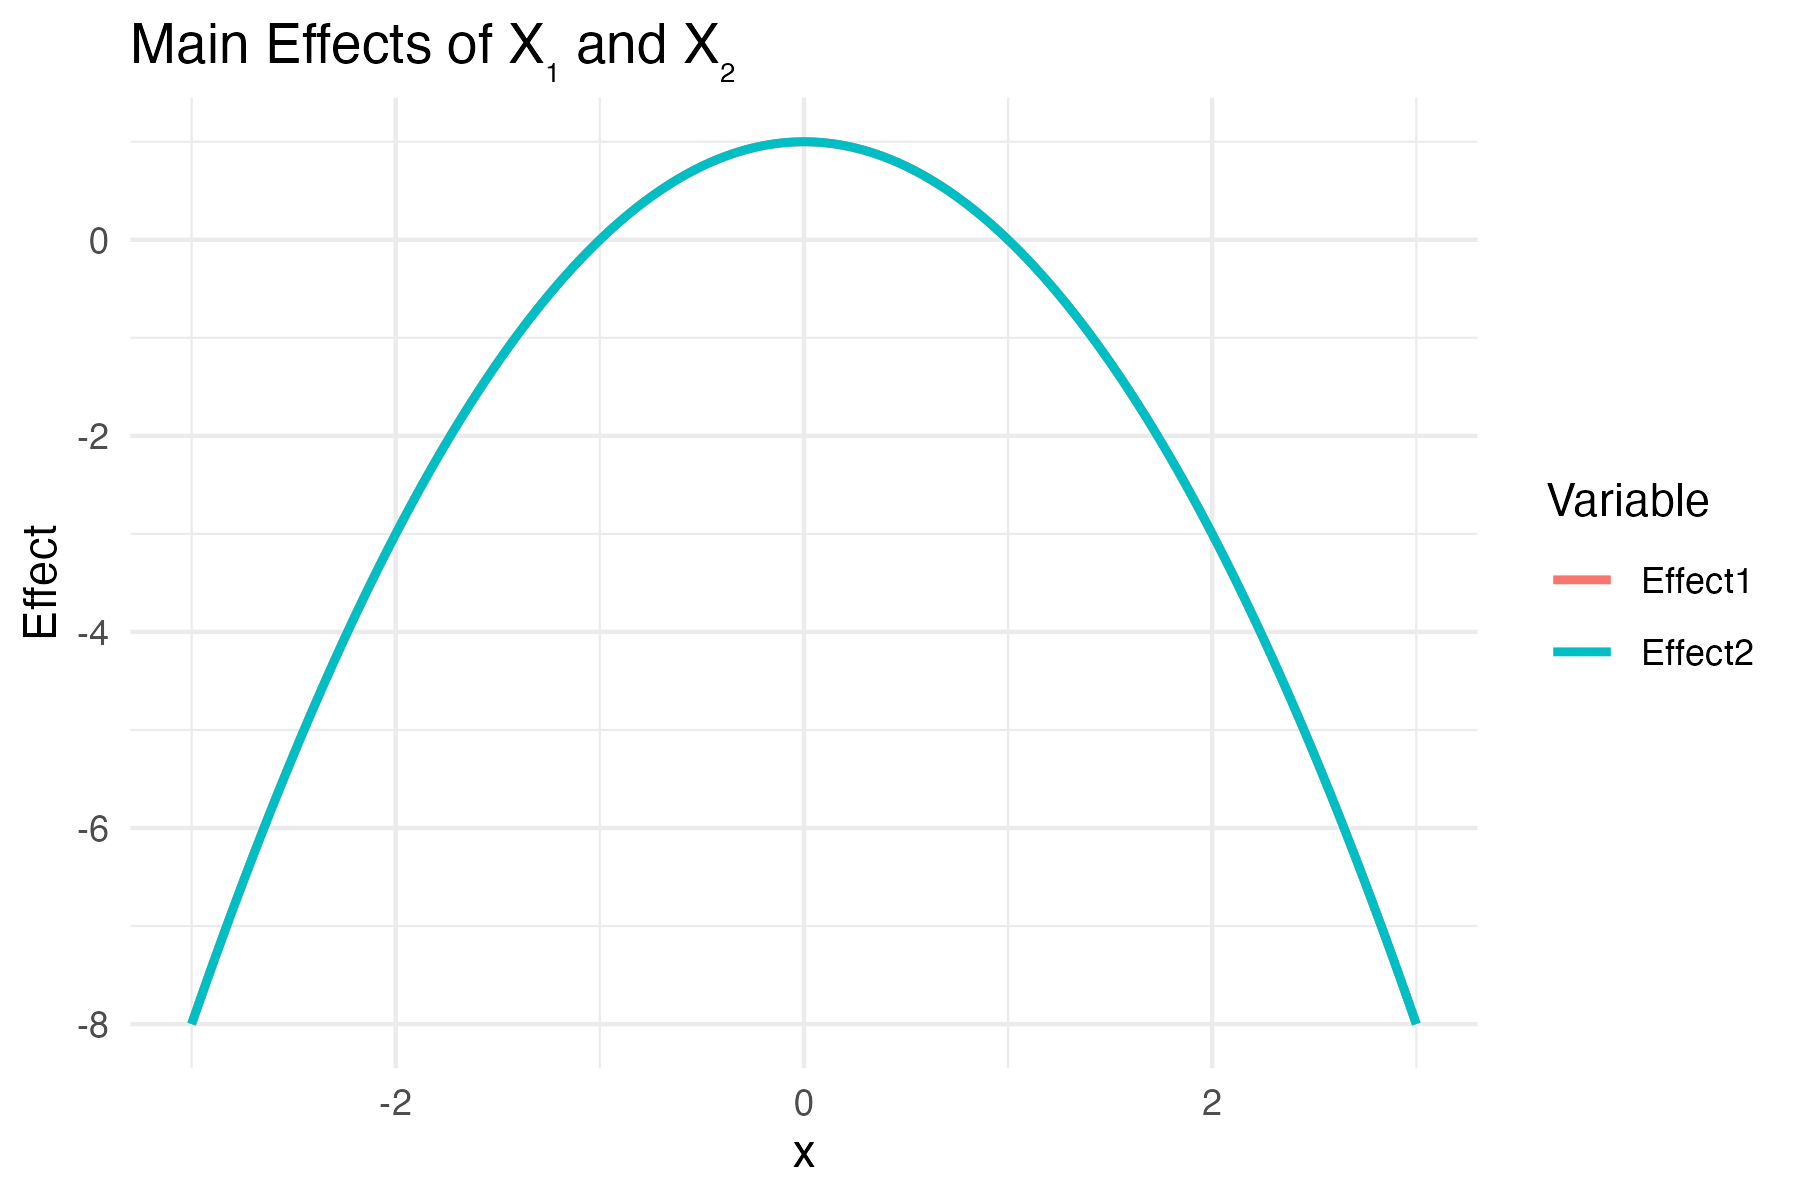
\includegraphics[width=\textwidth]{images/quadratic_a1p00_a2p00_a11m10_a22m10_a12p00_rhop00_main.png}
    \end{minipage}%
    \hfill
    \begin{minipage}[t]{0.49\textwidth}
        \centering
        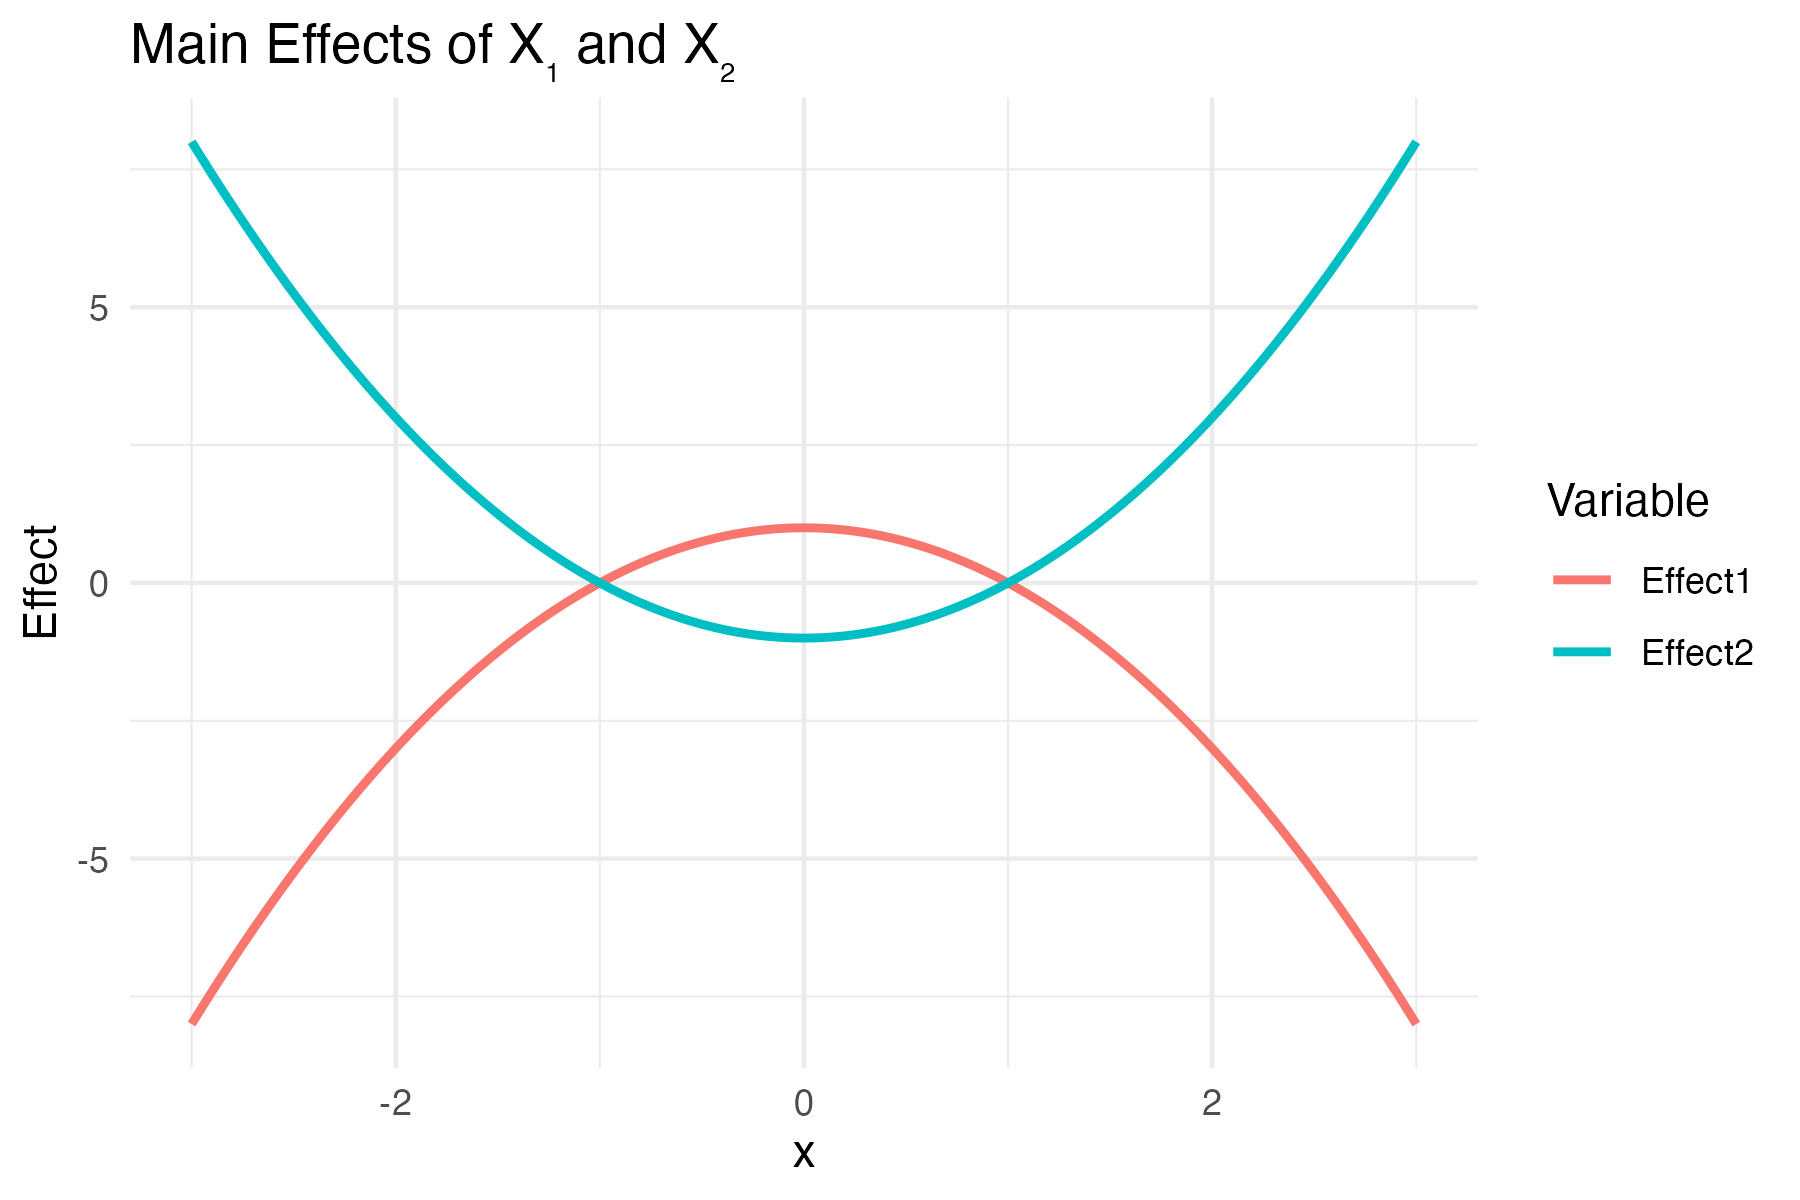
\includegraphics[width=\textwidth]{images/quadratic_a1p00_a2p00_a11m10_a22p10_a12p00_rhop00_main.png}
    \end{minipage}
    \caption{
        Main effects for quadratic terms with different coefficients. 
        \textbf{Left:} $y_0 = -2$, $y_1(x_1) = -1(x_1^2 - 1)$, $y_2(x_2) = -1(x_2^2 - 1)$. 
        \textbf{Right:} $y_1(x_1) = -1(x_1^2 - 1)$, $y_2(x_2) = 1(x_2^2 - 1)$.
    }
    \label{fig:quadratic_main_effects}
\end{figure}



\subsubsection*{Scenario: Interaction only}
Next, we consider a model, which solely consists of an interaction term: $$g_3(x_1, x_2) = a_{12} x_1 x_2.$$
Here it is interesting to vary $\rho$, while we ignore varying the coefficients of the main effects, since they are absent. The interaction effect is plotted as a contour plot for varying $\rho$ with the corresponding main effects next to it.
In \autoref{fig:interaction_rho_neg05} we set $\rho = -0.5$, while in \autoref{fig:interaction_rho_1} we set $\rho = 1$. From this we can conclude, that the main effects for $g_3$ are only influenced by the sign of $\rho$, not its magnitude. So for the main effects, it suffices to distinguish between $\rho < 0$, $\rho = 0$, and $\rho > 0$. The interaction term is, of course, influenced by sign and magnitude of $\rho$.
\begin{figure}[htpb]
    \centering
    \begin{minipage}[t]{0.49\textwidth}
        \centering
        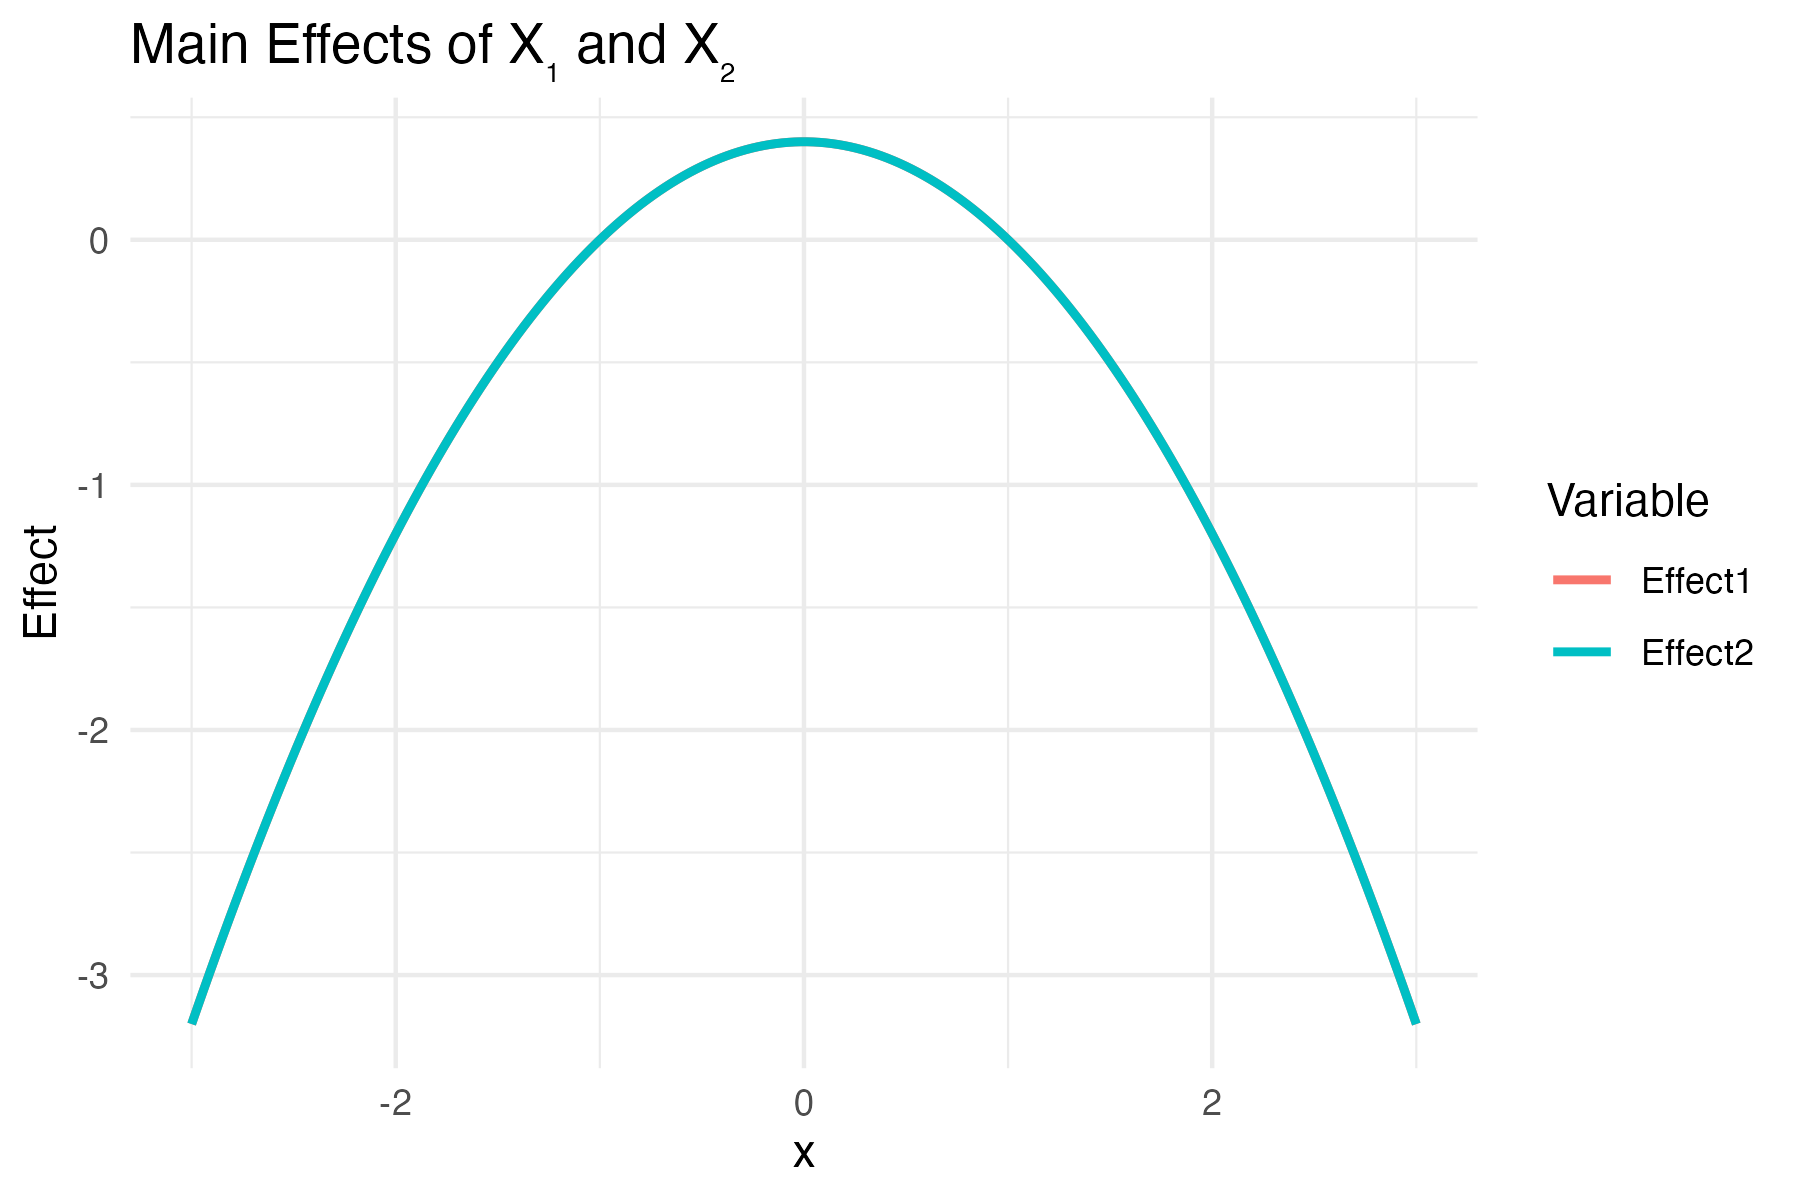
\includegraphics[width=\textwidth]{images/interaction_a1p00_a2p00_a11p00_a22p00_a12p10_rhom05_main.png}
    \end{minipage}%
    \hfill
    \begin{minipage}[t]{0.49\textwidth}
        \centering
        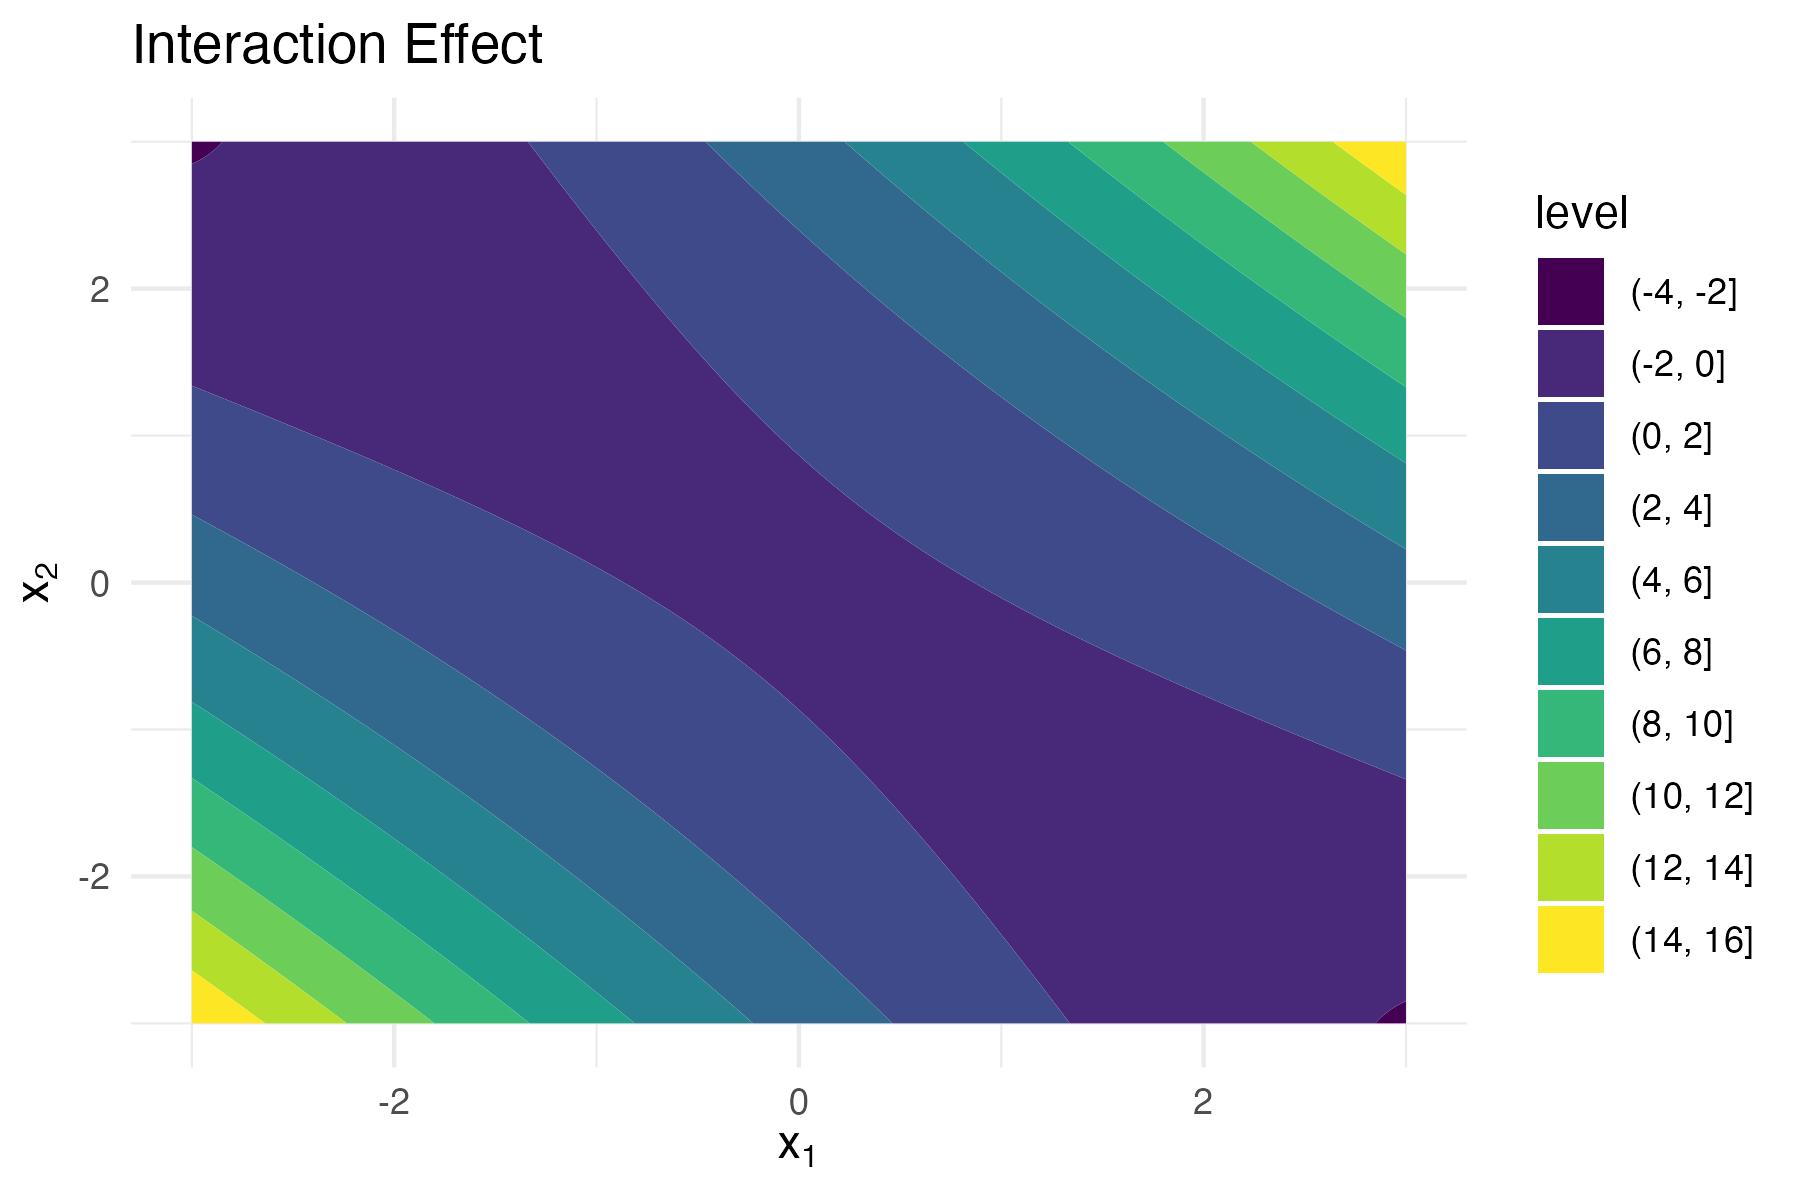
\includegraphics[width=\textwidth]{images/interaction_a1p00_a2p00_a11p00_a22p00_a12p10_rhom05_interaction.png}
    \end{minipage}
    \caption{Main effects and contour plot of interaction effects for $\rho = -0.5$}
    \label{fig:interaction_rho_neg05}
\end{figure}
\begin{align*}
y_0 &= -0.5 \\[3pt]
y_{12}(x_1,x_2) &= 0.4x_1^2 + 0.4x_2^2 + x_1x_2 - 0.3
\end{align*}


\begin{figure}[htpb]
    \centering
    \begin{minipage}[t]{0.49\textwidth}
        \centering
        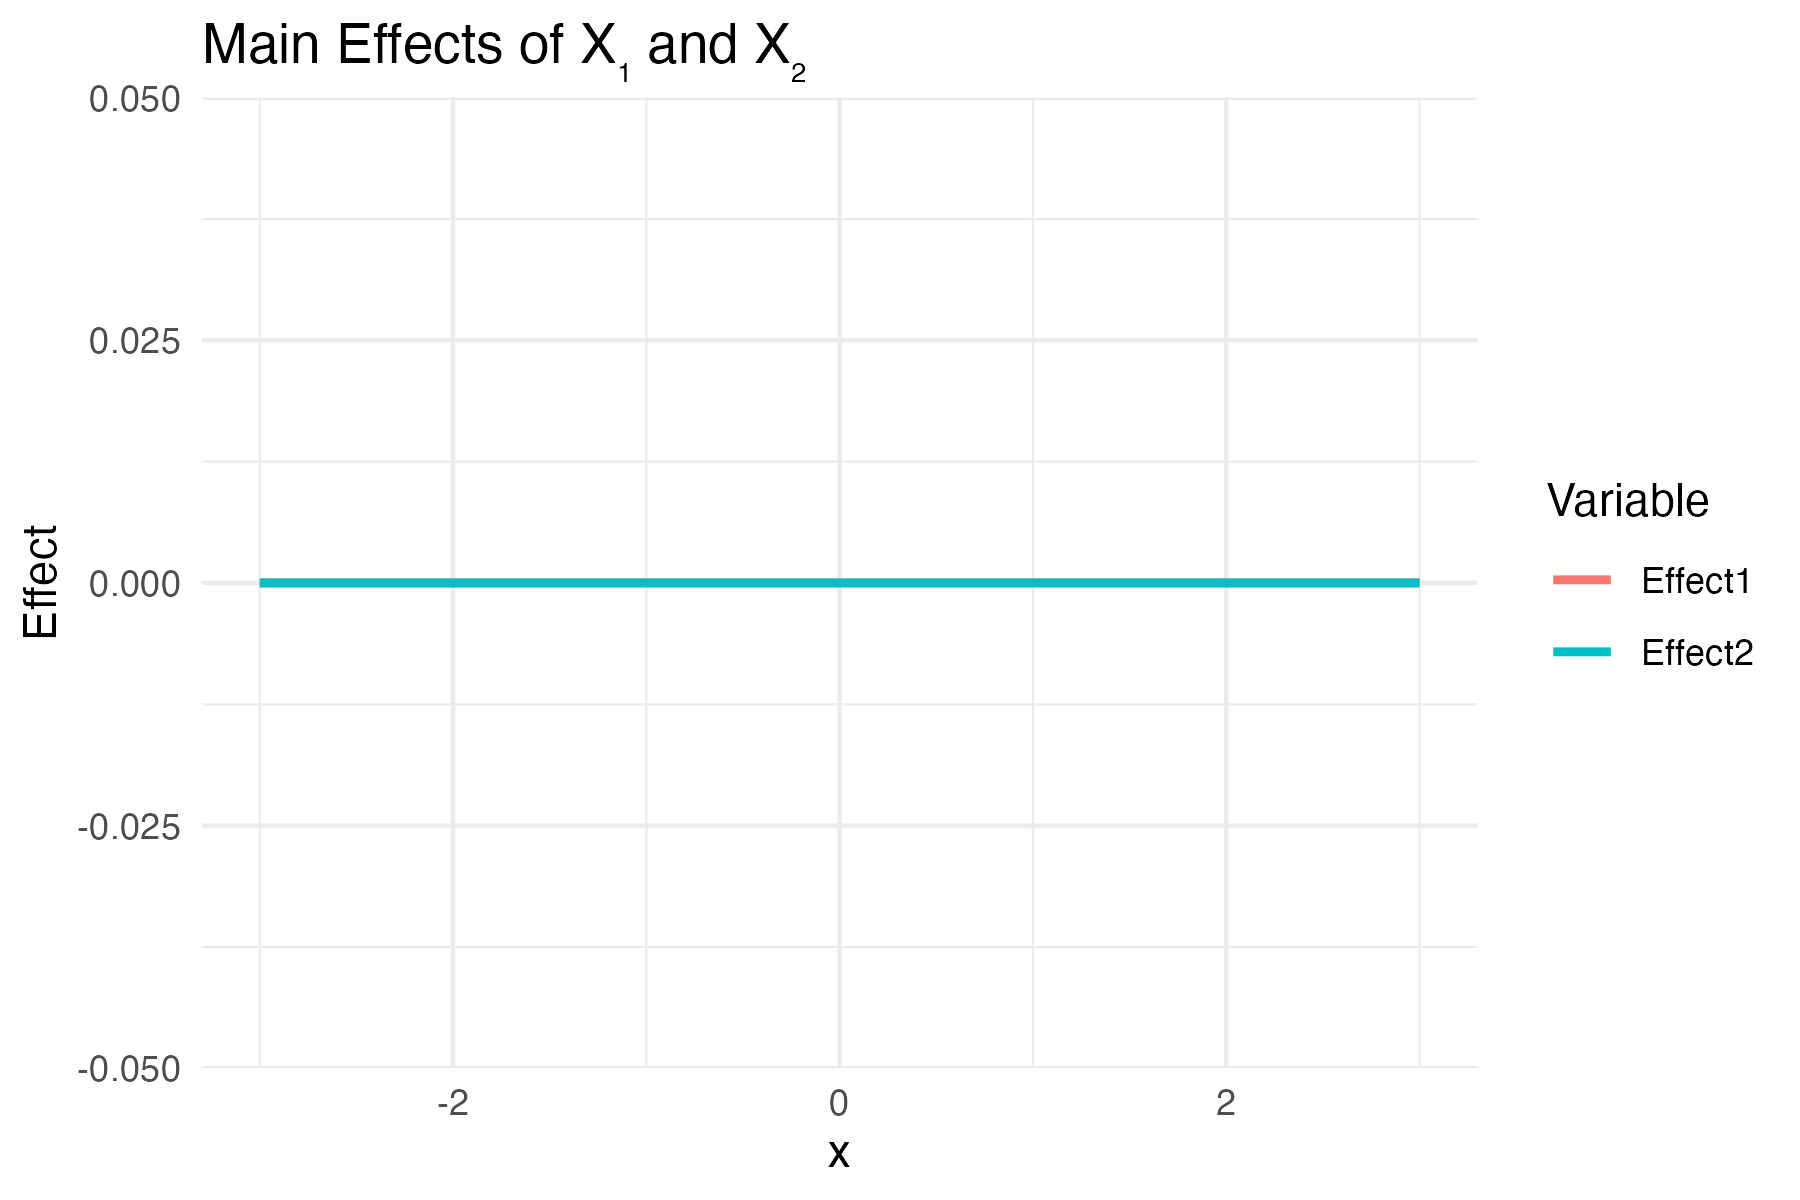
\includegraphics[width=\textwidth]{images/interaction_a1p00_a2p00_a11p00_a22p00_a12p10_rhop00_main.png}
    \end{minipage}%
    \hfill
    \begin{minipage}[t]{0.49\textwidth}
        \centering
        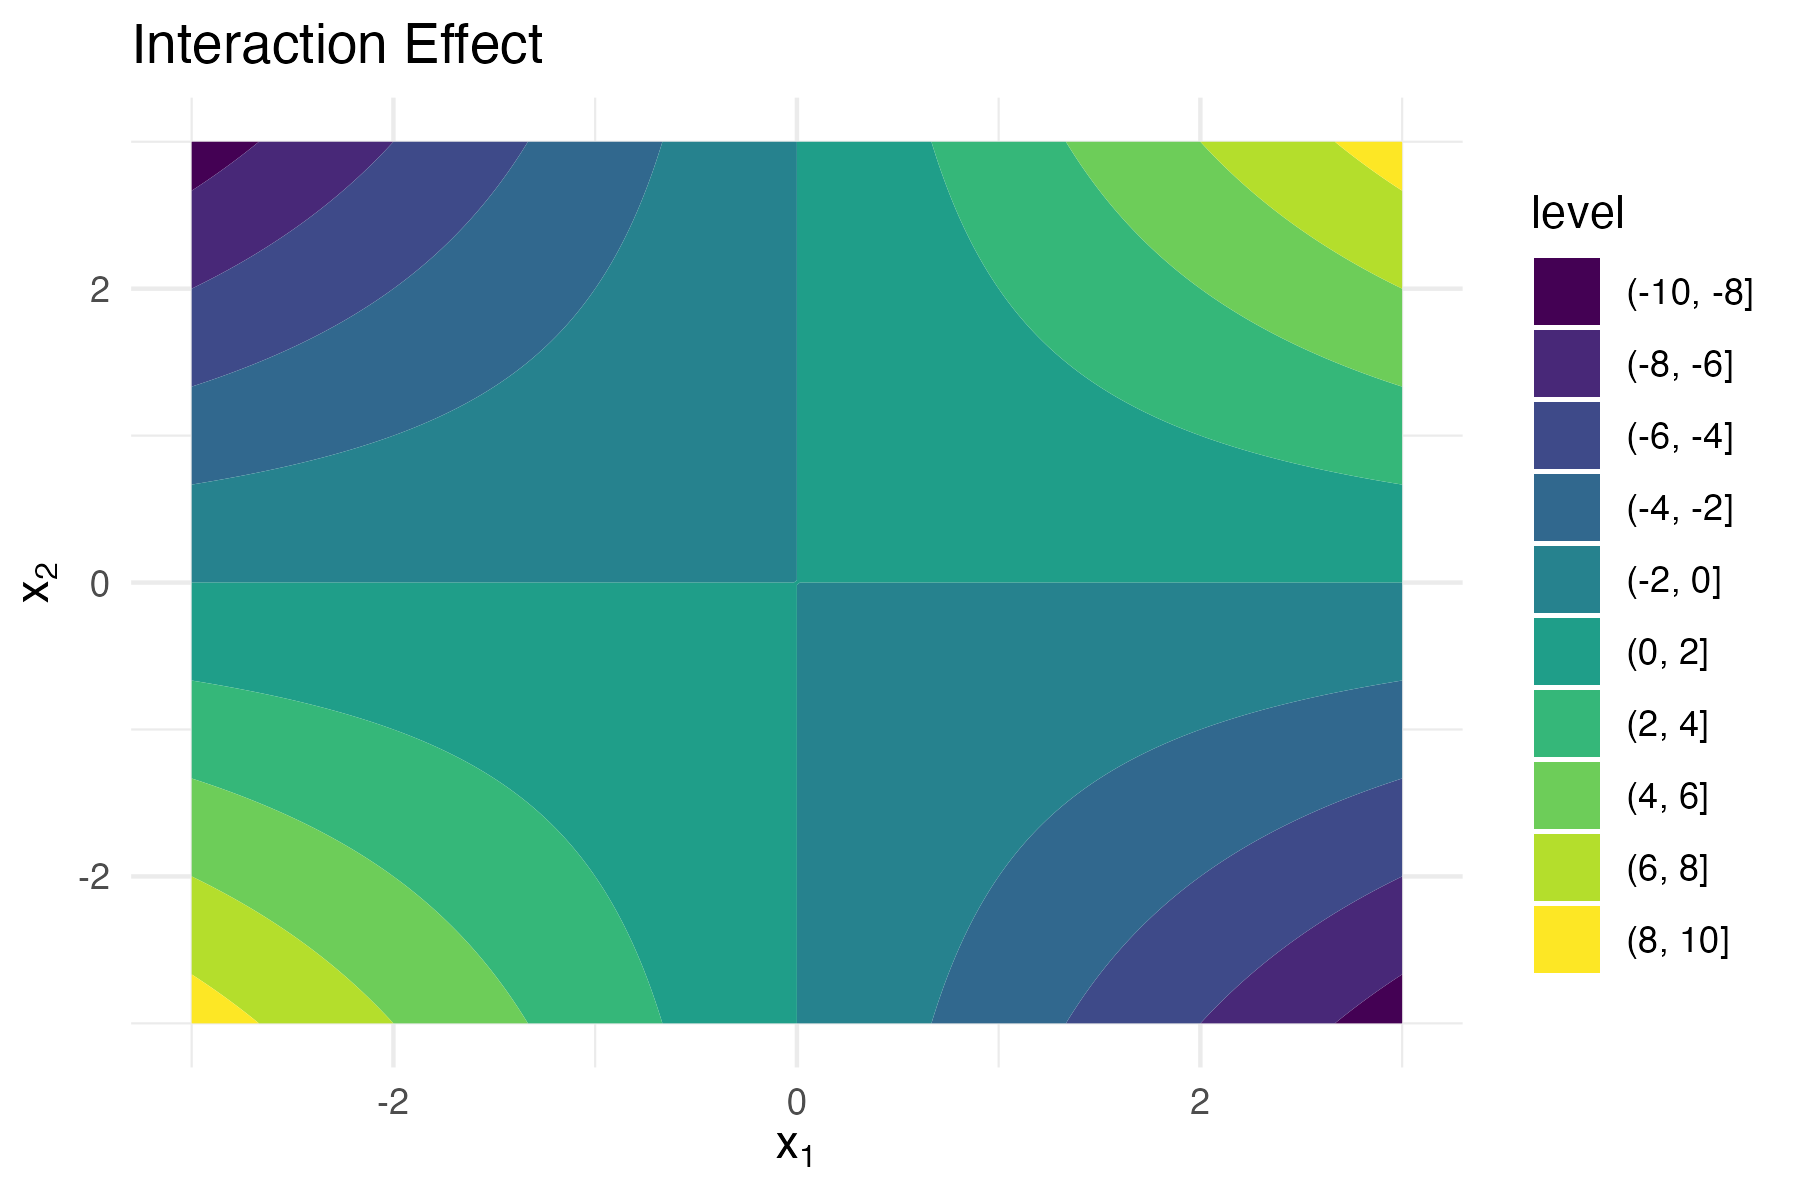
\includegraphics[width=\textwidth]{images/interaction_a1p00_a2p00_a11p00_a22p00_a12p10_rhop00_interaction.png}
    \end{minipage}
    \caption{Main effects and contour plot of interaction effects for $\rho = 0$}
    \label{fig:interaction_rho_0}
\end{figure}
\begin{align*}
y_{12}(x_1,x_2) &= x_1x_2
\end{align*}


\begin{figure}[htpb]
    \centering
    \begin{minipage}[t]{0.49\textwidth}
        \centering
        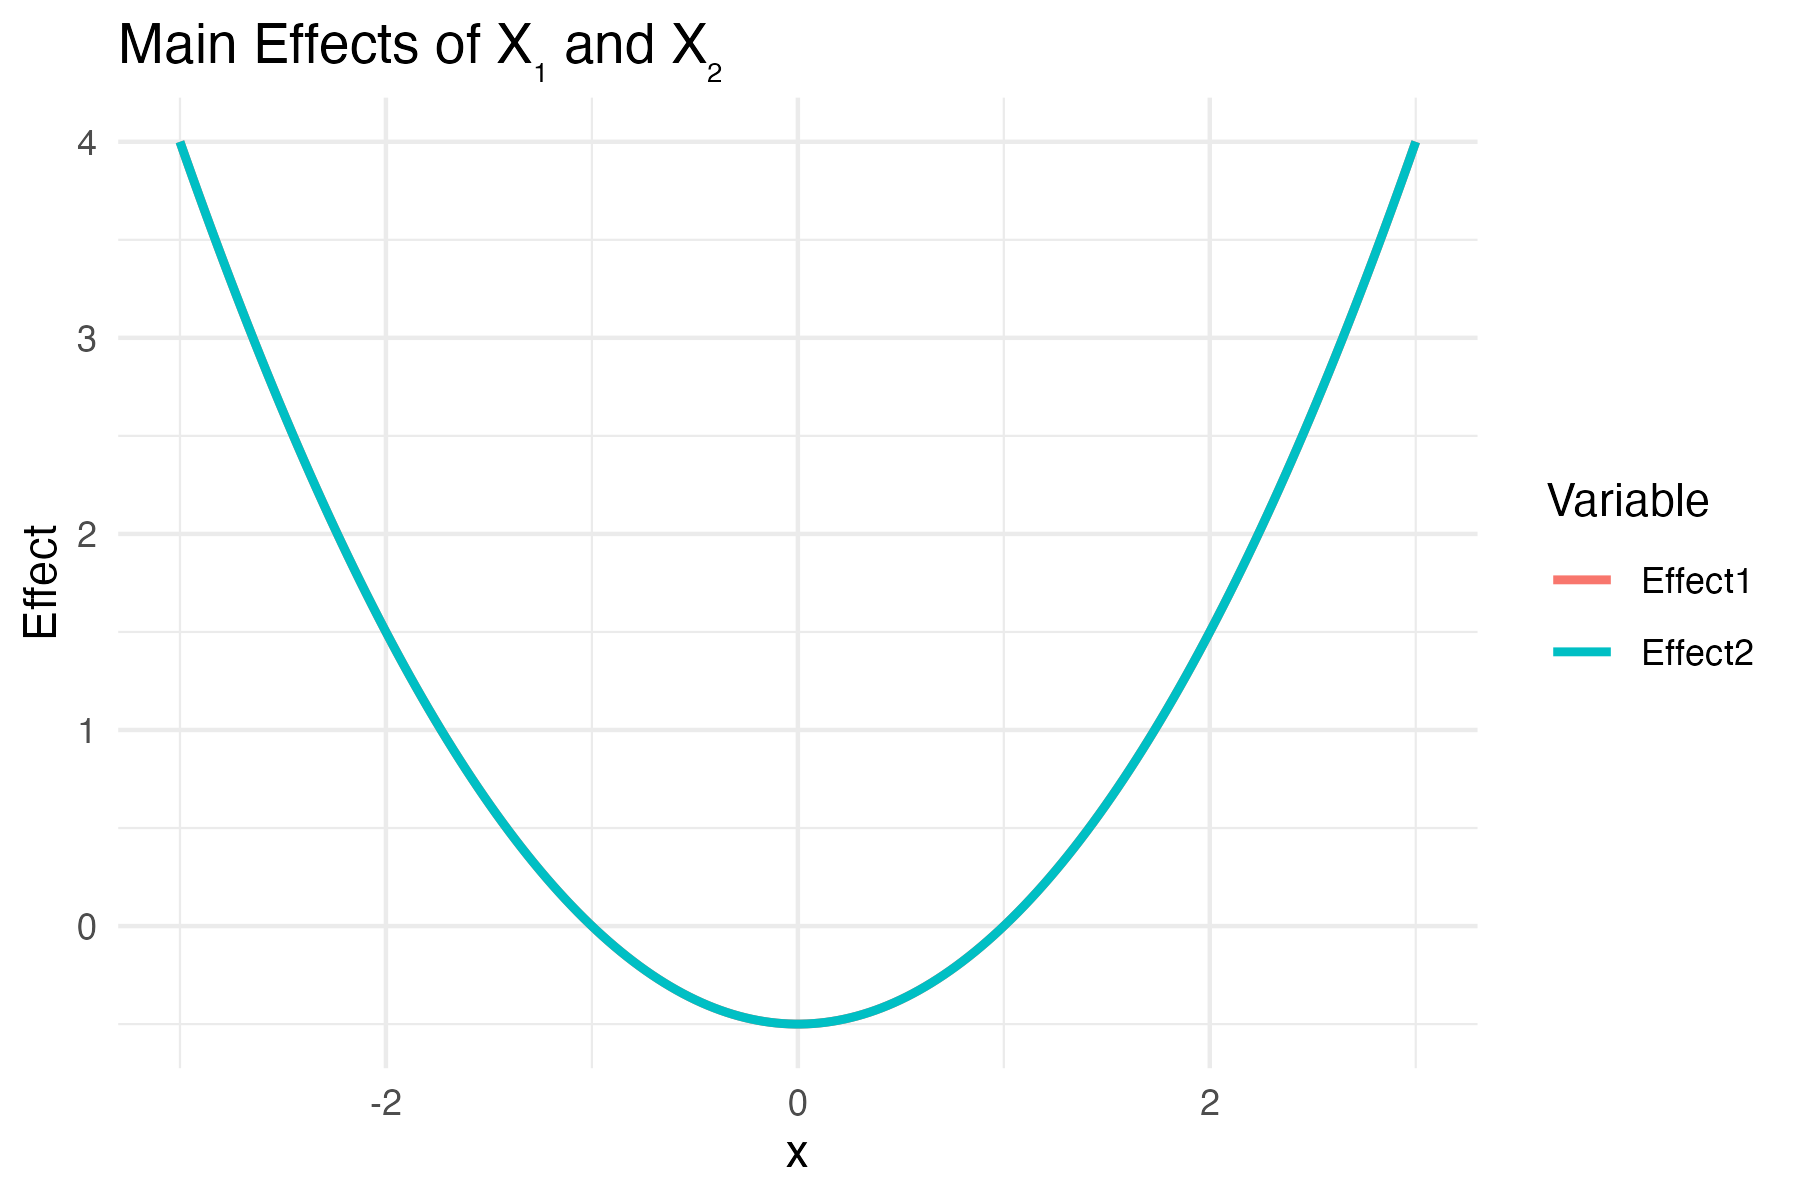
\includegraphics[width=\textwidth]{images/interaction_a1p00_a2p00_a11p00_a22p00_a12p10_rhop10_main.png}
    \end{minipage}%
    \hfill
    \begin{minipage}[t]{0.49\textwidth}
        \centering
        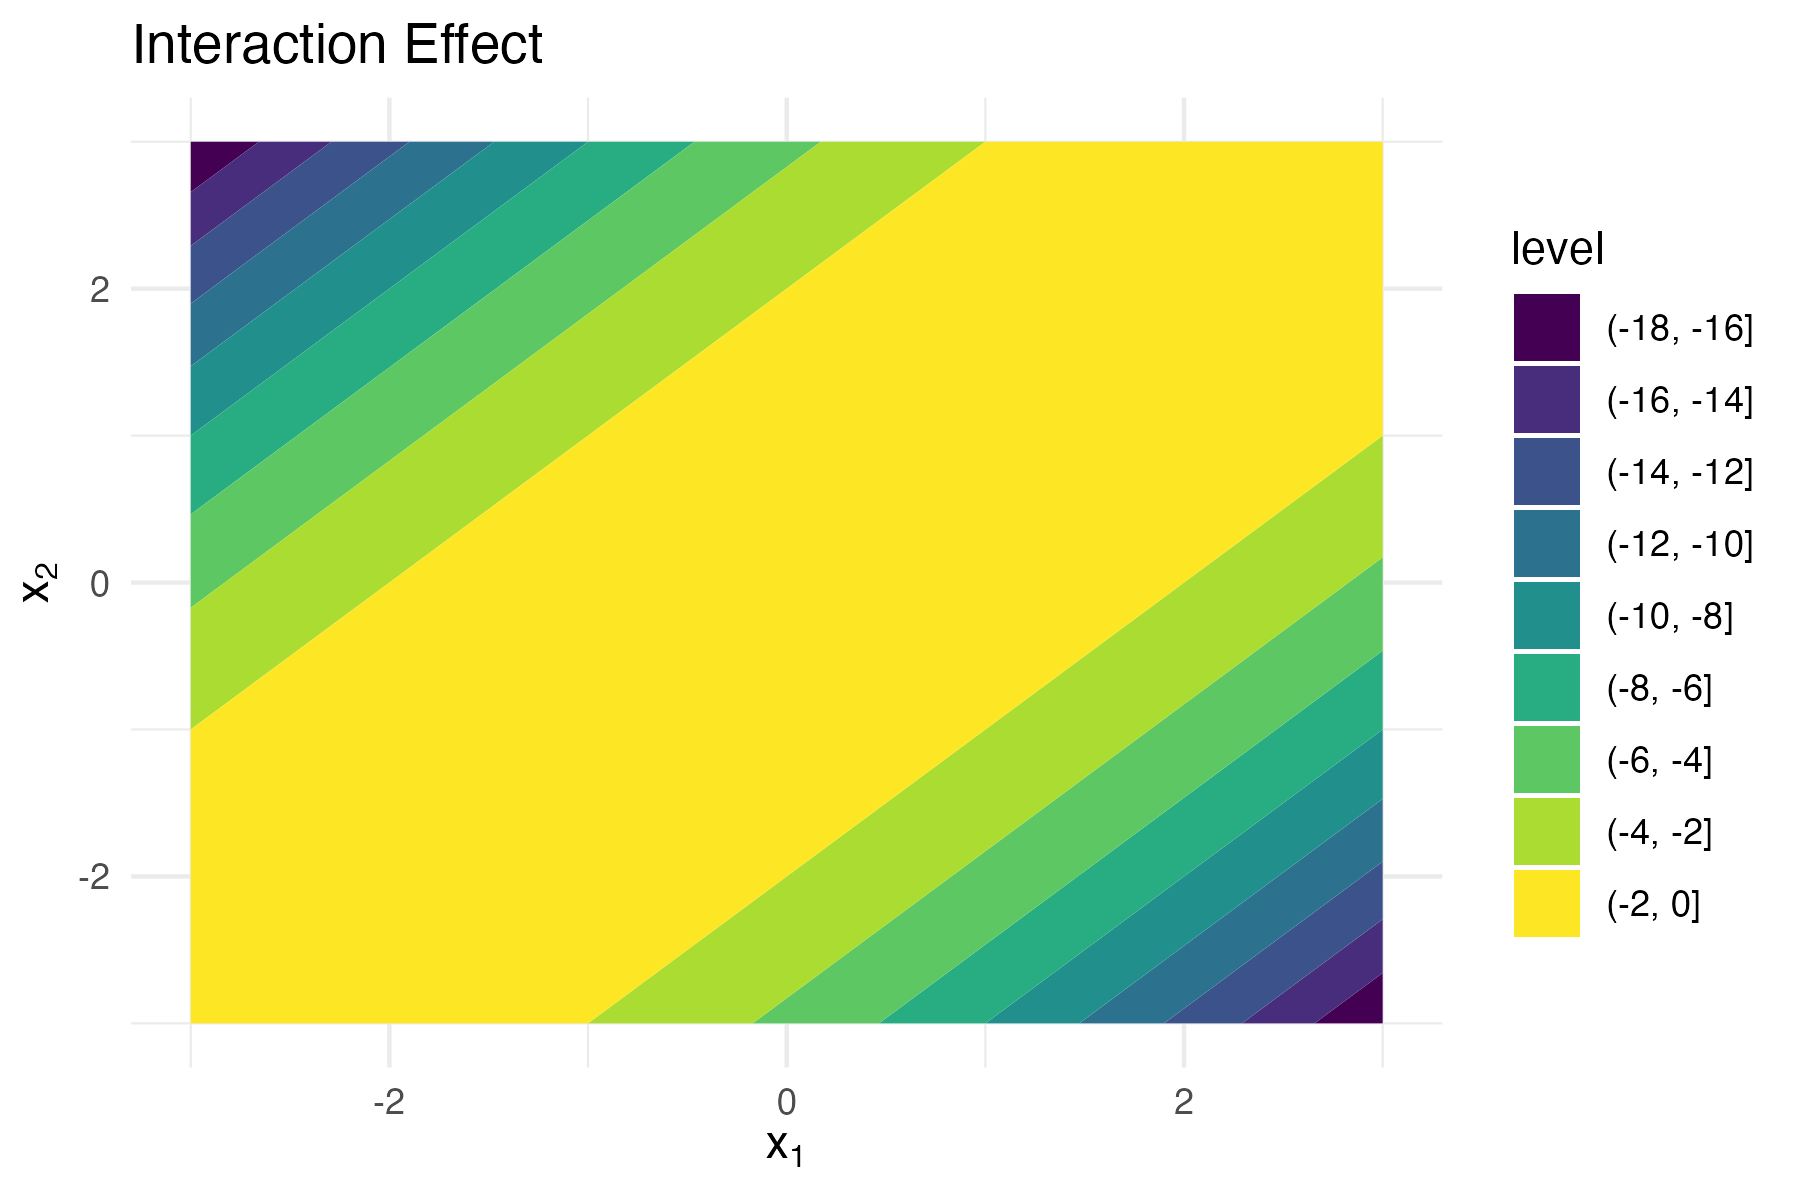
\includegraphics[width=\textwidth]{images/interaction_a1p00_a2p00_a11p00_a22p00_a12p10_rhop10_interaction.png}
    \end{minipage}
    \caption{Main effects and contour plot of interaction effects for $\rho = 1$}
    \label{fig:interaction_rho_1}
\end{figure}
\begin{align*}
y_0 &= 1 \\[3pt]
y_{12}(x_1,x_2) &= -0.5x_1^2 - 0.5x_2^2 + x_1x_2
\end{align*}


\subsubsection*{Scenario: Mixed, only main}
Following, we study the main effects of two-degree polynomials, which allow for effects of linear and quadratic nature:
\[
g_4(x_1, x_2) = a_1 x_1 + a_2 x_2 + a_{11} x_1^2 + a_{22} x_2^2,
\]
so we vary the coefficients again but not $\rho$.
The shape of the parabolas in the upper left panel is representative of cases, where the coefficients of the linear terms $a1$ and $a2$ have the same sign and the ones of the quadratic terms $a11$ and $a22$ have the same sign.
The coefficients of the quadratic terms $a11$ and $a22$ determine whether the parapbola is facing downwards or upwards/ open upwards or downwards; when they are both negative the parabola is open downwards and when they are both positive the parabola is upwards open. The linear coefficients $a1$ and $a2$ determine how stretched or compressed the parabola is.\par
The upper right plot and the lower left plot show typical behviour for cases where the quadratic coefficients have different signs. In such cases we get parabolas that are open in opposite directions. The only systematic difference between the upper right and lower left is that within variable sign-difference is only true for one variable, either $X_1$ or $X_2$ in the lower left plot.\par
Lastly, in the lower right we have cases where we have again within variable sign difference, but the signs of the quadratic coefficients are the same. Here we have a symmetric pattern, where the parabolas are open in the same direction.

% The upper right plot is representative of cases where we have within-variable sign difference and a symmetric between variable sign-difference, for example we look at cases such as $a1 = -2, a11 = 1, a2 = 2, a22 = -1$ or $a1 = 2, a11 = -1, a2 = -2, a22 = 1$. Here again, whether the parabola for a variable is facing upwards or downwards is determined by the sign of the quadratic coefficient.
% In the lower left we represent cases in which within-variable sign difference is only true for one variable, either $X_1$ or $X_2$, and the quadratic coefficients are sign-different. Then we get parabolas that are open in opposite directions.\par
% where we have 1. the same sign \textit{within} a variable and where we have 2. different signs \textit{within} a variable, but they are different in the same way for both variables. 1. includes sets of coefficients like
% $a1 = -2, a11 = -1, a2 = -2, a22 = -1$. 2. includes sets of coefficients like $a1 = 2, a11 = -1, a2 = 2, a22 = -1$ or $a1 = -2, a11 = -1, a2 = -2, a22 = 1$.

\begin{figure}[htpb]
    \centering
    \begin{minipage}[t]{0.49\textwidth}
        \centering
        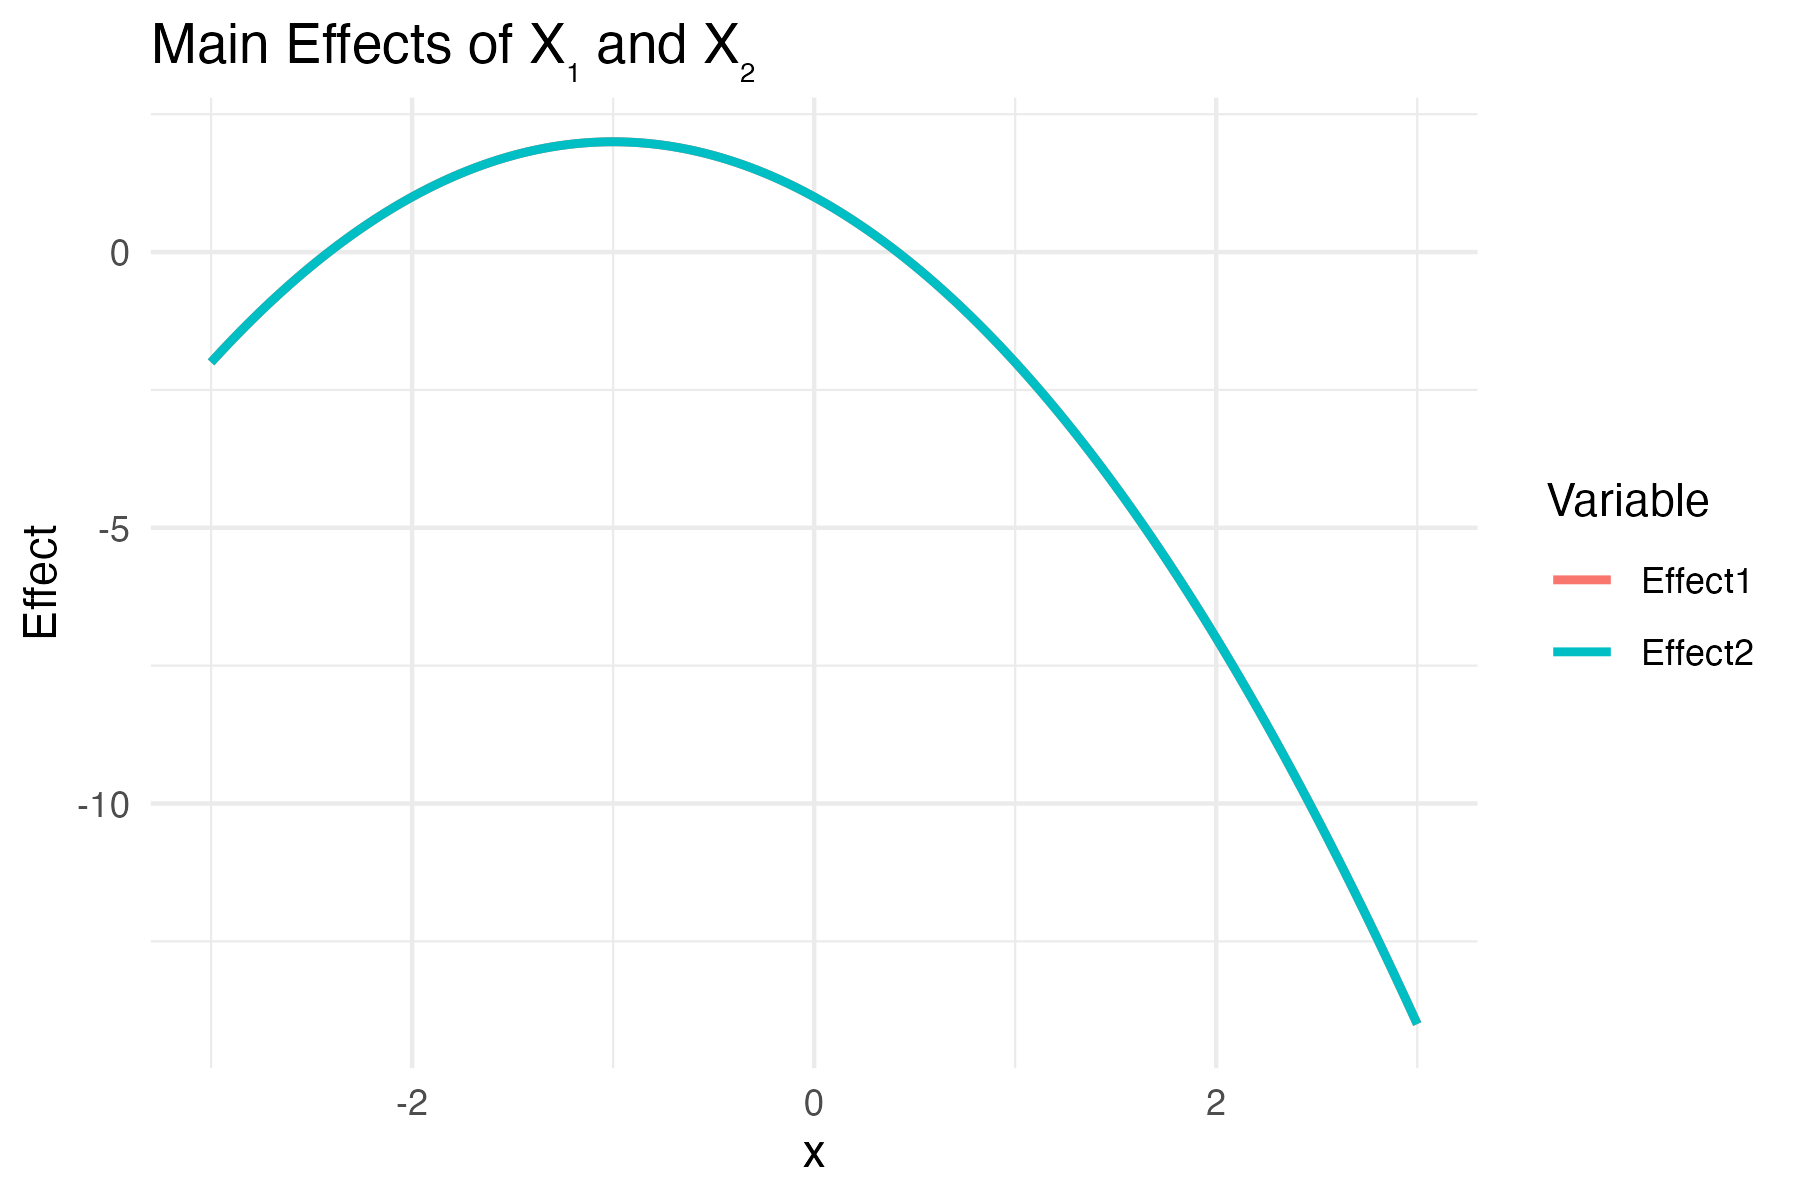
\includegraphics[width=\textwidth]{images/mixed_a1m20_a2m20_a11m10_a22m10_a12p00_rhop00_main.png}
    \end{minipage}
    \hfill
    \begin{minipage}[t]{0.49\textwidth}
        \centering
        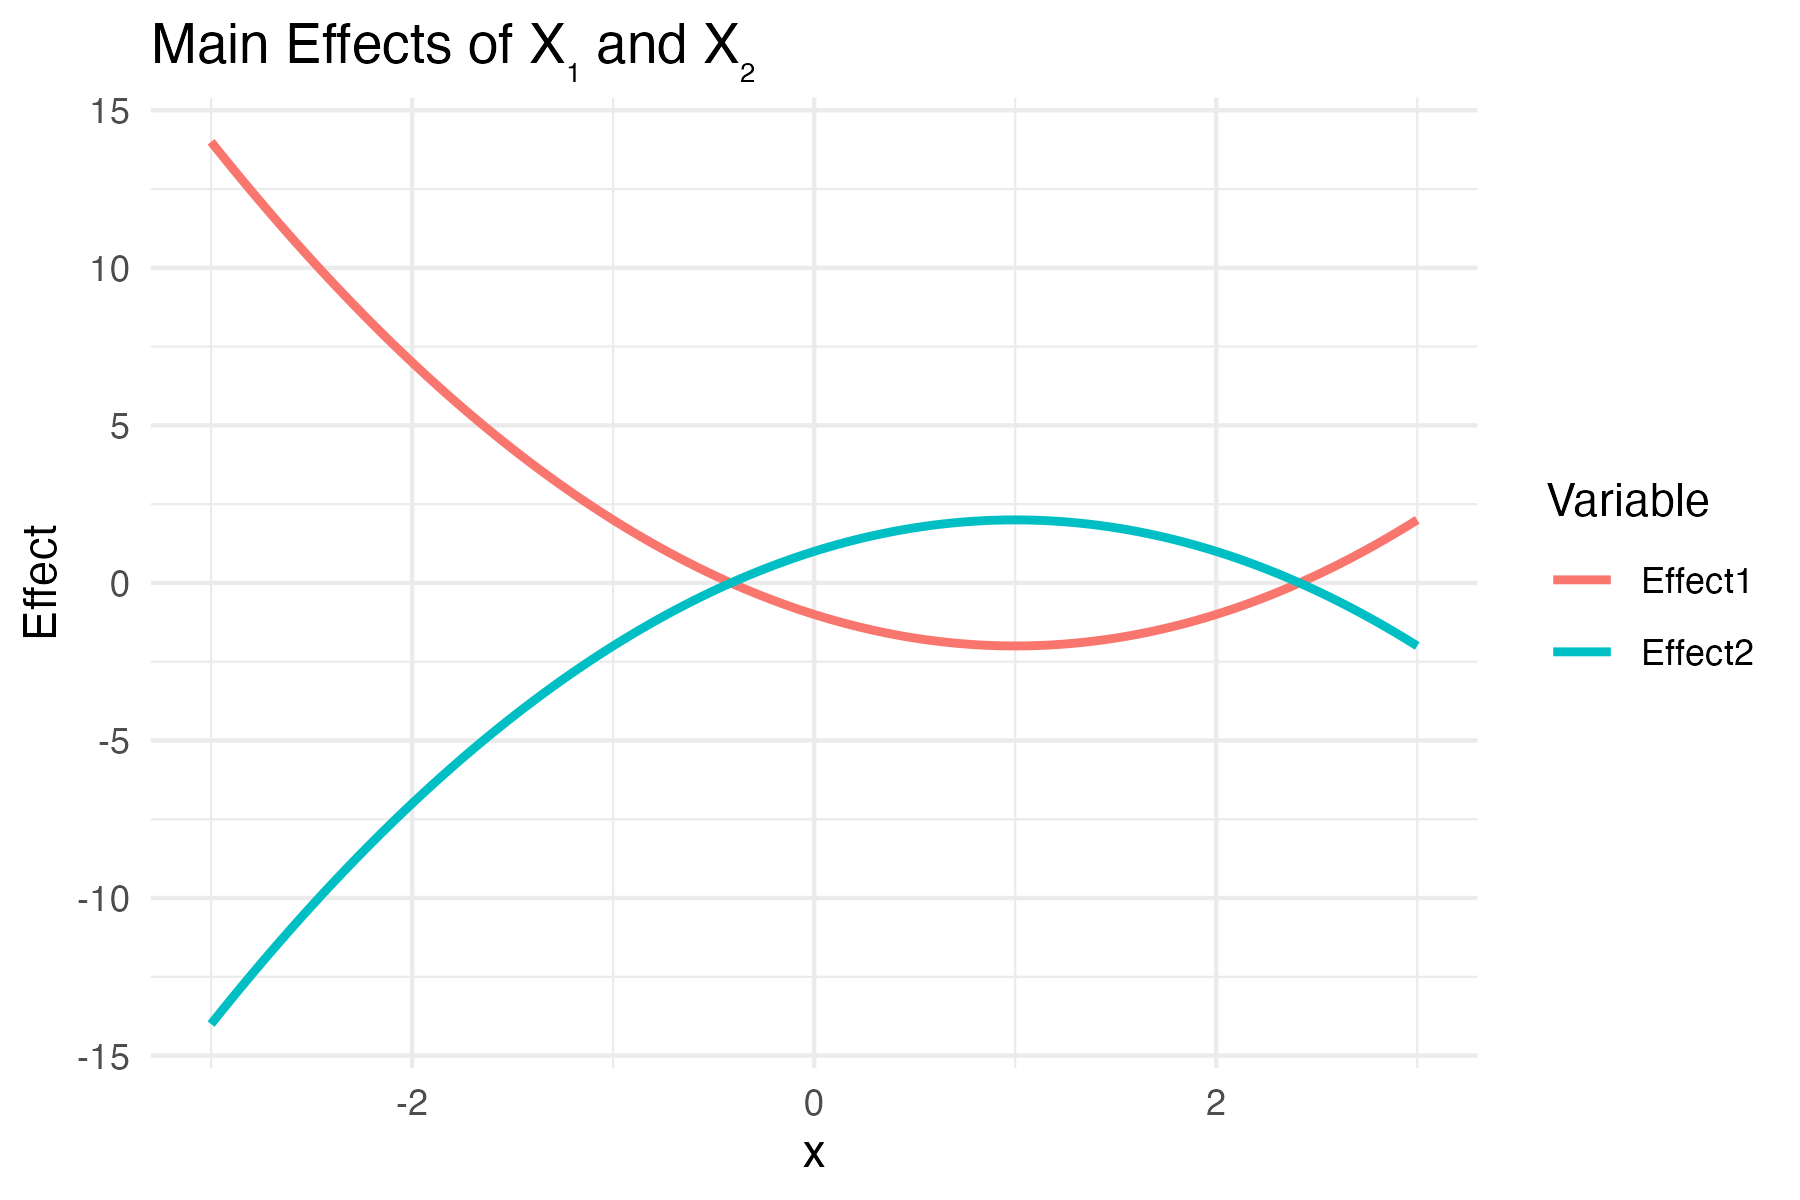
\includegraphics[width=\textwidth]{images/mixed_a1m20_a2p20_a11p10_a22m10_a12p00_rhop00_main.png}
    \end{minipage}
    \hfill
    \begin{minipage}[t]{0.49\textwidth}
        \centering
        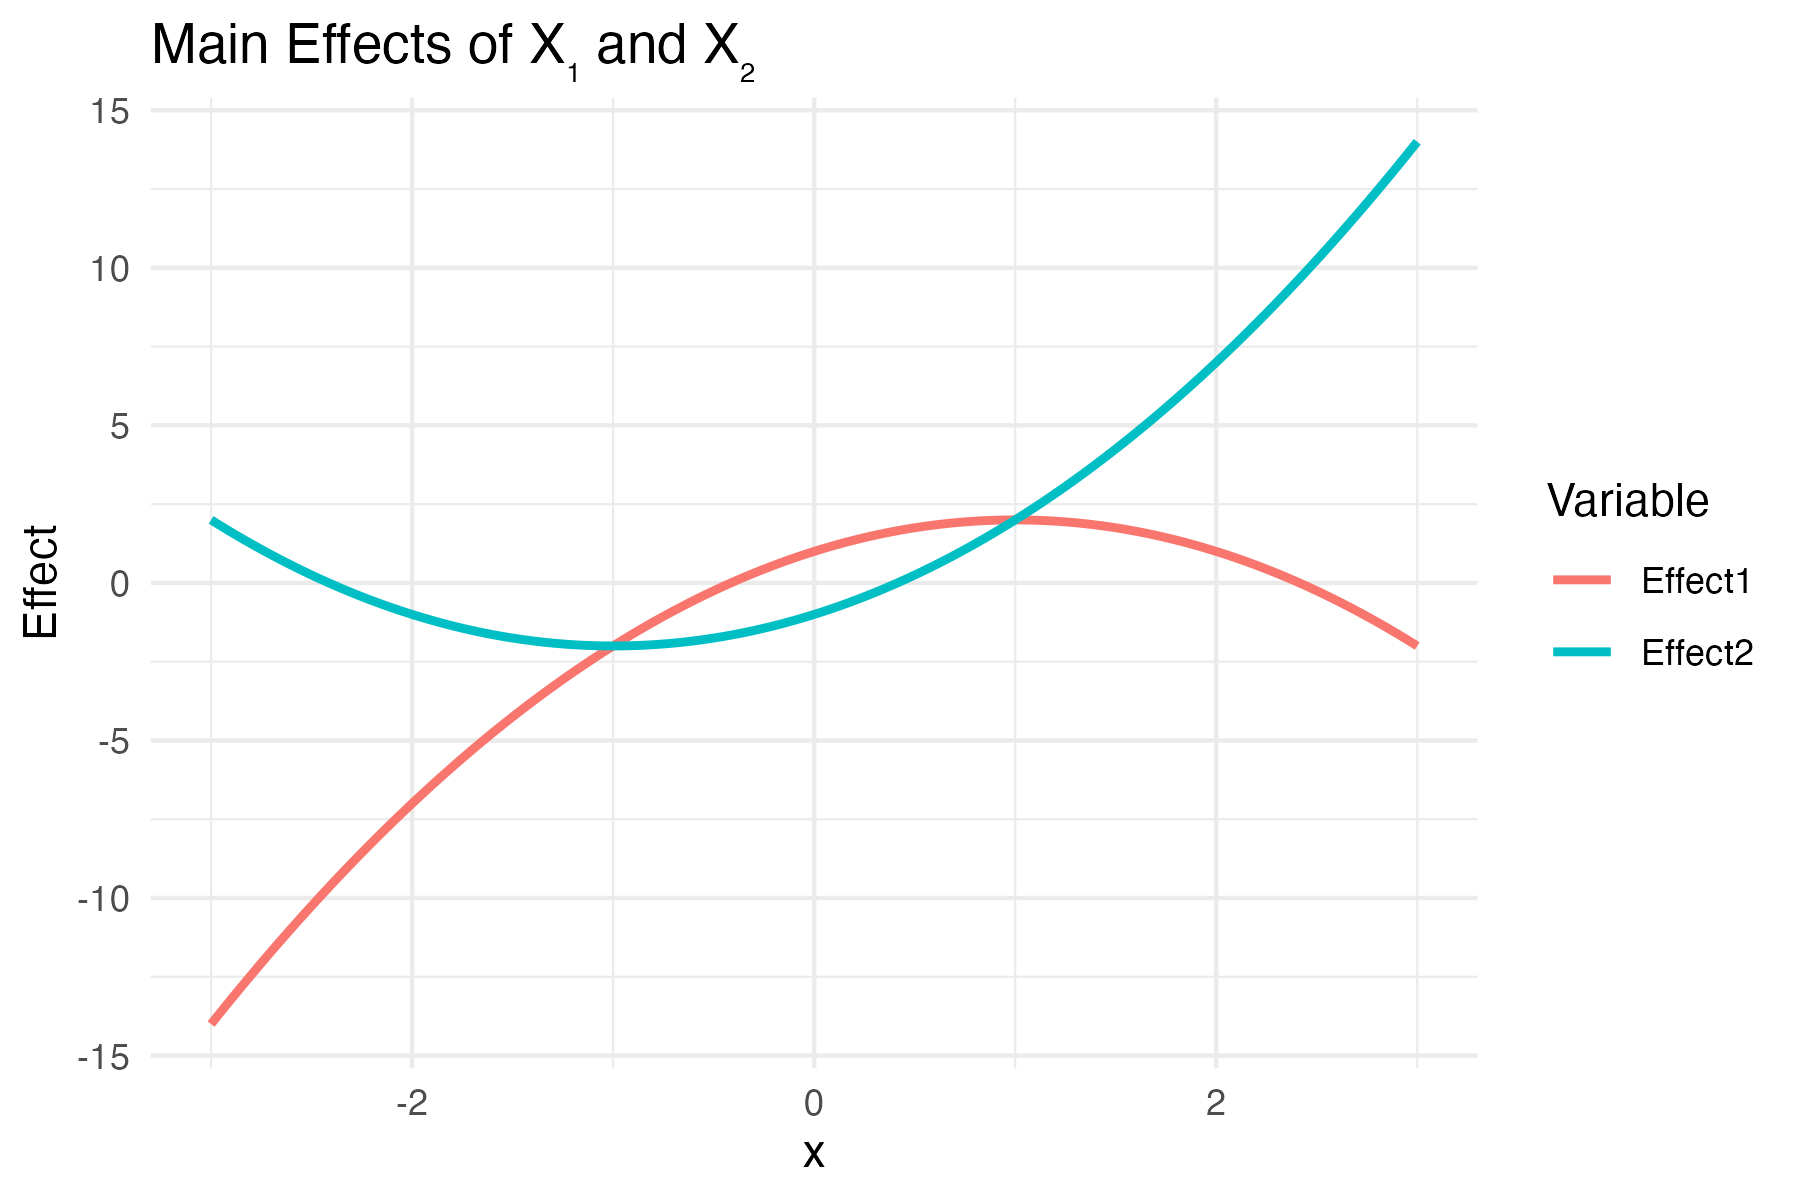
\includegraphics[width=\textwidth]{images/mixed_a1p20_a2p20_a11m10_a22p10_a12p00_rhop00_main.png}
    \end{minipage}
    \hfill
    \begin{minipage}[t]{0.49\textwidth}
        \centering
        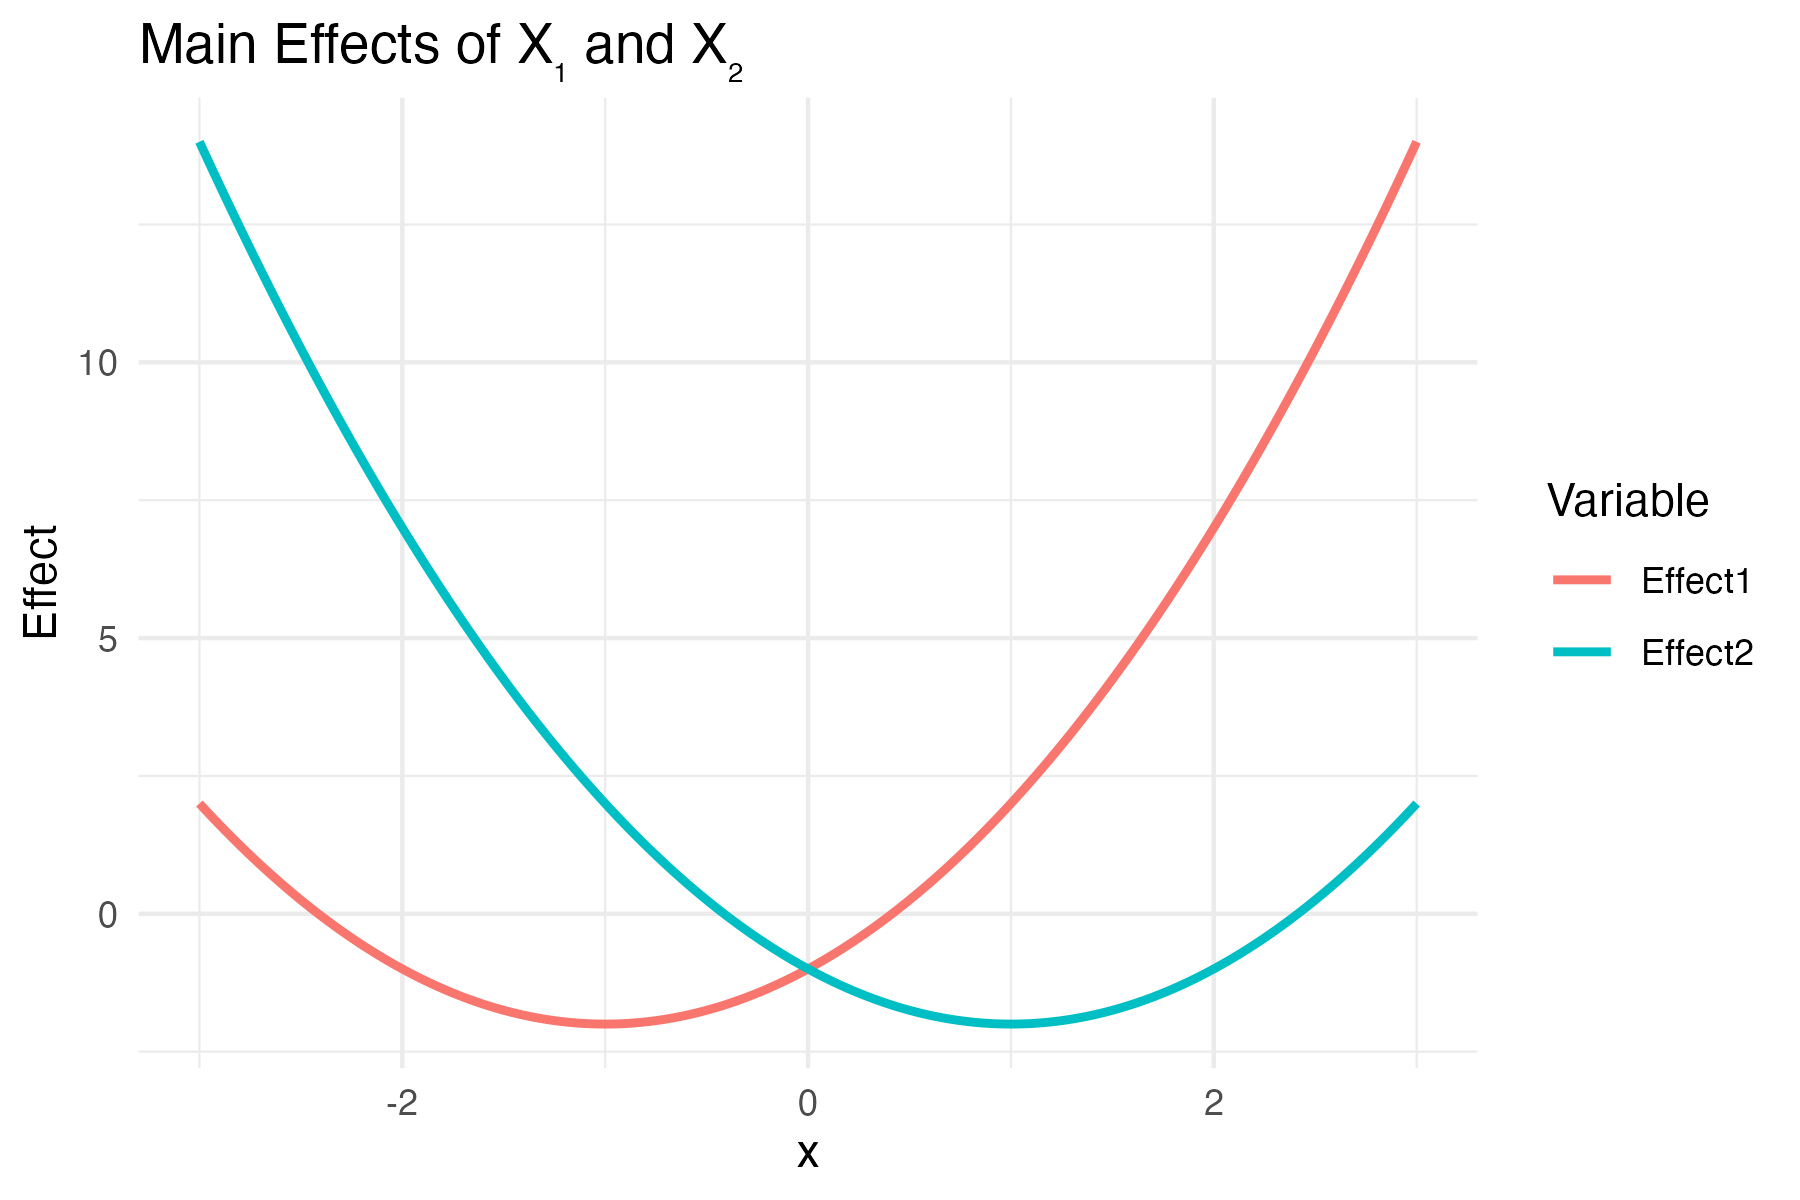
\includegraphics[width=\textwidth]{images/mixed_a1p20_a2m20_a11p10_a22p10_a12p00_rhop00_main.png}
    \end{minipage}
    \caption{Main effects and contour plot of different coefficients for mixed main effects.}
    \label{fig:mixed_rho_0}
\end{figure}
\begin{align*}
y_0 &= -2 \\[3pt]
y_1(x_1) &= -2x_1 - (x_1^2 - 1) \\[3pt]
y_2(x_2) &= -2x_2 - (x_2^2 - 1)
\end{align*}

\begin{align*}
y_1(x_1) &= -2x_1 + (x_1^2 - 1) \\[3pt]
y_2(x_2) &= 2x_2 - (x_2^2 - 1)
\end{align*}

\begin{align*}
y_1(x_1) &= 2x_1 - (x_1^2 - 1) \\[3pt]
y_2(x_2) &= 2x_2 + (x_2^2 - 1)
\end{align*}


\subsubsection*{Scenario: All}
Finally full example, including all main and interaction effects: $$g_5(x_1, x_2) = a_1 x_1 + a_2 x_2 + a_{11} x_1^2 + a_{22} x_2^2 + a_{12} x_1 x_2,$$ where we can very the coefficients as well as $\rho$.\par
We recognize the patterns from previous examples which had less parameters to vary. If the parabolas are facing upwards or downwards is determined by the sign of the quadratic coefficients; if they are facing in the same direction is determined by between variable sign-difference of the quadratic coefficients. Under presence of an interaction term, how strongly the variables correlate with each other also affects the direction in which the main effects are facing. How stretched or compressed the parabolas are is determined by the linear coefficients. The interaction term is determined by the sign and magnitude of $\rho$ as well as the sign and magnitude of the interaction coefficient $a_{12}$.\par
\begin{figure}[htpb]
    \centering
    \begin{minipage}[t]{0.49\textwidth}
        \centering
        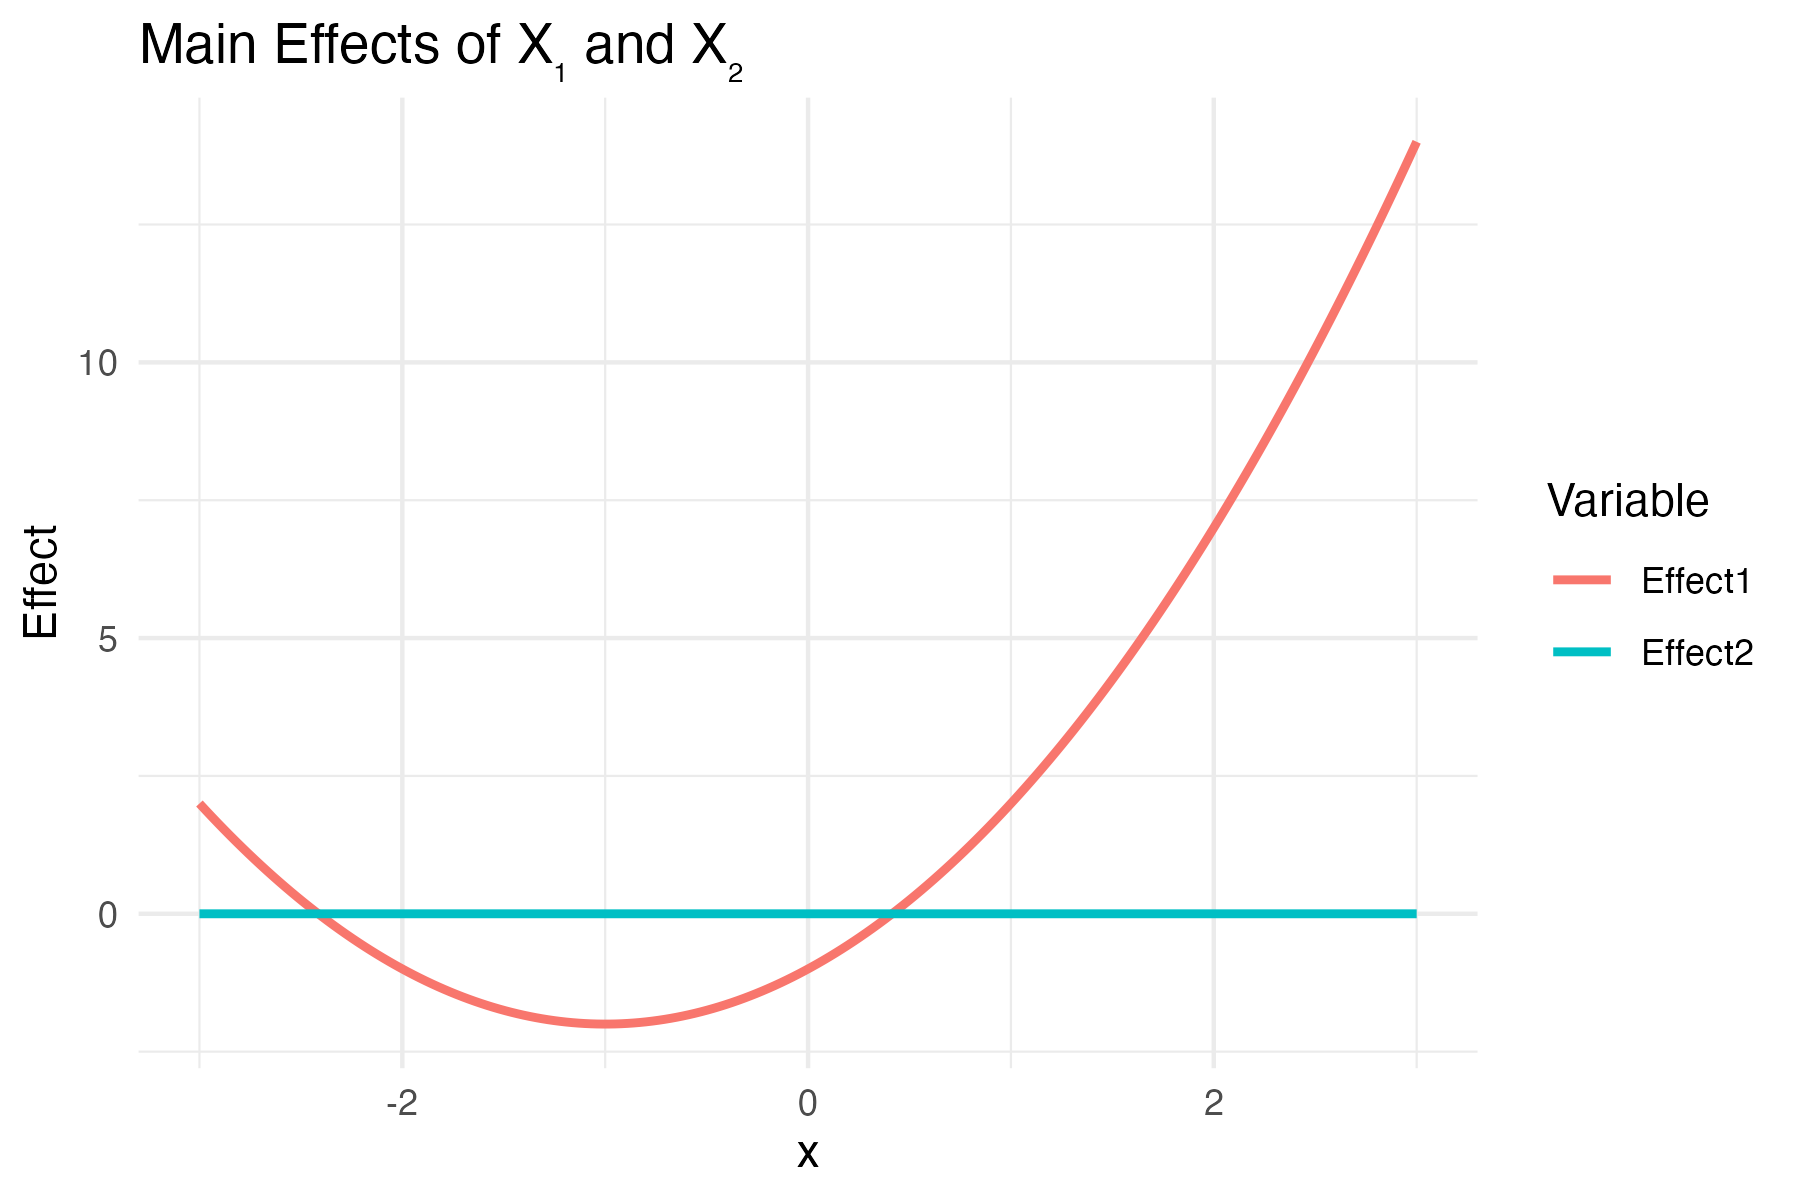
\includegraphics[width=\textwidth]{images/full_a1p20_a2p00_a11p10_a22p00_a12p05_rhop00_main.png}
    \end{minipage}%
    \hfill
    \begin{minipage}[t]{0.49\textwidth}
        \centering
        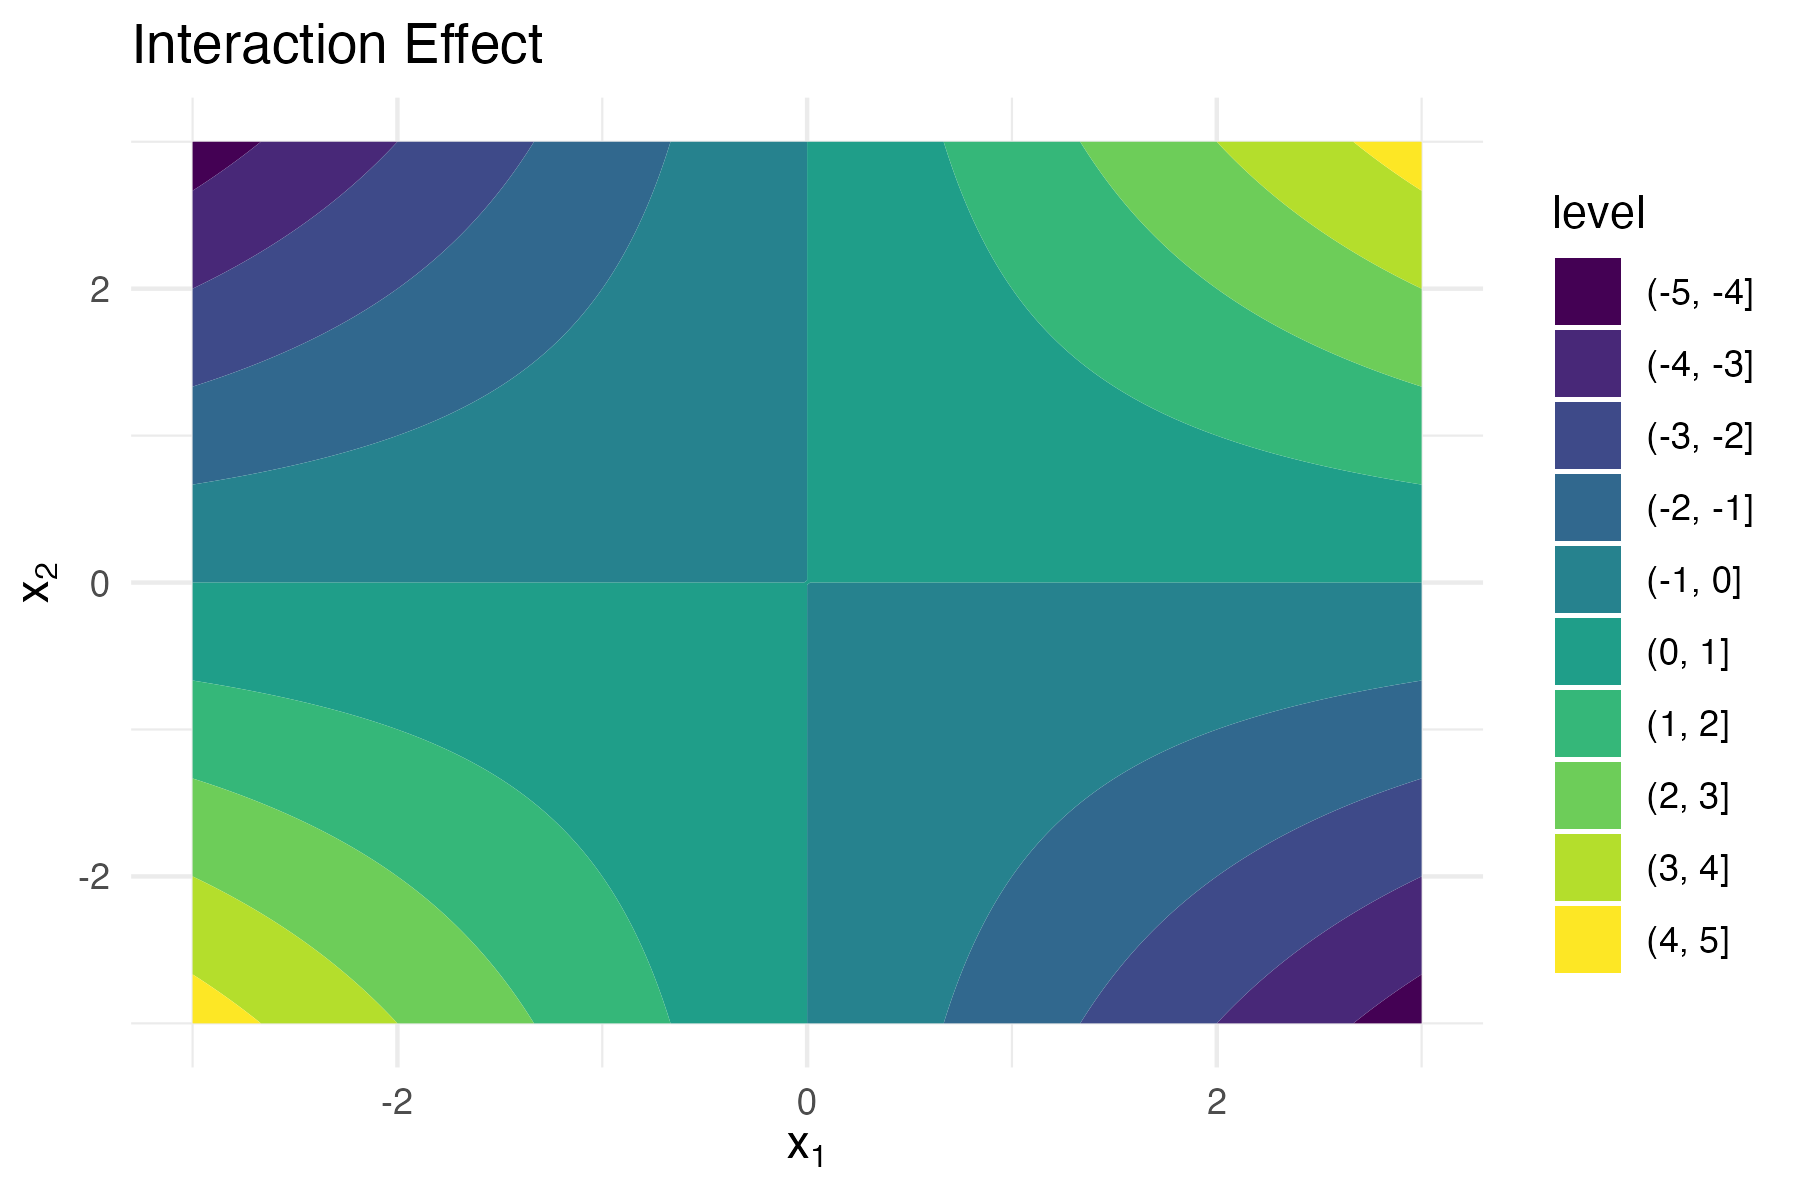
\includegraphics[width=\textwidth]{images/full_a1p20_a2p00_a11p10_a22p00_a12p05_rhop00_interaction.png}
        \caption{Main effects and contour plot of interaction effects for $g(x) = x_1 + 2 x_2 + x_1 x_2$ with independent inputs, $\rho = 0$.}
        \label{fig:full_rho_0}
    \end{minipage}
\end{figure}


\begin{figure}[htpb]
    \centering
    \begin{minipage}[t]{0.49\textwidth}
        \centering
        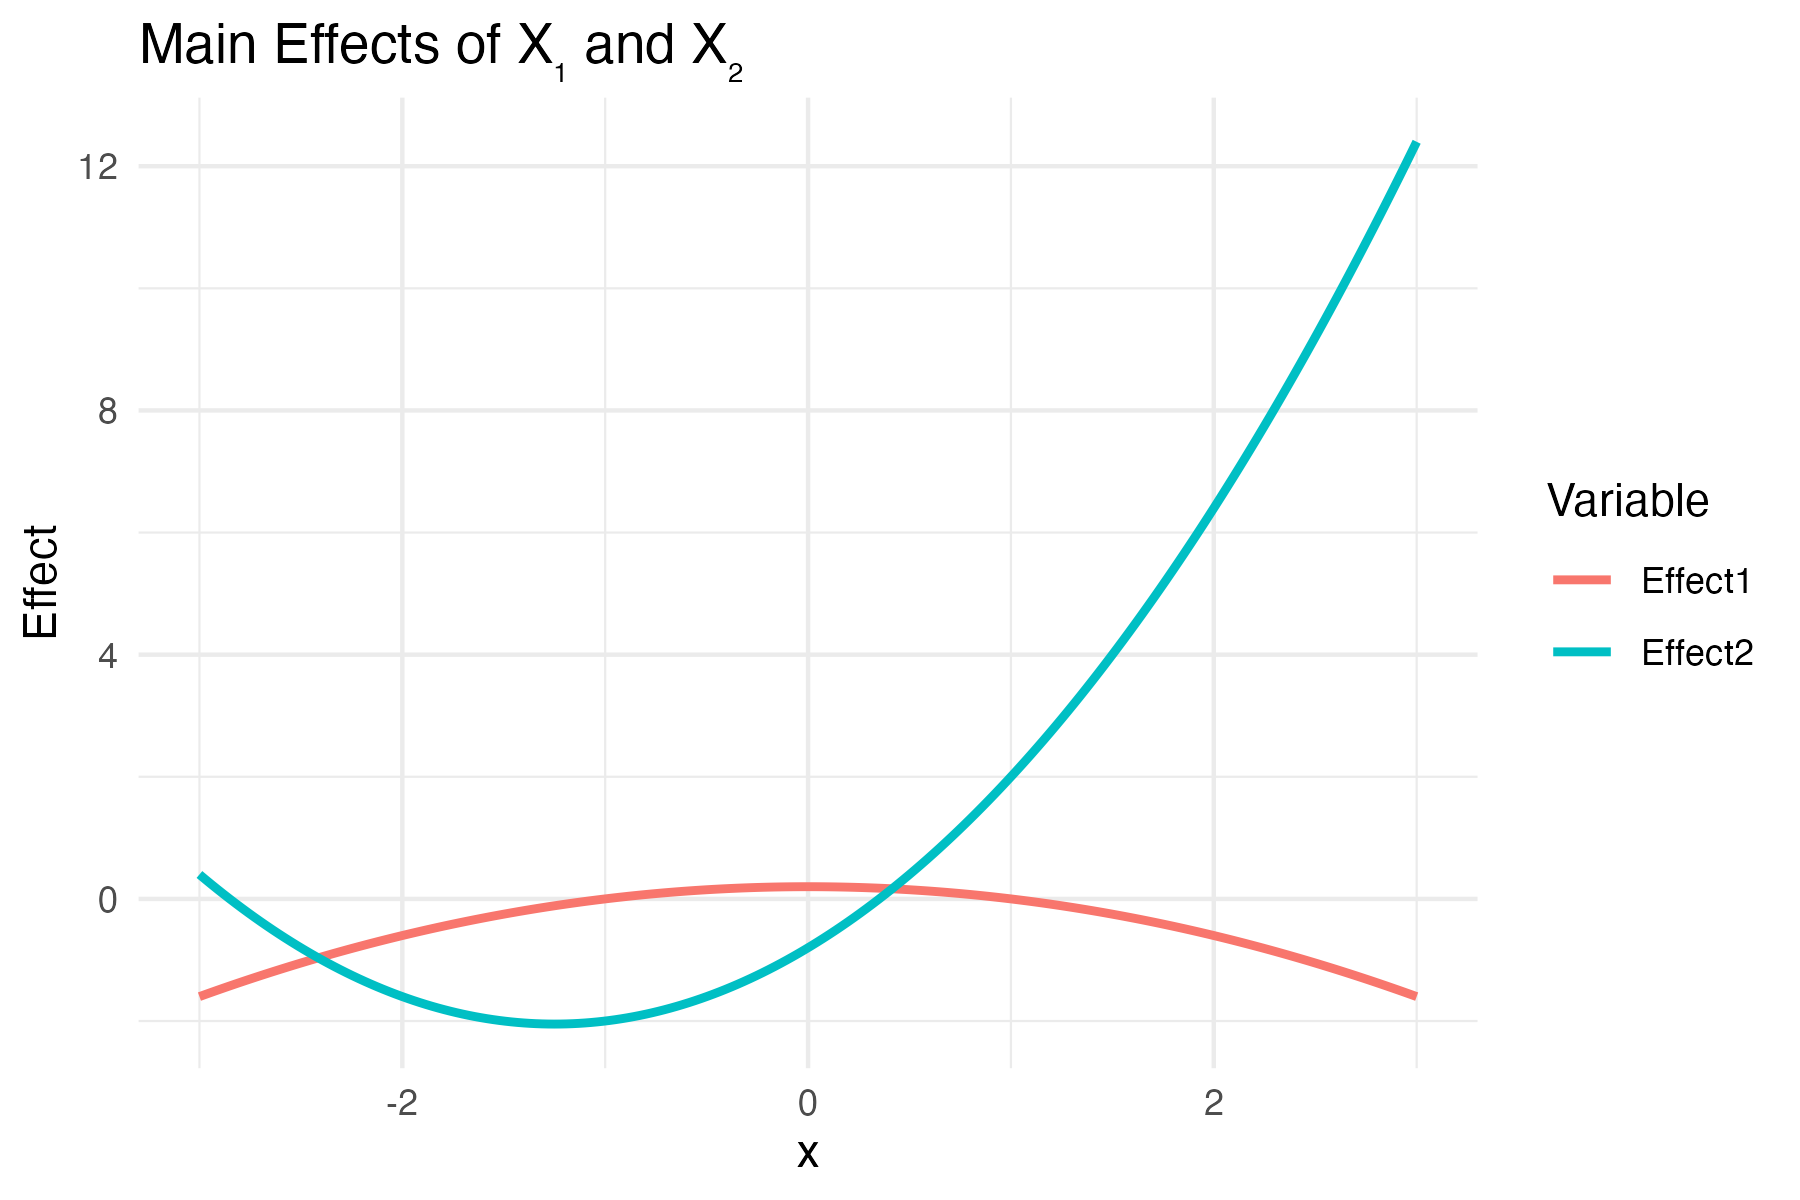
\includegraphics[width=\textwidth]{images/full_a1p00_a2p20_a11p00_a22p10_a12m05_rhop05_main.png}
    \end{minipage}%
    \hfill
    \begin{minipage}[t]{0.49\textwidth}
        \centering
        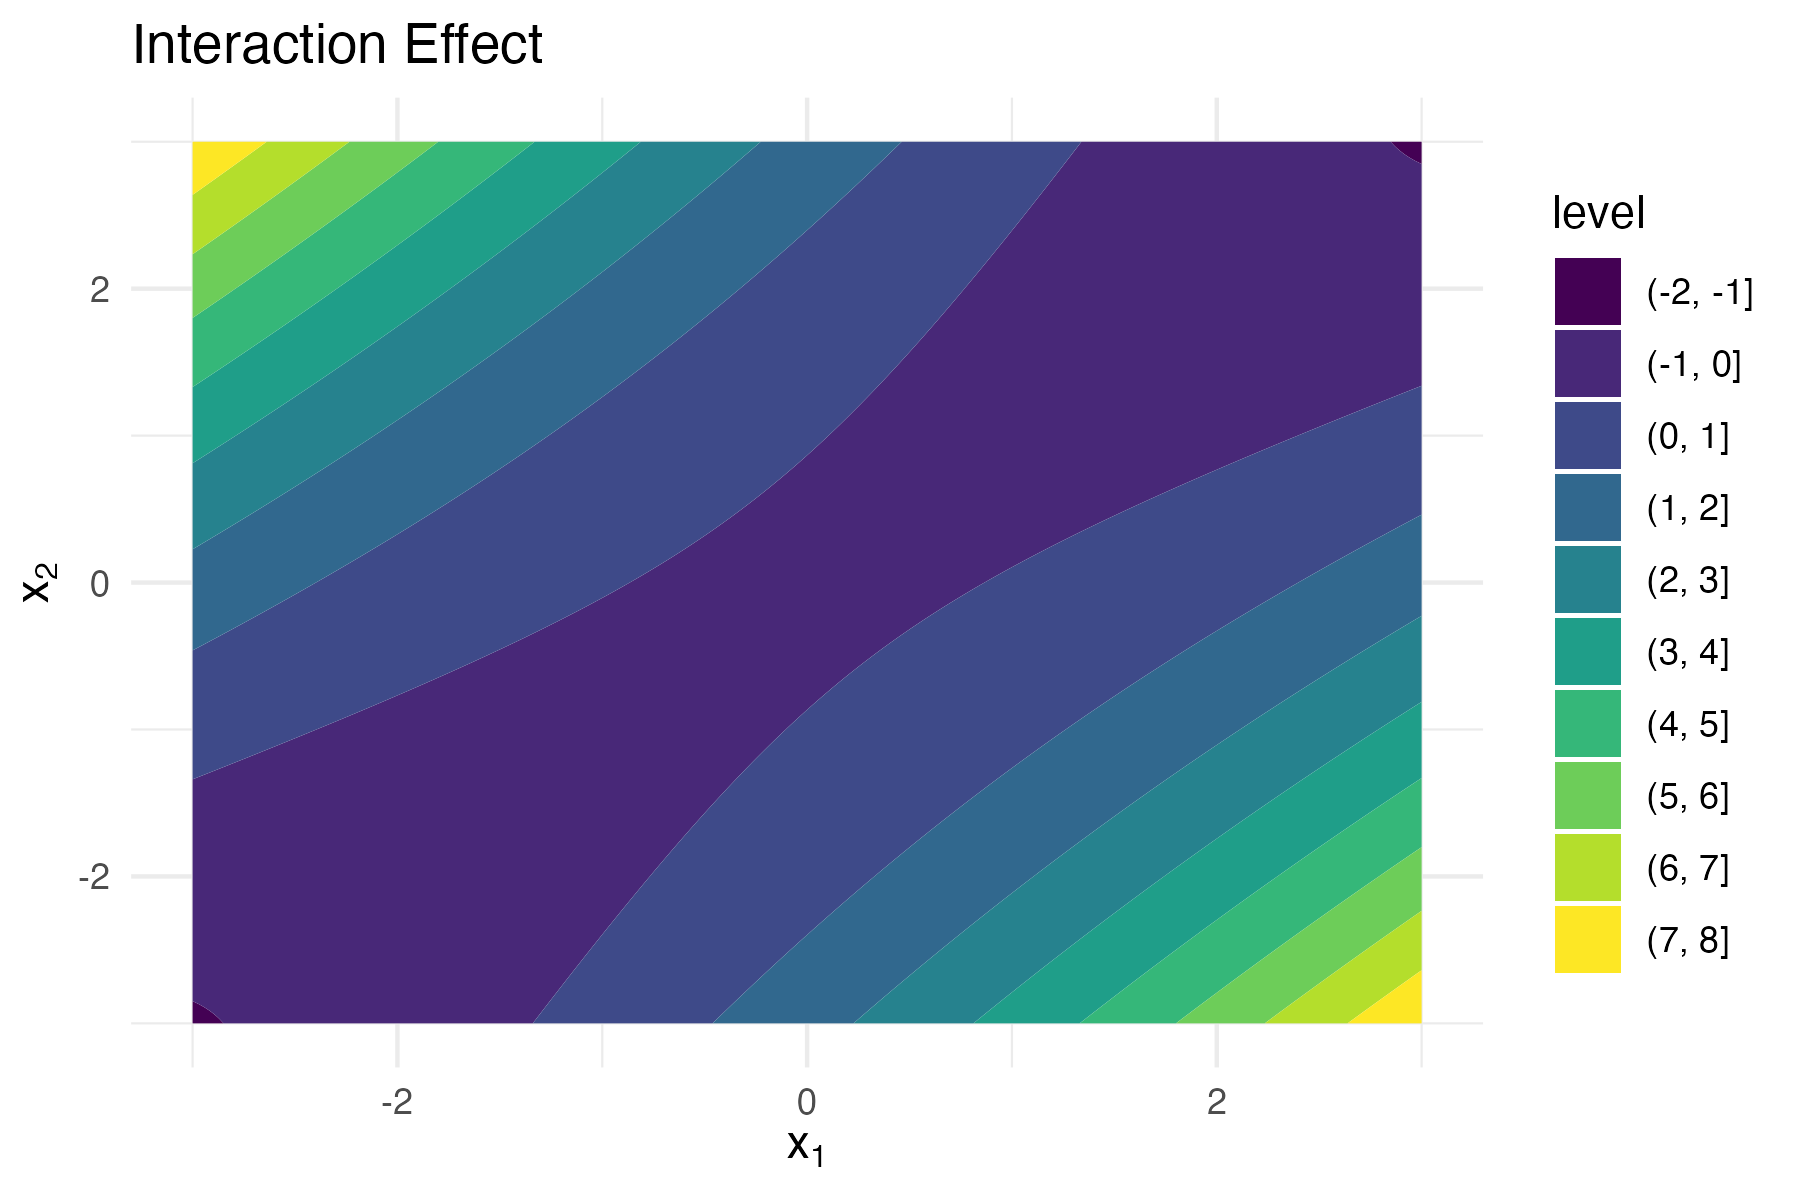
\includegraphics[width=\textwidth]{images/full_a1p00_a2p20_a11p00_a22p10_a12m05_rhop05_interaction.png}
        \caption{Main effects and contour plot of interaction effects for $g(x) = x_1 + 2 x_2 + x_1 x_2$ with dependent inputs, $\rho = -0.5$.}
        \label{fig:full_rho_neg0.5}
    \end{minipage}
\end{figure}


\begin{figure}[htpb]
    \centering
    \begin{minipage}[t]{0.49\textwidth}
        \centering
        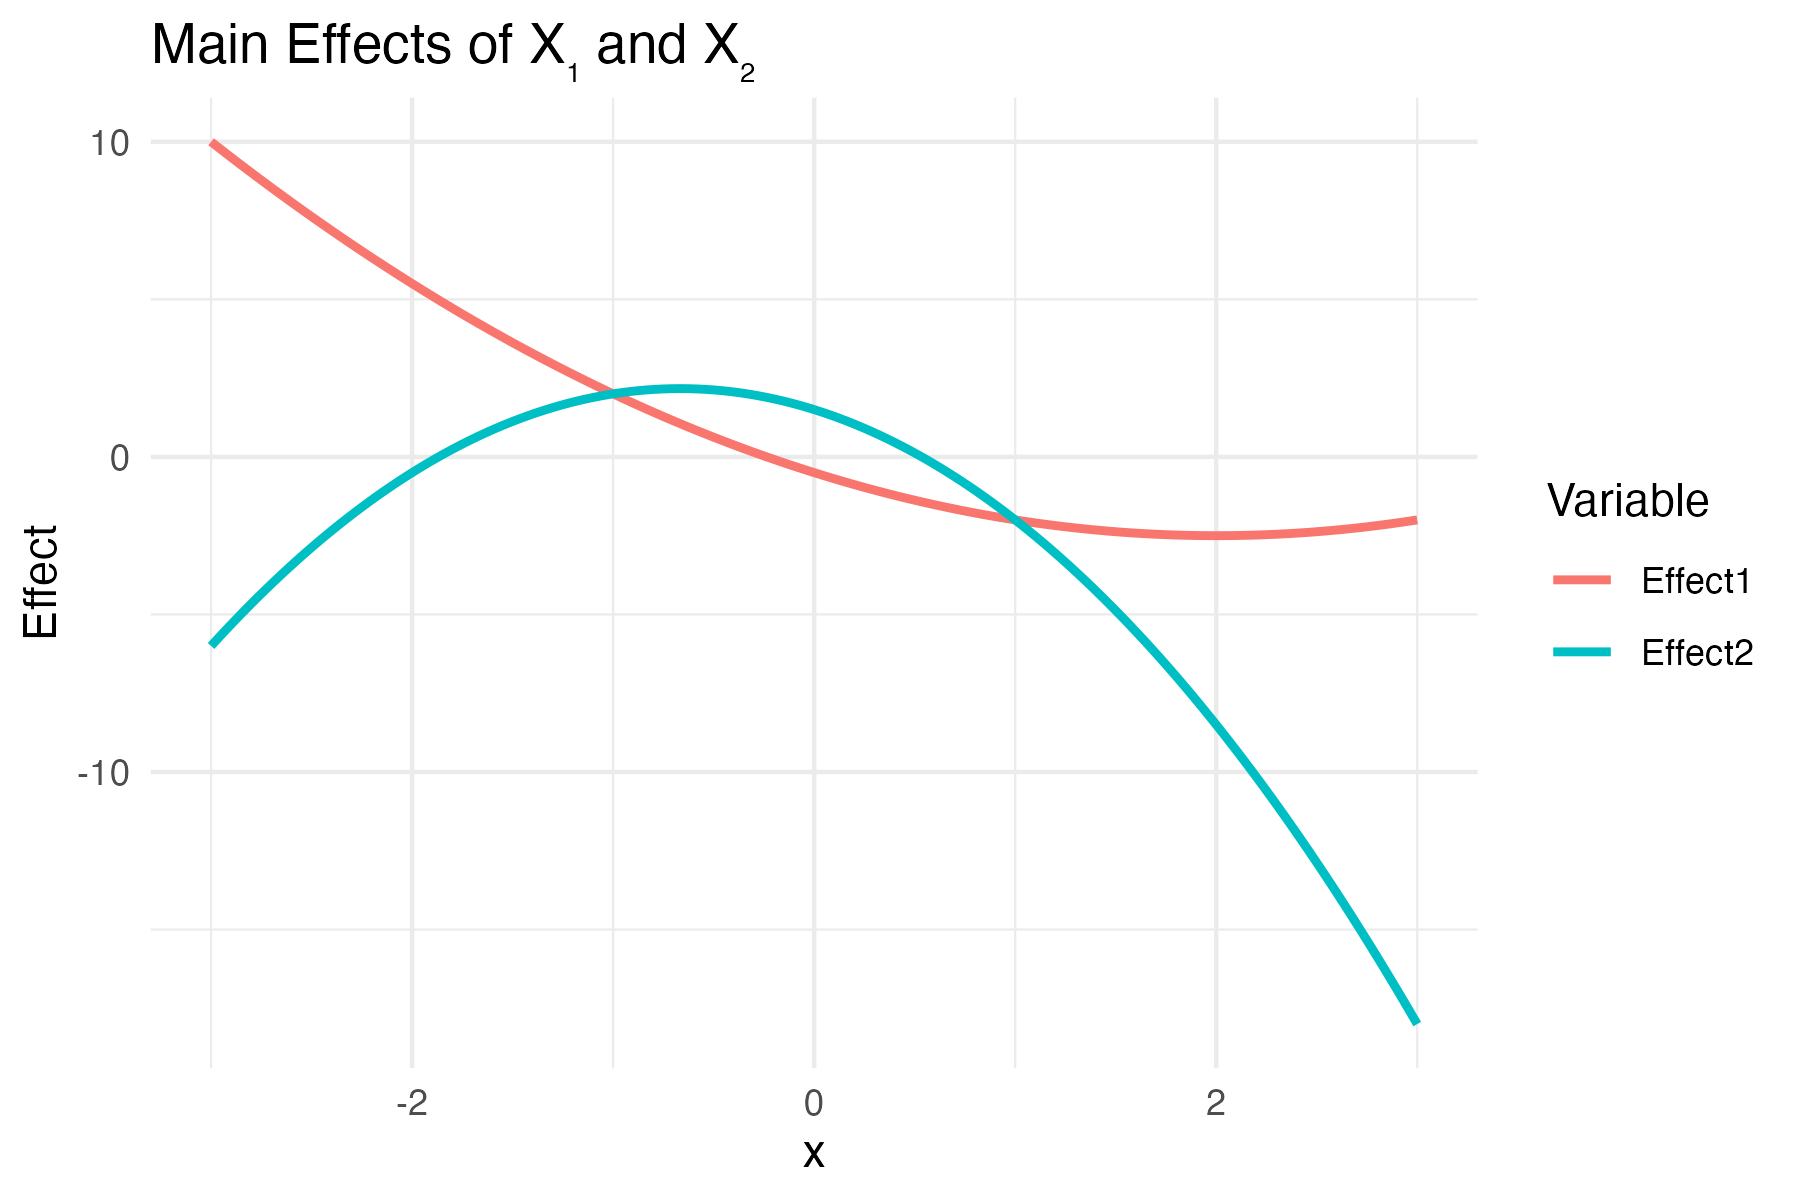
\includegraphics[width=\textwidth]{images/full_a1m20_a2m20_a11p10_a22m10_a12p10_rhom10_main.png}
    \end{minipage}%
    \hfill
    \begin{minipage}[t]{0.49\textwidth}
        \centering
        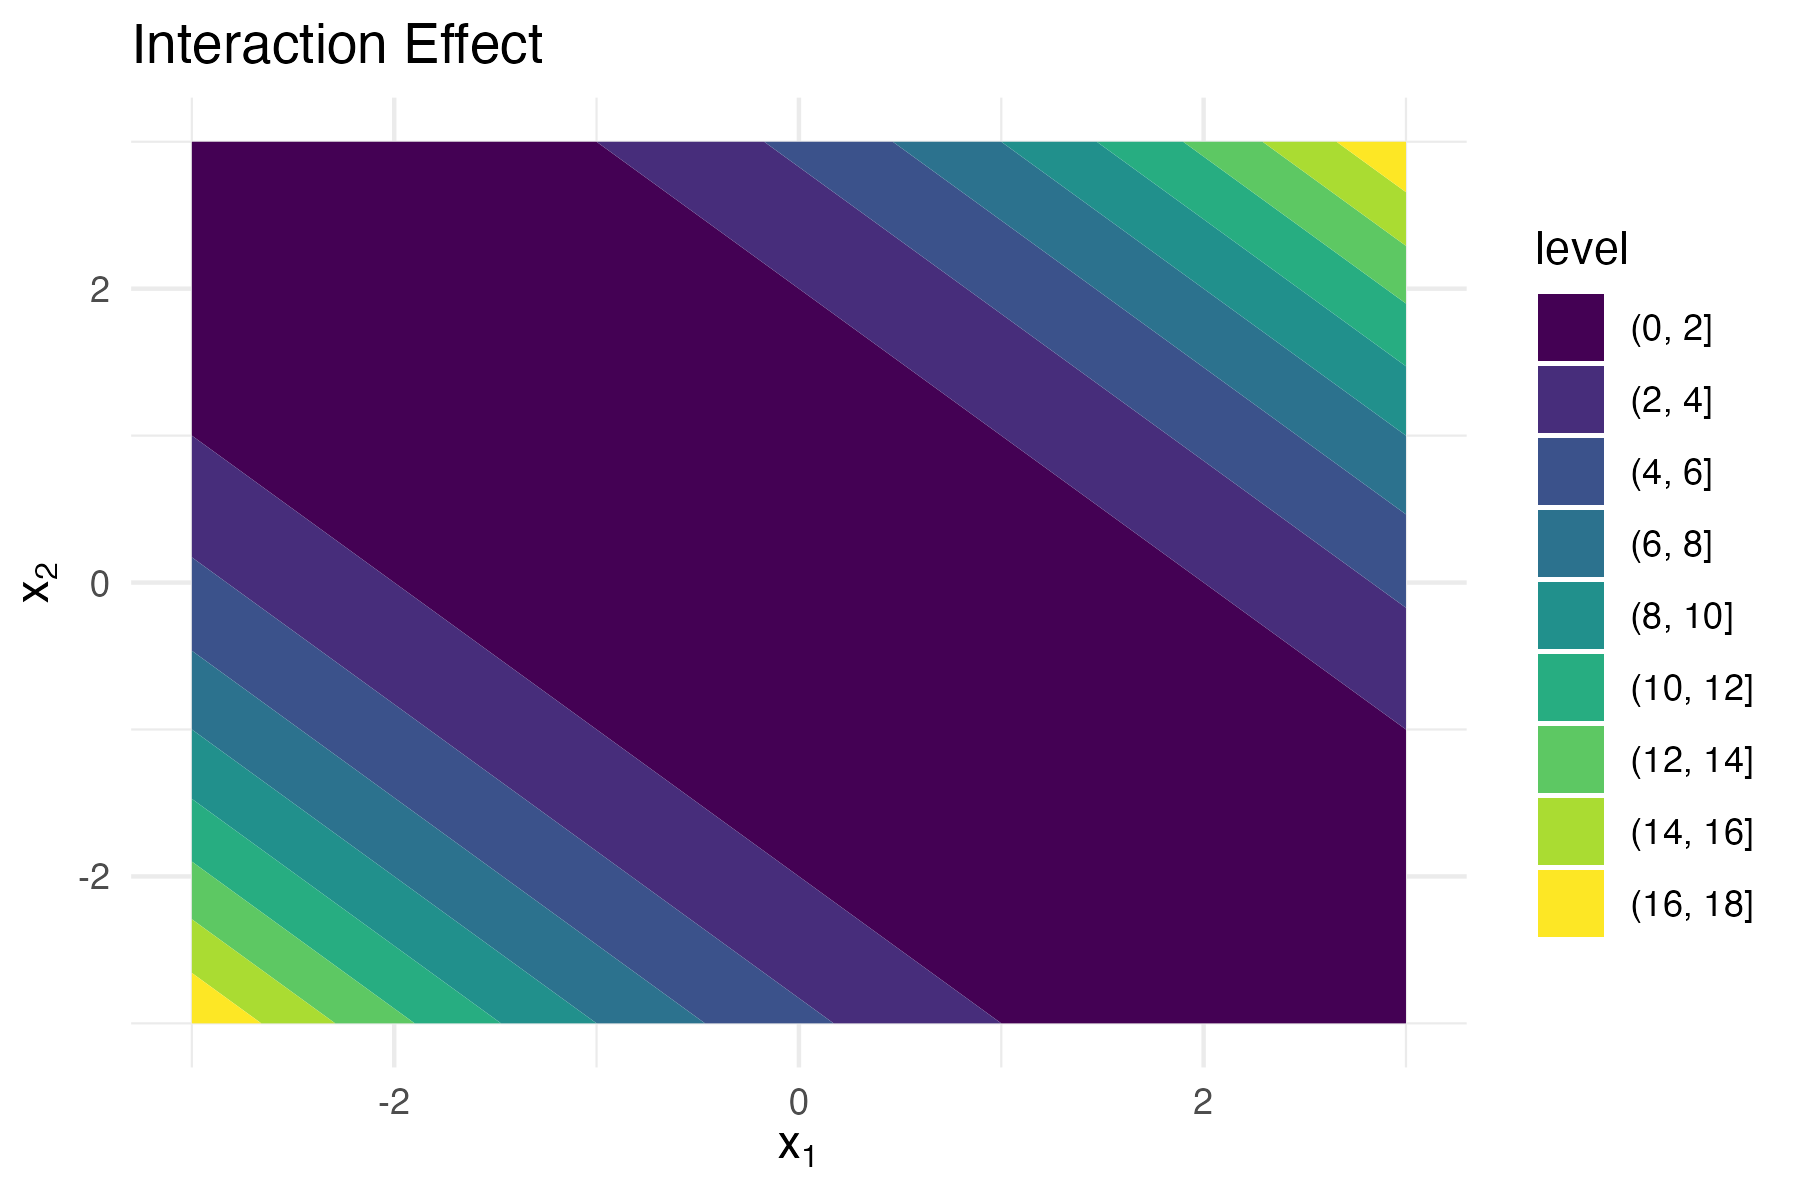
\includegraphics[width=\textwidth]{images/full_a1m20_a2m20_a11p10_a22m10_a12p10_rhom10_interaction.png}
        \caption{Main effects and contour plot of interaction effects for $g(x) = x_1 + 2 x_2 + x_1 x_2$ with dependent inputs, $\rho = -0.5$.}
        \label{fig:full_rho_neg1}
    \end{minipage}
\end{figure}


\begin{figure}[htpb]
    \centering
    \begin{minipage}[t]{0.49\textwidth}
        \centering
        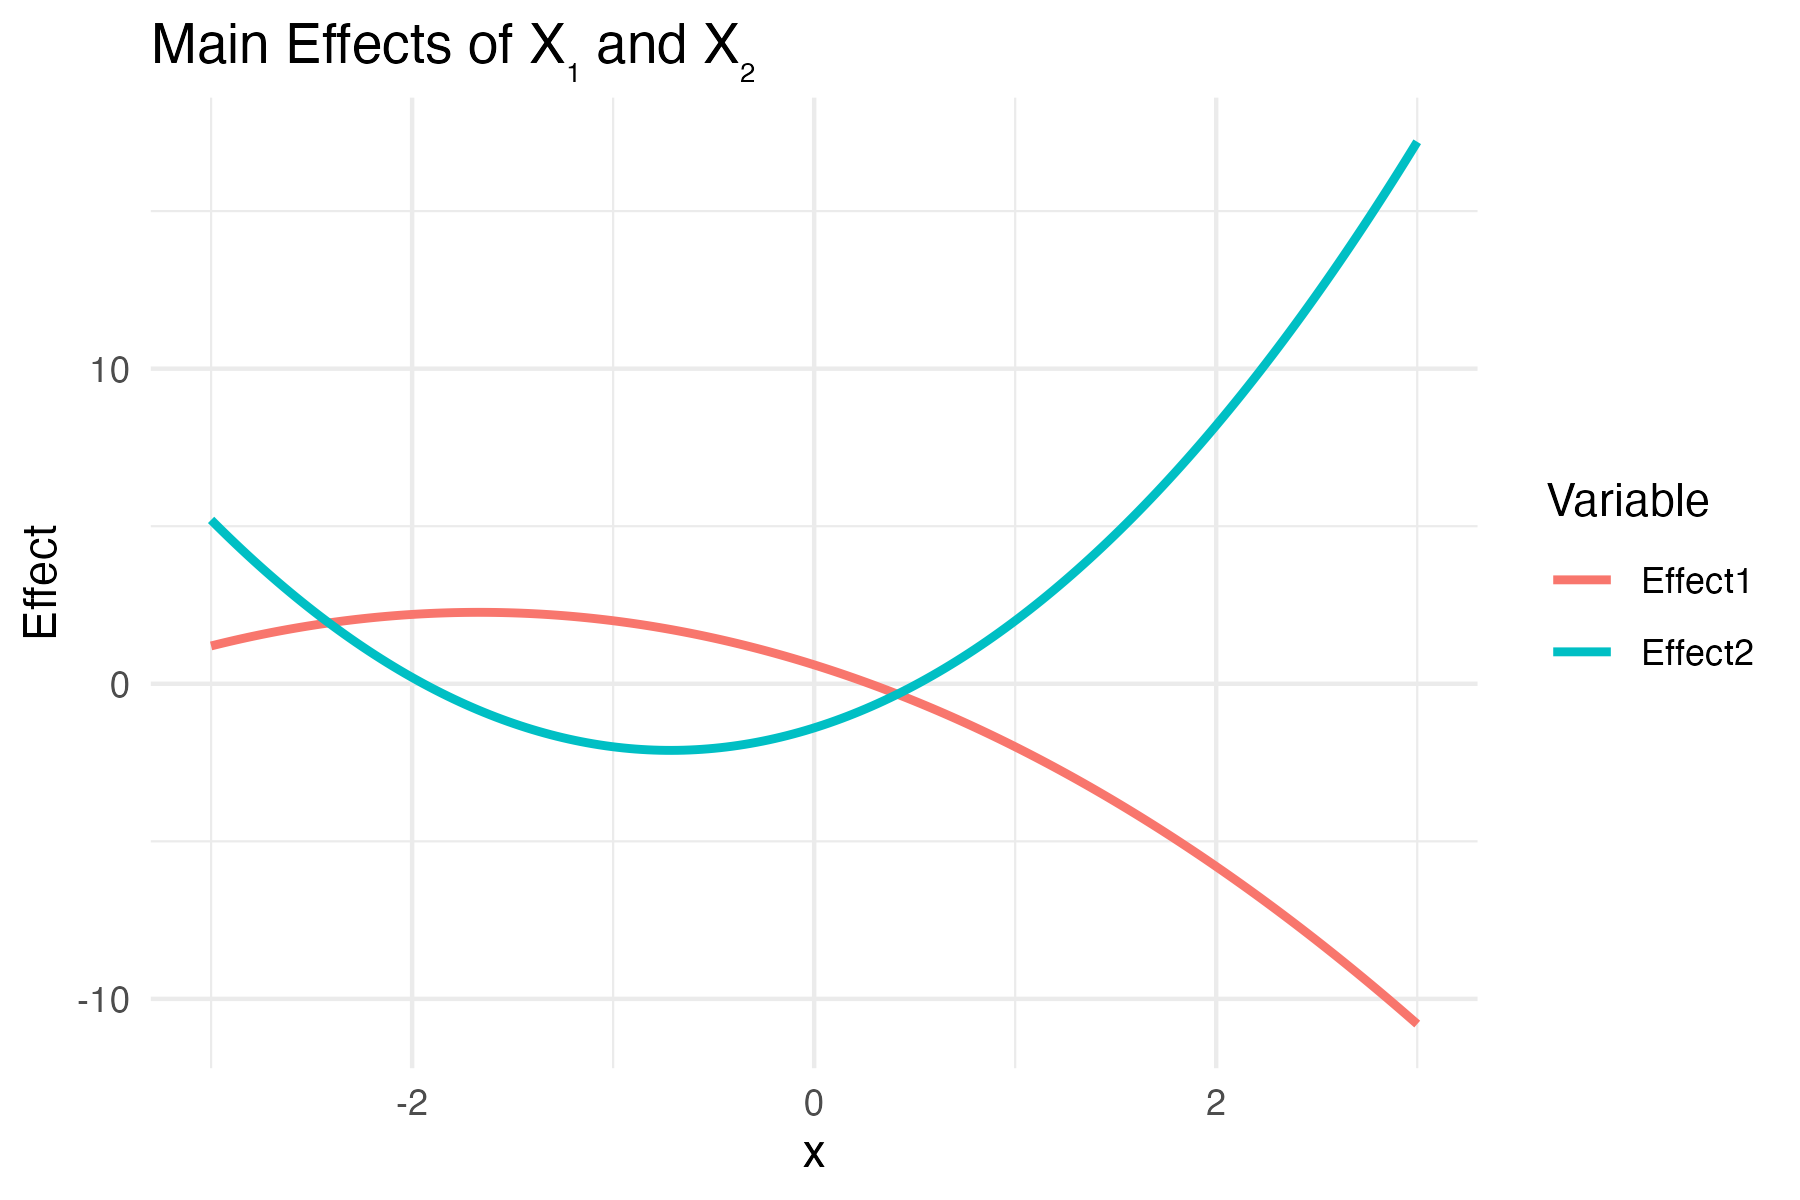
\includegraphics[width=\textwidth]{images/full_a1m20_a2p20_a11m10_a22p10_a12m10_rhom05_main.png}
    \end{minipage}%
    \hfill
    \begin{minipage}[t]{0.49\textwidth}
        \centering
        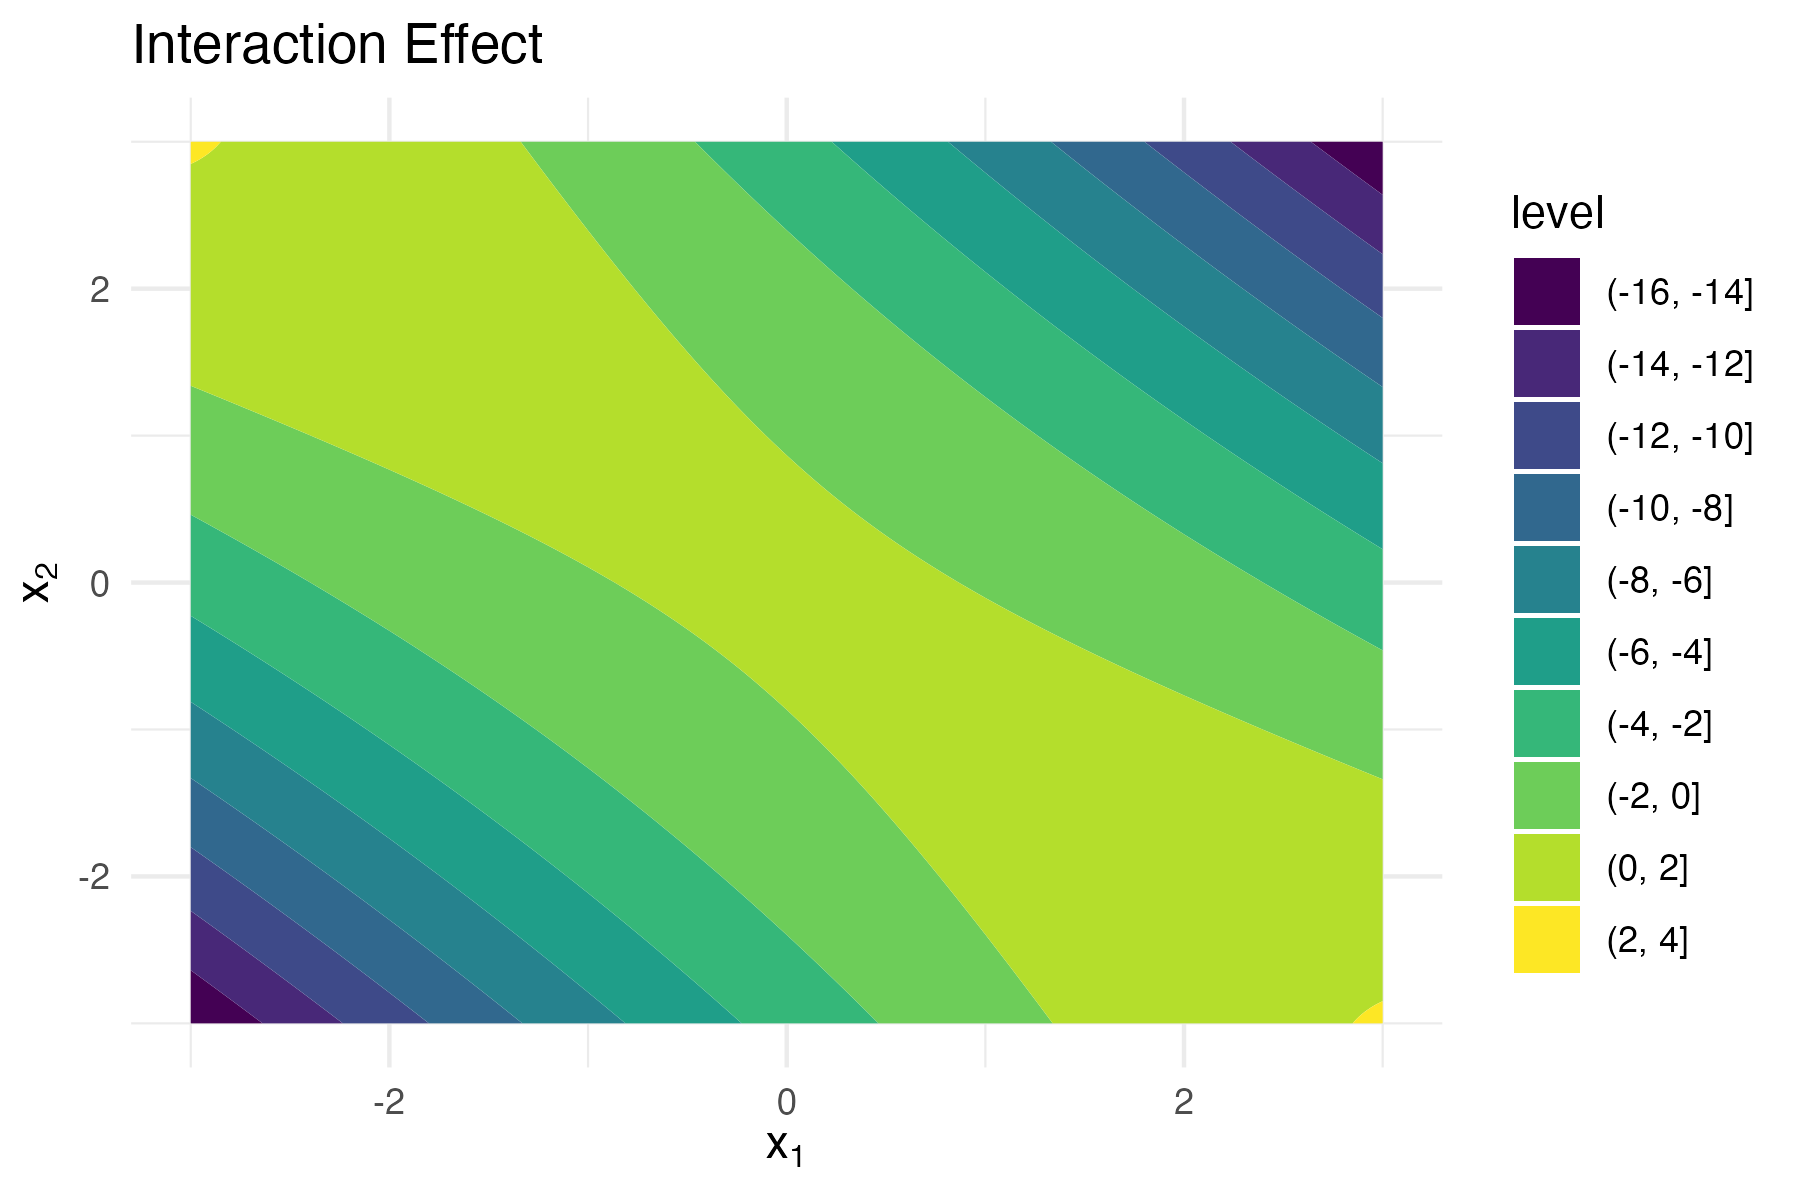
\includegraphics[width=\textwidth]{images/full_a1m20_a2p20_a11m10_a22p10_a12m10_rhom05_interaction.png}
        \caption{Main effects and contour plot of interaction effects for $g(x) = x_1 + 2 x_2 + x_1 x_2$ with dependent inputs, $\rho = 0.5$.}
        \label{fig:full_rho_pos0.5}
    \end{minipage}
\end{figure}